\section{Preliminary Results and Findings}
\label{sec:preliminary_results}

This section presents the results obtained from training a subset of the algorithms discussed in section \ref{subsec:algorithm_selection}. The selected algorithms include five DQN-based methods — DQN, Double DQN, Prioritized Experience Replay, Dueling DQN, and C51 — as well as three policy-based methods: REINFORCE, PPO, and SAC. Soft Actor Critic was preferred to DDPG and TD3 because it can simply be seen as a variation that works with a stochastic policy, but is more easily adapted to a discrete action space.

We first describe necessary modifications to the experiment setup, followed by a detailed analysis of each algorithm's performance and emissions. The results are then compared across different algorithm families.

\subsection{Experiment Setup Adjustments}
\label{subsec:exp_setup_adjustments}
During initial training attempts, some adjustments were required to ensure reliable performance and energy tracking. One key reason for this was that employing CodeCarbon as a (next-)real-time emissions tracking tool significantly slowed down training (by a factor of 20 or more). As a result, we opted to record only total emissions at the end of training rather than tracking them continously. This adjustment allowed us to obtain meaningful comparisons without excessively increasing training time.

In addition to this, on Windows, CodeCarbon's CPU energy tracking relies on the Intel Power Gadget, which has been deprecated for several years. Furthermore, it does not support Intel Performance Counter Monitor (Intel PCM), the official successor to the Power Gadget. In such cases, CodeCarbon switches to a fallback mode, directly quoting from their documentation:
\begin{quoting}
	\begin{itemize}
		\item It will first detect which CPU hardware is currently in use, and then map it to a data source listing 2000+ Intel and AMD CPUs and their corresponding thermal design powers (TDPs).
		
		\item If the CPU is not found in the data source, a global constant will be applied. CodeCarbon assumes that 50\% of the TDP will be the average power consumption to make this approximation.
		
		\item We could not find any good resource showing statistical relationships between TDP and average power, so we empirically tested that 50\% is a decent approximation.
	\end{itemize}
\end{quoting}

This approach should provide reasonable estimates for our project, since most of the workload is on the GPU, while the rest is mostly constant across the algorithms (like the environment simulations). This being said, one instance where this limitation may have had an impact is in tracking the Proximal Policy Optimization (PPO) algorithm, that employs a relatively small neural network but requires more CPU and RAM processing, the latter also explicitly stated to not be tracked satisfactorily.

Moreover, wandb collect systems data, but it also, while collecting kwh for the gpu, does not for cpu and ram, so we have to make do with what we have

Additionally, Weights \& Biases collects system data during training, and while it tracks GPU energy consumption in kWh, it also does not do the same for CPU and RAM. As a result, while we can obtain excellent emissions estimates for the GPU, CPU and RAM energy tracking remains imprecise due to the aforementioned limitations. Consequently, energy consumption analyses must be interpreted with an understanding of these constraints.

\subsection{DQN-Based Algorithms}
We present the results for the five different DQN-based algorithms. Each algorithm is analyzed individually before an overall comparison.

\subsubsection{Deep Q-Network (DQN Baseline)}
\label{subsubsec:dqn_baseline}

\paragraph{(Hyper)Parameters}
Table~\ref{tab:dqn_hyperparams} summarizes the main hyperparameters used for our DQN baseline.  
\texttt{env\_id} and \texttt{seed} varied across runs (eight Atari games $\times$ four seeds), 
while the rest remained unchanged. Note in particular that \texttt{buffer\_size} and 
\texttt{learning\_starts} have been reduced relative to their usual millions-step values to 
accommodate the shorter 100k-step regime.

\begin{table}
	\caption{Key hyperparameters for the DQN baseline. Only \texttt{env\_id} and \texttt{seed} change across runs.}
	\label{tab:dqn_hyperparams}
	\centering
	\begin{tabular}{ll}
		\toprule
		\textbf{Parameter} & \textbf{Value} \\
		\midrule
		\texttt{exp\_name}                & dqn\_atari \\
		\texttt{seed}                     & 1..4 \\
		\texttt{torch\_deterministic}     & True \\
		\texttt{cuda}                     & True \\
		\texttt{track}                    & True \\
		\texttt{wandb\_project\_name}     & rlsb \\
		\texttt{capture\_video}           & False \\
		\texttt{save\_model}              & True \\
		\texttt{upload\_model}            & False \\
		\texttt{env\_id}                  & e.g.\ AlienNoFrameskip-v4 \\
		\texttt{total\_timesteps}         & 100000 \\
		\texttt{learning\_rate}           & 0.0001 \\
		\texttt{num\_envs}                & 1 \\
		\texttt{buffer\_size}             & 10000 \\
		\texttt{gamma}                    & 0.99 \\
		\texttt{tau}                      & 1.0 \\
		\texttt{target\_network\_frequency} & 1000 \\
		\texttt{batch\_size}             & 32 \\
		\texttt{start\_e}, \texttt{end\_e} & 1.0 $\to$ 0.01 \\
		\texttt{exploration\_fraction}    & 0.1 \\
		\texttt{learning\_starts}         & 1000 \\
		\texttt{train\_frequency}         & 4 \\
		\bottomrule
	\end{tabular}
\end{table}

\paragraph{Hyperparameter Tuning}
We began with the \emph{CleanRL} defaults (similar to Mnih~et~al.'s original DQN~\cite{mnih:atari}) and
scaled down parameters tied to a large number of environment interactions. For instance,
\texttt{buffer\_size} was tested at \{10k, 20k\}, and \texttt{learning\_starts} 
at \{800, 1000, 2000, 5000\}. Empirically, a buffer of 10k 
and \texttt{learning\_starts} of 1000 provided the best trade-off between stability 
and performance in the 100k-step setting. We kep $\tau$ equal to \num{1} for consistency with the original work.
This parameter regulates the update of the target network weights by controlling the interpolation between those of the 
current Q-network and target network, following the update rule:
$$
\theta_{\text{target}} = \tau \theta + (1 - \tau) \theta_{\text{target}}
$$
where $\theta_{\text{target}}$ are the weights of the target network and $\theta$ are the ones of the q-network.
For \(\tau = 1\), the target network is completely overwritten by the Q-network 
every time it's updated, as done in the original DQN.

\paragraph{Training Dynamics (Aggregated Over 32 Runs)}
Figure~\ref{fig:dqn_episodic_length} shows that episodes usually last in the 3000--4000 step range, 
but certain runs or environments have early terminations (very short episodes) or extremely long ones (around 8000 steps).  
Figure~\ref{fig:dqn_sps} indicates that, computationally, training stabilizes at a solid 
\(\sim\)170 steps per second on average, though hardware and environment differences 
introduce notable variance.

\begin{figure}
	\centering
	\subfloat[][\emph{Aggregated episodic length for DQN over 100k steps (interpolation across 32 runs). 
		The mean hovers around 3500--4000 steps, 
		while the min--max envelope extends from near 0 to over 8000.}]
	{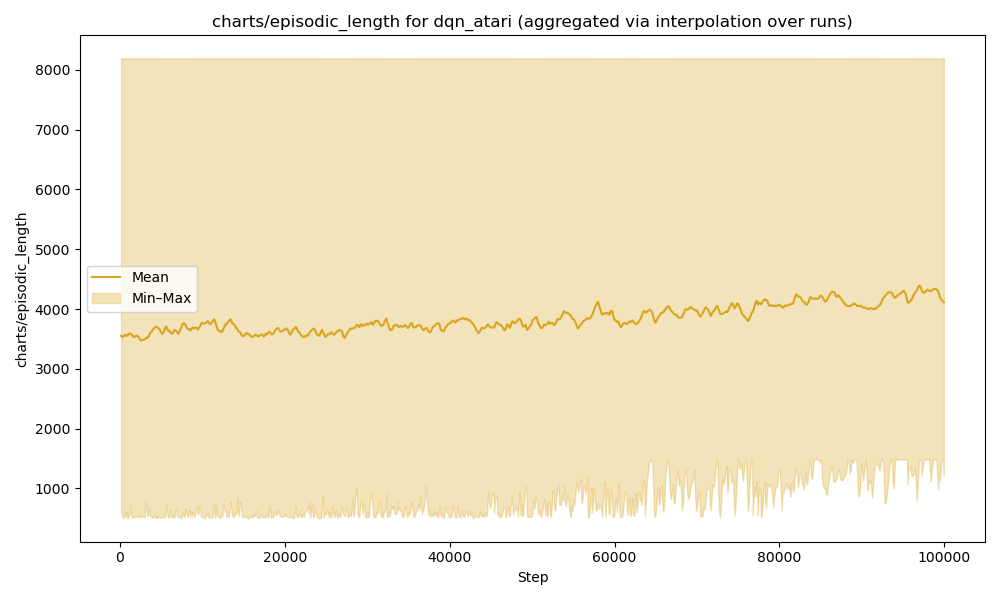
\includegraphics[width=.45\textwidth]{figures/dqn/charts_episodic_length_dqn_atari.png} \label{fig:dqn_episodic_length}} \quad
	\subfloat[][\emph{Steps per second (SPS) for DQN. After an initial ramp-up, 
		the mean SPS stabilizes around 170--180, 
		with some runs dipping as low as 20 or spiking above 200.}]
	{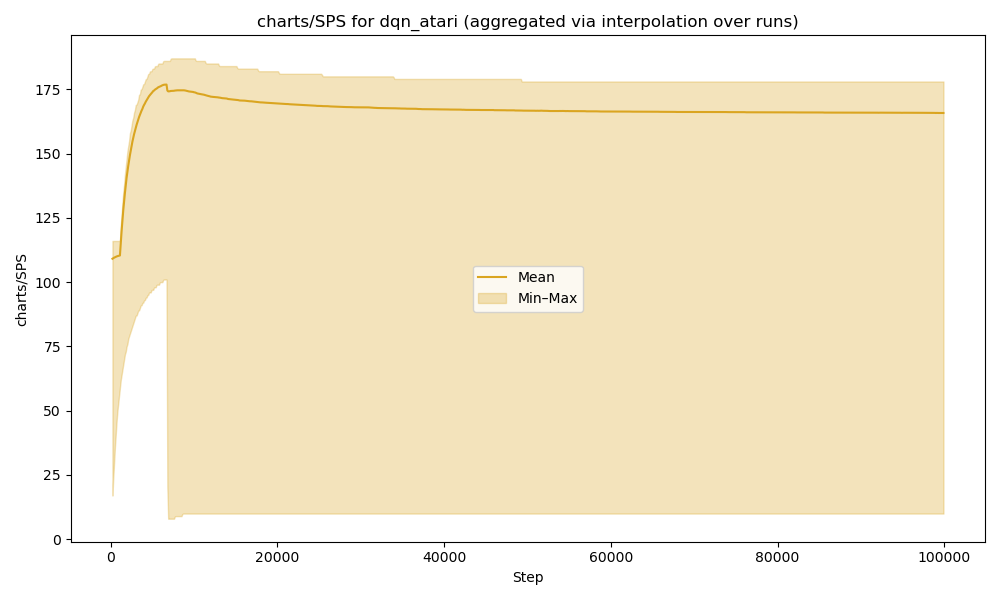
\includegraphics[width=.45\textwidth]{figures/dqn/charts_SPS_dqn_atari.png} \label{fig:dqn_sps}} \\ 
	\subfloat[][\emph{Estimated Q-values (\texttt{losses/q\_values}) for DQN 
		(aggregated over 32 runs). 
		The mean Q-value climbs from near 0 up to \(\sim\)4--5, 
		while some runs exceed 10.}]
	{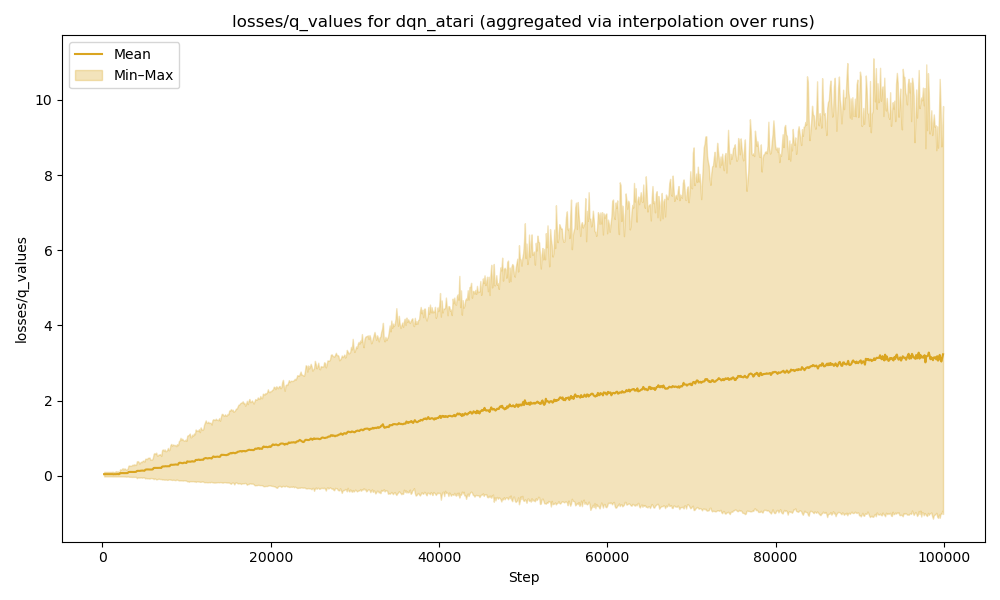
\includegraphics[width=.45\textwidth]{figures/dqn/losses_q_values_dqn_atari.png} \label{fig:dqn_q_values}} \quad
	\subfloat[][\emph{TD loss (\texttt{losses/td\_loss}) for DQN. 
		Losses grow with training, reaching above 3.0 in some runs, 
		reflecting substantial variance near the final stages.}]
	{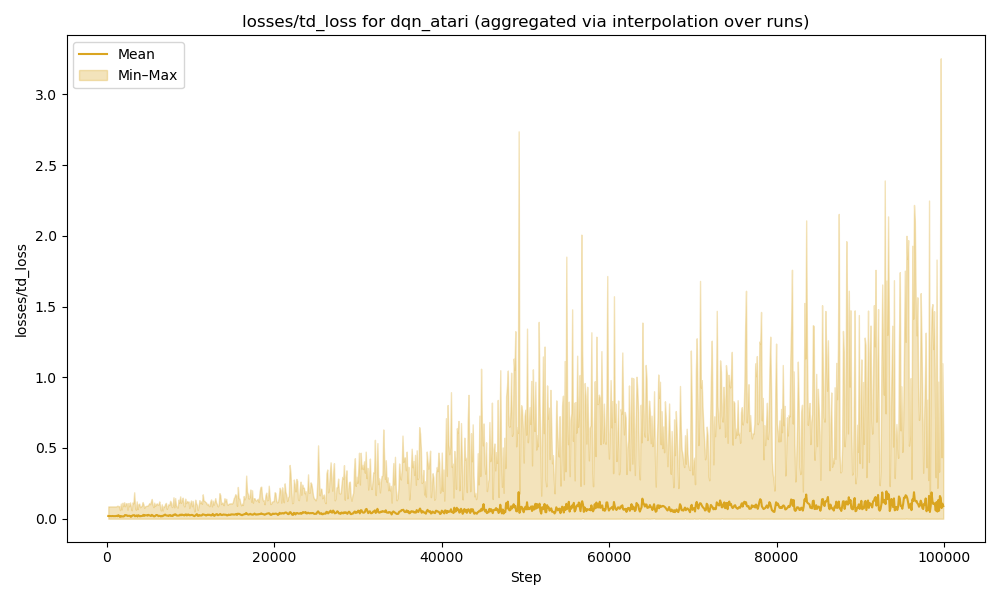
\includegraphics[width=.45\textwidth]{figures/dqn/losses_td_loss_dqn_atari.png} \label{fig:dqn_td_loss}}
	\caption{Performance metrics for DQN over 100k steps, aggregated across 32 runs.}
	\label{fig:dqn_subfigures}
\end{figure}

%
%\begin{figure}
%	\centering
%	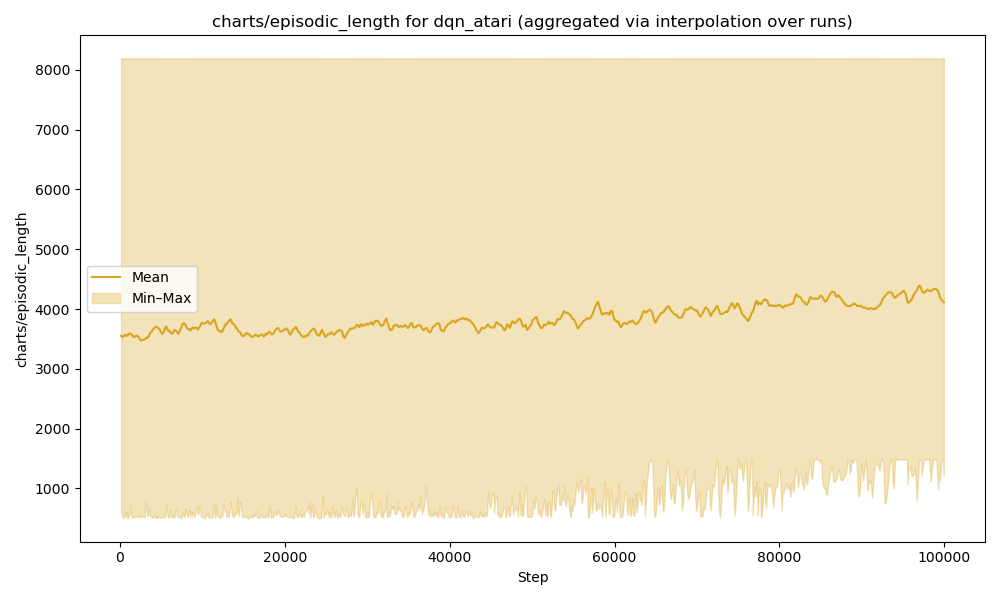
\includegraphics[width=0.6\textwidth]{figures/dqn/charts_episodic_length_dqn_atari.png}
%	\caption{Aggregated episodic length for DQN over 100k steps 
%		(interpolation across 32 runs). 
%		The mean hovers around 3500--4000 steps, 
%		while the min--max envelope extends from near 0 to over 8000.}
%	\label{fig:dqn_episodic_length}
%\end{figure}
%\begin{figure}
%	\centering
%	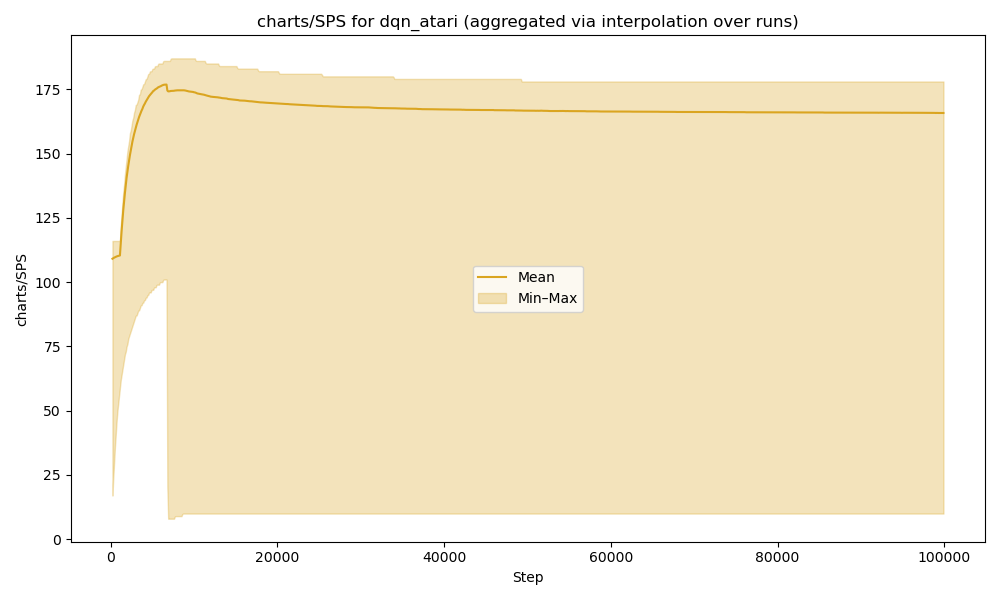
\includegraphics[width=0.6\textwidth]{figures/dqn/charts_SPS_dqn_atari.png}
%	\caption{Steps per second (SPS) for DQN. After an initial ramp-up, 
%		the mean SPS stabilizes around 170--180, 
%		with some runs dipping as low as 20 or spiking above 200.}
%	\label{fig:dqn_sps}
%\end{figure}
%\begin{figure}
%	\centering
%	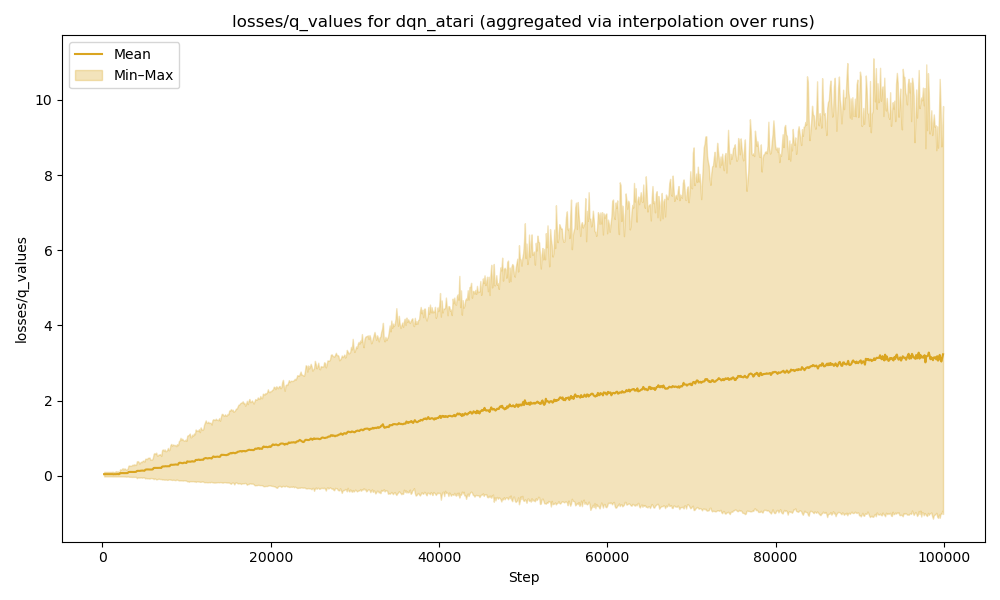
\includegraphics[width=0.6\textwidth]{figures/dqn/losses_q_values_dqn_atari.png}
%	\caption{Estimated Q-values (\texttt{losses/q\_values}) for DQN 
%		(aggregated over 32 runs). 
%		The mean Q-value climbs from near 0 up to \(\sim\)4--5, 
%		while some runs exceed 10.}
%	\label{fig:dqn_q_values}
%\end{figure}
%\begin{figure}
%	\centering
%	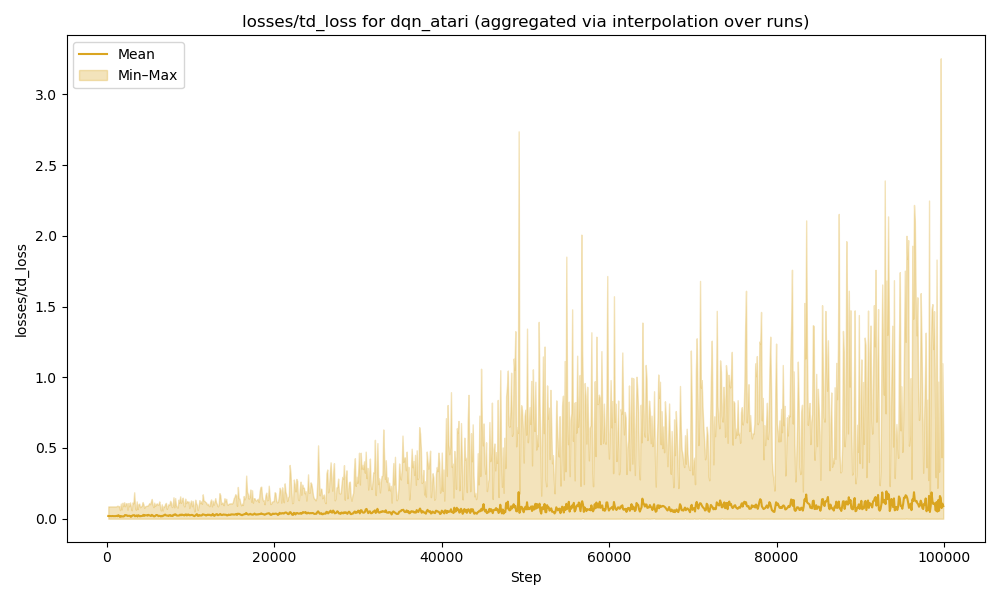
\includegraphics[width=0.6\textwidth]{figures/dqn/losses_td_loss_dqn_atari.png}
%	\caption{TD loss (\texttt{losses/td\_loss}) for DQN. 
%		Losses grow with training, reaching above 3.0 in some runs, 
%		reflecting substantial variance near the final stages.}
%	\label{fig:dqn_td_loss}
%\end{figure}

\paragraph{Q-Values and TD Loss}
Figures~\ref{fig:dqn_q_values} and \ref{fig:dqn_td_loss} show \texttt{losses/q\_values} and 
\texttt{losses/td\_loss}, respectively, across all runs.
On average, Q-values increase steadily, suggesting the network’s estimates 
of future returns keep growing with experience. However, 
the broad min--max band indicates some seeds or games diverge or plateau differently. 
The TD loss remains small in early training but spikes in certain runs, 
possibly due to volatile updates from the replay buffer once it’s partially filled.

\paragraph{Episodic Return (Human vs.\ Min--Max Normalized)}
We analyzed the collected episodic returns applying both the human normalization and min--max normalization schemes, as explained in section~\vref{subsubsec:normalization}.
Figures~\ref{fig:dqn_return_human} and \ref{fig:dqn_return_minmax} aggregate 
these returns across all 32 runs, while 
Figures~\ref{fig:dqn_return_pergame_human} and \ref{fig:dqn_return_pergame_minmax} 
show per-game curves.

\begin{figure}
	\centering
	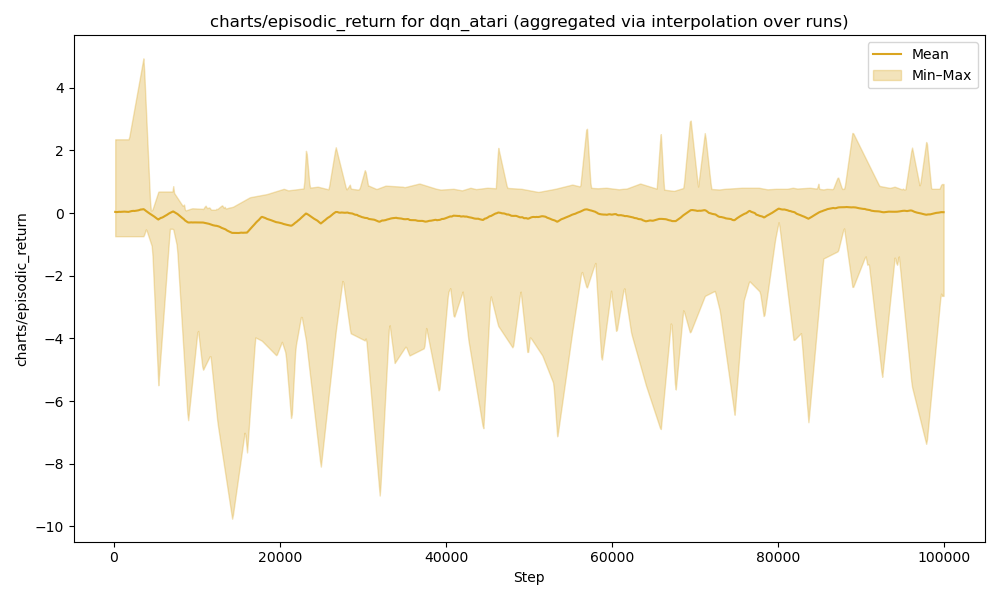
\includegraphics[width=0.6\textwidth]{figures/dqn/charts_episodic_return_human_dqn_atari.png}
	\caption{Aggregated DQN episodic return (human-normalized) 
		over 100k steps. The shaded region represents min--max variation.}
	\label{fig:dqn_return_human}
\end{figure}

\begin{figure}
	\centering
	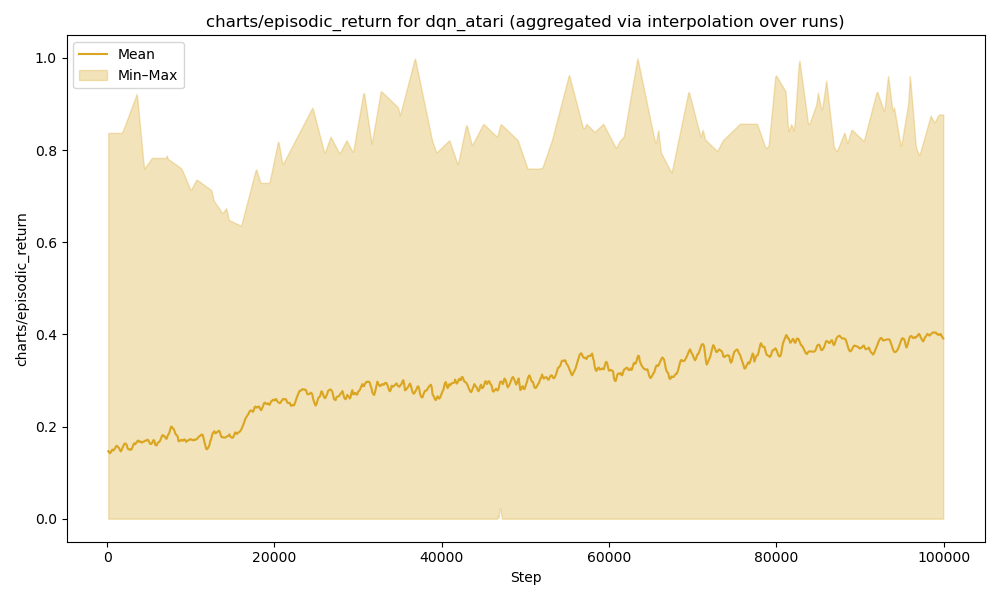
\includegraphics[width=0.6\textwidth]{figures/dqn/charts_episodic_return_minmax_dqn_atari.png}
	\caption{Aggregated DQN episodic return (min--max normalized).}
	\label{fig:dqn_return_minmax}
\end{figure}

In the human-normalized plot, the mean hovers near zero, 
occasionally dipping negative due to poor performance on certain games. 
In the min--max plot, the average climbs from near 0.2 to around 0.4--0.5 by the end, 
indicating moderate relative progress.

\begin{figure}
	\centering
	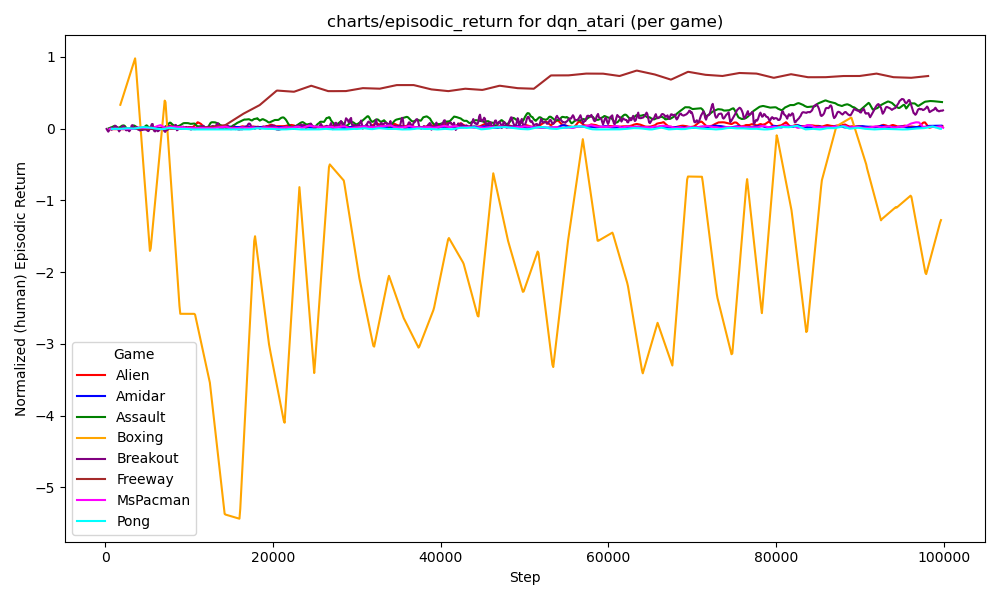
\includegraphics[width=0.6\textwidth]{figures/dqn/charts_episodic_return_per_game_human_dqn_atari.png}
	\caption{DQN returns (human-normalized) by game. Each line aggregates 
		four seeds for that specific environment.}
	\label{fig:dqn_return_pergame_human}
\end{figure}

\begin{figure}
	\centering
	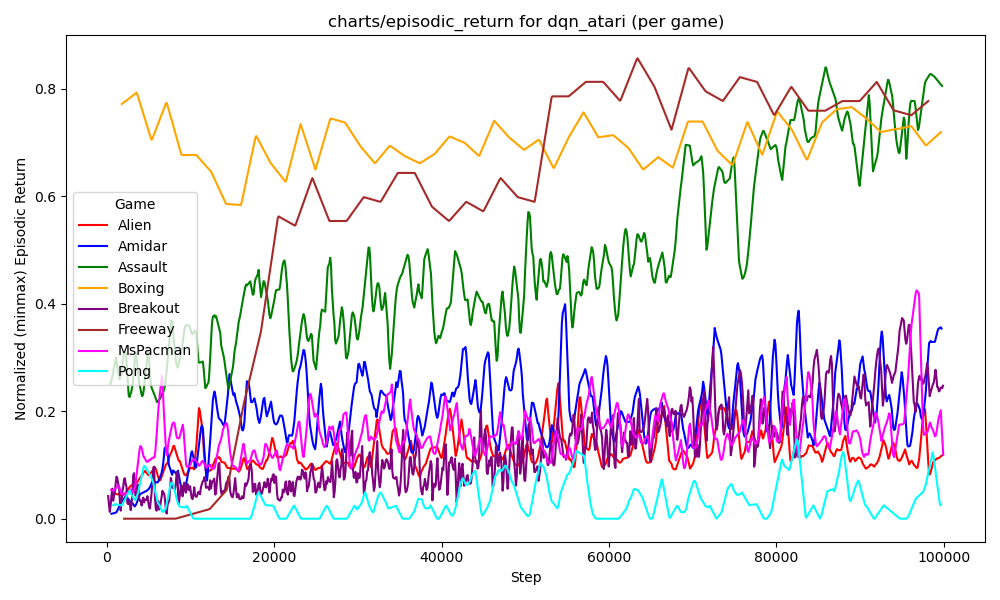
\includegraphics[width=0.6\textwidth]{figures/dqn/charts_episodic_return_per_game_minmax_dqn_atari.png}
	\caption{DQN returns (min--max normalized) by game.}
	\label{fig:dqn_return_pergame_minmax}
\end{figure}

Different environments see dramatically different results: 
\emph{Freeway} often approaches high normalized scores, while 
\emph{Pong} and \emph{MsPacman} remain relatively low 
(especially in the human-normalized scale).

\paragraph{Emissions}
Table~\ref{tab:dqn_emissions} presents the aggregated CO\textsubscript{2}-eq for DQN 
(over all 32 runs). The mean is about \(\textbf{0.00647 kg}\), 
with a minimum of 0.00616 and a maximum near 0.0070.

\begin{table}
	\caption{Carbon emissions (kg\,CO\textsubscript{2}eq) for DQN across 32 runs.}
	\label{tab:dqn_emissions}
	\centering
	\makebox[\textwidth]{%
	\begin{tabularx}{1.1\textwidth}{lXXXXXXXX}
		\toprule
		\textbf{Algorithm} & \textbf{mean} & \textbf{std} & \textbf{median} & 
		\textbf{q25} & \textbf{q75} & \textbf{min} & \textbf{max} & \textbf{iqmean} \\
		\midrule
		DQN & 0.006469 & 0.0002609 & 0.006342 & 0.006296 & 0.006578 & 0.006162 & 0.006997 & 0.006369 \\
		\bottomrule
	\end{tabularx}
	}
\end{table}

\paragraph{Evaluation Results}
Table~\ref{tab:dqn_eval_overall} aggregates final human-/min--max-normalized 
returns \emph{over all 32 runs}. A game-by-game breakdown 
(Table~\ref{tab:dqn_eval_gamewise}) highlights large variability: 
\emph{Freeway} can exceed 0.7 (human norm) or 0.75 (min--max), 
while \emph{Boxing} sees a wide range from $-5$ to nearly $+5$ in human norm.

\begin{table}
	\caption{Overall final evaluation (10 episodes each) for DQN across all runs.}
	\label{tab:dqn_eval_overall}
	\centering
	\begin{tabular}{lcccccccc}
		\toprule
		\textbf{Normalization} & \textbf{mean} & \textbf{std} & \textbf{median} & 
		\textbf{q25} & \textbf{q75} & \textbf{min} & \textbf{max} & \textbf{iqmean} \\
		\midrule
		\textbf{Human} & 0.1353 & 0.7541 & 0.0338 & 0.00072 & 0.398 & -5.024 & 4.738 & 0.1137 \\
		\textbf{Min--Max} & 0.3802 & 0.3099 & 0.2899 & 0.0969 & 0.7143 & 0.0 & 0.9881 & 0.3426 \\
		\bottomrule
	\end{tabular}
\end{table}

\begin{table}
	\caption{Per-game final evaluation for DQN (human- vs.\ min--max normalized). 
		Each cell aggregates 10 episodes $\times$ 4 seeds = 40 total episodes in that game.}
	\label{tab:dqn_eval_gamewise}
	\centering
	\begin{tabular}{llcccc}
		\toprule
		\textbf{Game} & \textbf{Norm} & \textbf{mean} & \textbf{std} & \textbf{min} & \textbf{max}\\
		\midrule
		Alien    & Human   & 0.0624 & 0.0752 & 0.0048 & 0.2636 \\
		    & Min--Max & 0.1607 & 0.1250 & 0.0650 & 0.4950 \\
		\cmidrule{1-6}
		Amidar   & Human   & 0.0226 & 0.0138 & 0.00072 & 0.0450 \\
		   & Min--Max & 0.2005 & 0.1065 & 0.0323 & 0.3733 \\
		\cmidrule{1-6}
		Assault  & Human   & 0.3167 & 0.1120 & -0.0262 & 0.4920 \\
		  & Min--Max & 0.7216 & 0.1703 & 0.2005 & 0.9881 \\
		\cmidrule{1-6}
		Boxing   & Human   & -0.4167 & 1.9504 & -5.0238 & 4.7381 \\
		   & Min--Max & 0.7469 & 0.0635 & 0.5969 & 0.9147 \\
		\cmidrule{1-6}
		Breakout & Human   & 0.3796 & 0.1246 & 0.1096 & 0.6080 \\
		 & Min--Max & 0.3454 & 0.0987 & 0.1316 & 0.5263 \\
		\cmidrule{1-6}
		Freeway  & Human   & 0.7162 & 0.0589 & 0.6419 & 0.8784 \\
		  & Min--Max & 0.7571 & 0.0622 & 0.6786 & 0.9286 \\
		\cmidrule{1-6}
		MsPacman & Human   & 0.0099 & 0.0120 & -0.0076 & 0.0262 \\
		 & Min--Max & 0.1047 & 0.0484 & 0.0340 & 0.1702 \\
		\cmidrule{1-6}
		Pong     & Human   & -0.0083 & 0.0074 & -0.01 & 0.0233 \\
		     & Min--Max & 0.0050 & 0.0221 & 0.0 & 0.1 \\
		\bottomrule
	\end{tabular}
\end{table}

\paragraph{Observations}
In summary:
\begin{itemize}
	\item \textbf{Episodic length} stabilizes around 3500--4000 steps on average, 
	with some extreme runs either terminating quickly or persisting up to 8000 steps.
	\item \textbf{SPS} quickly rises to around 170--180, illustrating the efficiency 
	of the implementation (though some runs are slower).
	\item \textbf{Q-values and TD loss} both exhibit broad variability. On average, 
	Q-values climb steadily to 4--5, but certain runs exceed 10. The TD loss 
	can spike above 3 for some seeds, indicating unstable updates.
	\item \textbf{Returns} show moderate success on easier tasks like \textit{Freeway} 
	and \textit{Boxing}, but remain low in \textit{Pong} or \textit{MsPacman}. Overall, 
	min--max mean is about 0.38, whereas human-normalized is only 0.14 (due in part 
	to highly negative outliers on certain seeds).
	\item \textbf{Emissions} remain modest, at about 0.00647\,kg CO\textsubscript{2}-eq 
	per run. This is unsurprising for a 100k-step budget, but still notable for 
	comparing across algorithms in subsequent sections.
\end{itemize}

DQN thus provides a baseline—relatively simple and lightweight—to which we will 
compare Double DQN, Prioritized Experience Replay, Dueling DQN, and C51 
in the next subsections, evaluating whether each extension justifies 
its additional complexity and energy usage.


\subsubsection{Double DQN}
\label{subsubsec:double_dqn}

\paragraph{(Hyper)Parameters}
Table~\ref{tab:ddqn_hyperparams} shows the main hyperparameters used in our Double DQN implementation.  
As with the baseline DQN (Section~\ref{subsubsec:dqn_baseline}), \texttt{env\_id} and \texttt{seed} vary across the 32 runs (eight Atari games $\times$ four seeds), while the rest remain unchanged. In particular, we again set \texttt{buffer\_size}=10k and \texttt{learning\_starts}=1000. 
The Double DQN update rule differs from standard DQN by separately selecting the action and evaluating its value, aiming to reduce the maximization bias that arises from using the same values to both choose and evaluate an action.

\begin{table}
	\caption{Key hyperparameters for Double DQN. Only \texttt{env\_id} and \texttt{seed} change across runs.}
	\label{tab:ddqn_hyperparams}
	\centering
	\begin{tabular}{ll}
		\toprule
		\textbf{Parameter} & \textbf{Value} \\
		\midrule
		\texttt{exp\_name}                & ddqn\_atari \\
		\texttt{seed}                     & 1..4 \\
		\texttt{torch\_deterministic}     & True \\
		\texttt{cuda}                     & True \\
		\texttt{track}                    & True \\
		\texttt{wandb\_project\_name}     & rlsb \\
		\texttt{capture\_video}           & False \\
		\texttt{save\_model}              & True \\
		\texttt{upload\_model}            & False \\
		\texttt{env\_id}                  & e.g.\ AlienNoFrameskip-v4 \\
		\texttt{total\_timesteps}         & 100000 \\
		\texttt{learning\_rate}           & 0.0001 \\
		\texttt{num\_envs}                & 1 \\
		\texttt{buffer\_size}             & 10000 \\
		\texttt{gamma}                    & 0.99 \\
		\texttt{tau}                      & 1.0 \\
		\texttt{target\_network\_frequency} & 1000 \\
		\texttt{batch\_size}             & 32 \\
		\texttt{start\_e}, \texttt{end\_e} & 1.0 $\to$ 0.01 \\
		\texttt{exploration\_fraction}    & 0.1 \\
		\texttt{learning\_starts}         & 1000 \\
		\texttt{train\_frequency}         & 4 \\
		\bottomrule
	\end{tabular}
\end{table}

\paragraph{Hyperparameter Tuning}
To isolate the effect of Double DQN, we kept all settings identical to the baseline DQN, simply enabling the Double DQN update scheme. 
Following~\cite{van:double_q}, we tested a higher \texttt{target\_network\_frequency} (e.g.\ 3000, scaled from the 10k--20k range in the original paper), but at 100k steps, performance was comparable or slightly better with 1000, so we retained the lower frequency. 

\paragraph{Training Dynamics (Aggregated Over 32 Runs)}
Figure~\ref{fig:ddqn_subfigs} presents key metrics—episodic length, steps per second (SPS), estimated Q-values, and TD loss—aggregated across 32 runs (eight games, four seeds each). 

\begin{figure}
	\centering
	\subfloat[][Episodic length (\texttt{charts\_episodic\_length}). 
	The mean sits around 3500--4000 steps, 
	min--max ranges from near 0 up to 8000.]{
		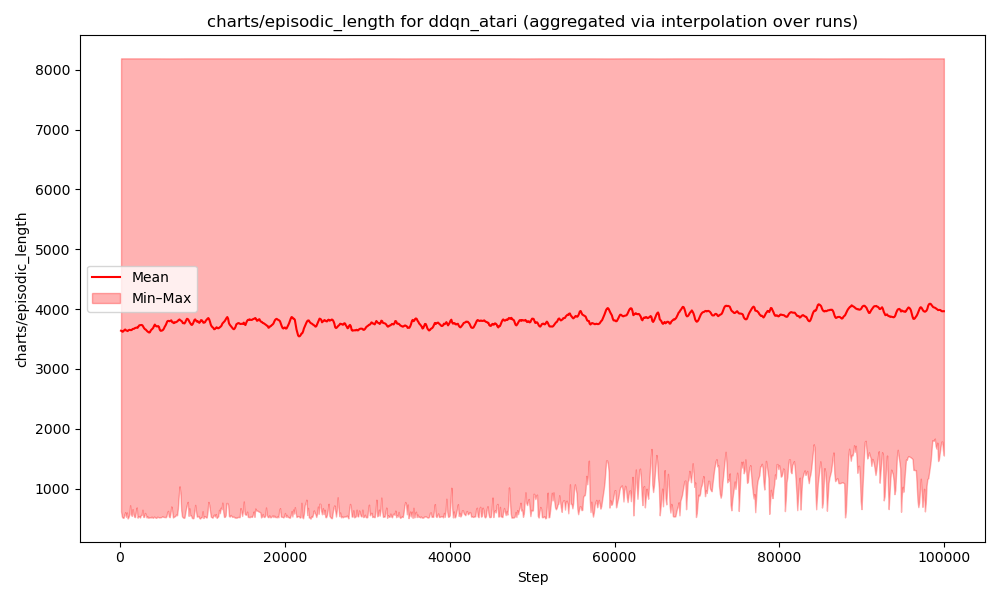
\includegraphics[width=.45\textwidth]{figures/ddqn/charts_episodic_length_ddqn_atari.png}
		\label{fig:ddqn_episodic_length}
	}
	\quad
	\subfloat[][Steps per second (SPS). After an initial climb near 180, 
	the mean gradually settles around 165--170.]{
		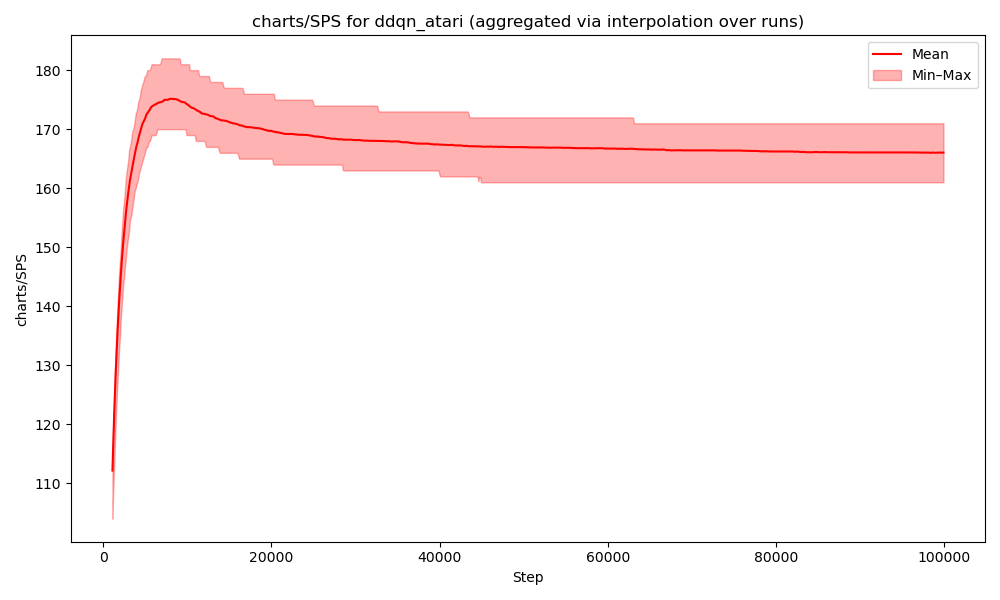
\includegraphics[width=.45\textwidth]{figures/ddqn/charts_SPS_ddqn_atari.png}
		\label{fig:ddqn_sps}
	}
	\\[1em]
	\subfloat[][Estimated Q-values (\texttt{losses/q\_values}). 
	The mean climbs from 0 to about 2--3, 
	with upper outliers above 6.]{
		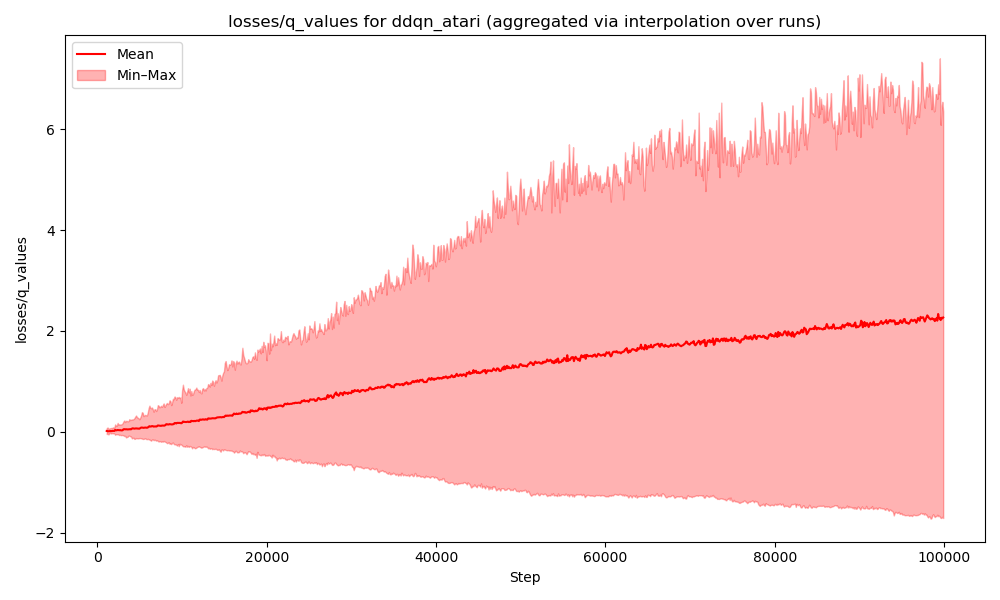
\includegraphics[width=.45\textwidth]{figures/ddqn/losses_q_values_ddqn_atari.png}
		\label{fig:ddqn_q_values}
	}
	\quad
	\subfloat[][TD loss (\texttt{losses/td\_loss}). 
	Occasional spikes above 2.0 reflect instability on certain seeds.]{
		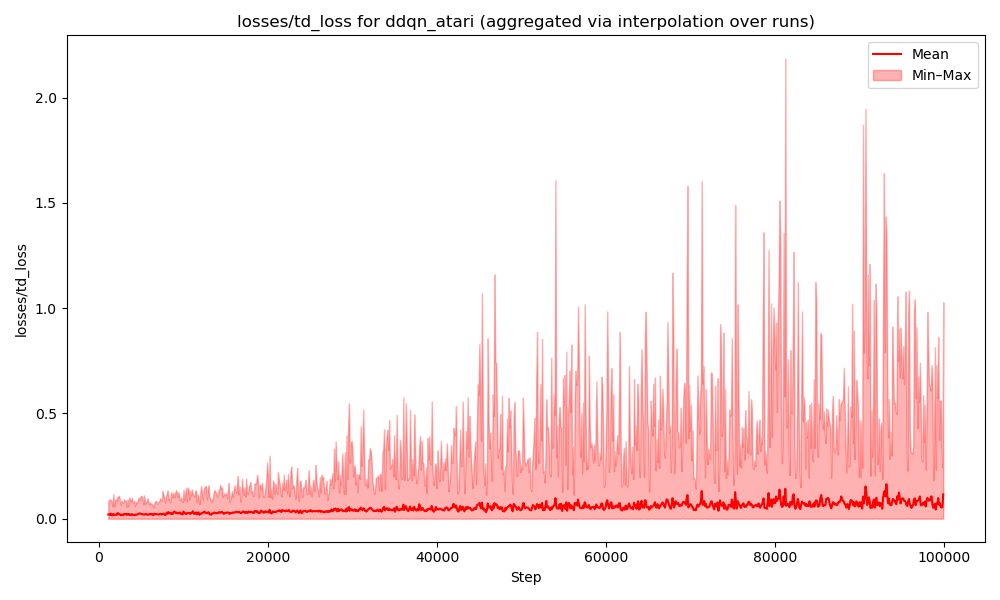
\includegraphics[width=.45\textwidth]{figures/ddqn/losses_td_loss_ddqn_atari.png}
		\label{fig:ddqn_td_loss}
	}
	\caption{Double DQN training metrics over 100k steps, aggregated over 32 runs.}
	\label{fig:ddqn_subfigs}
\end{figure}

Episodic length and SPS curves are very similar to baseline DQN’s (Section~\ref{subsubsec:dqn_baseline}). 
Meanwhile, the mean Q-values grow more modestly than DQN’s (which often exceed 4--5 by the end), suggesting 
Double DQN’s approach does mitigate overestimation somewhat. 
TD loss remains low overall, though some runs spike above 2.0 near late training.

\paragraph{Episodic Return (Human vs.\ Min--Max Normalized)}
Figures~\ref{fig:ddqn_return_human} and \ref{fig:ddqn_return_minmax} show Double DQN’s aggregated episodic returns (human- and min--max-normalized, respectively). 
Figures~\ref{fig:ddqn_return_pergame_human} and \ref{fig:ddqn_return_pergame_minmax} break these results down by game.

\begin{figure}
	\centering
	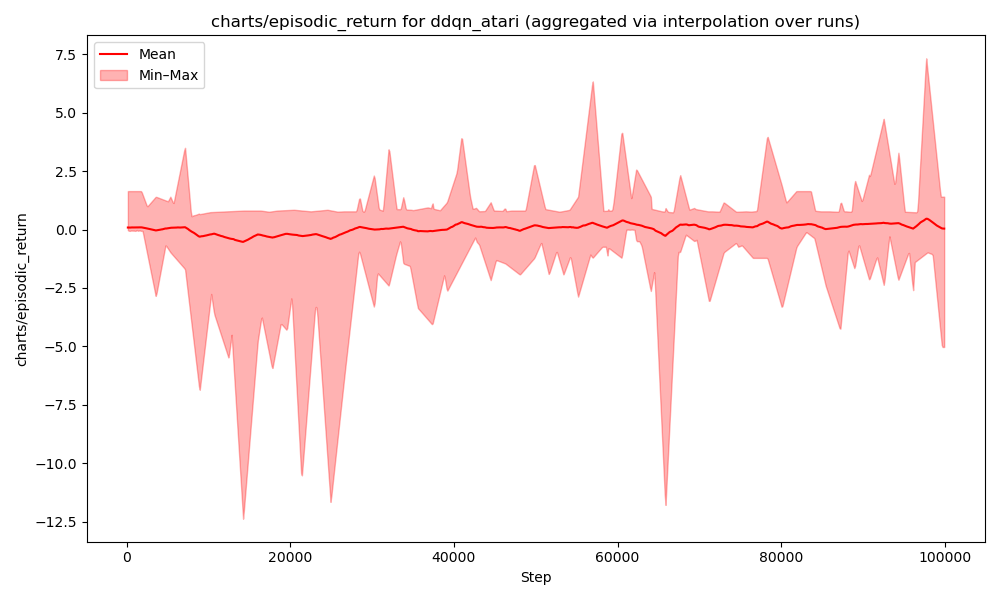
\includegraphics[width=0.6\textwidth]{figures/ddqn/charts_episodic_return_human_ddqn_atari.png}
	\caption{Double DQN episodic return (human-normalized), aggregated across 32 runs.}
	\label{fig:ddqn_return_human}
\end{figure}

\begin{figure}
	\centering
	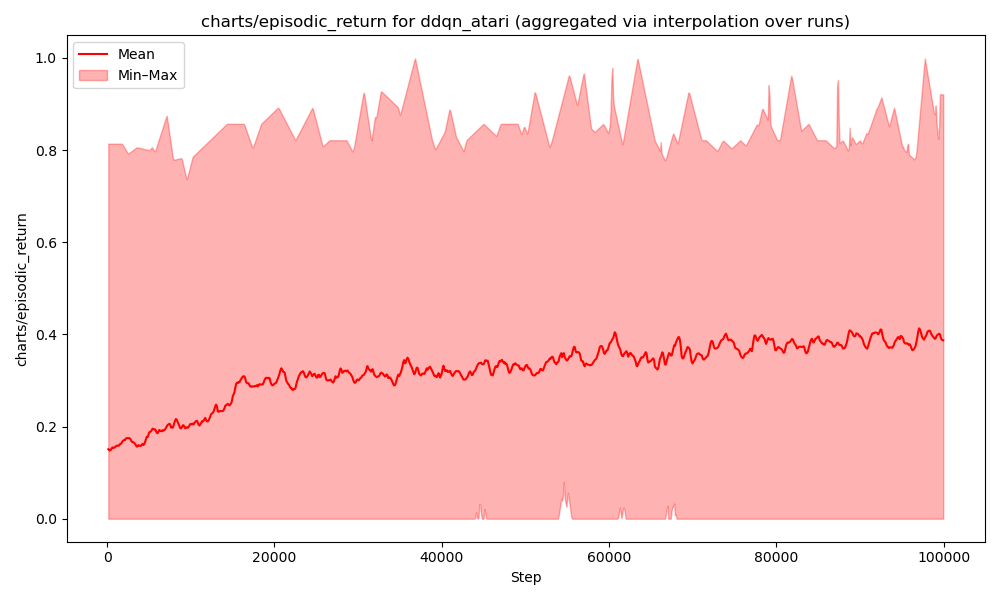
\includegraphics[width=0.6\textwidth]{figures/ddqn/charts_episodic_return_minmax_ddqn_atari.png}
	\caption{Double DQN episodic return (min--max normalized), aggregated across 32 runs.}
	\label{fig:ddqn_return_minmax}
\end{figure}

\begin{figure}
	\centering
	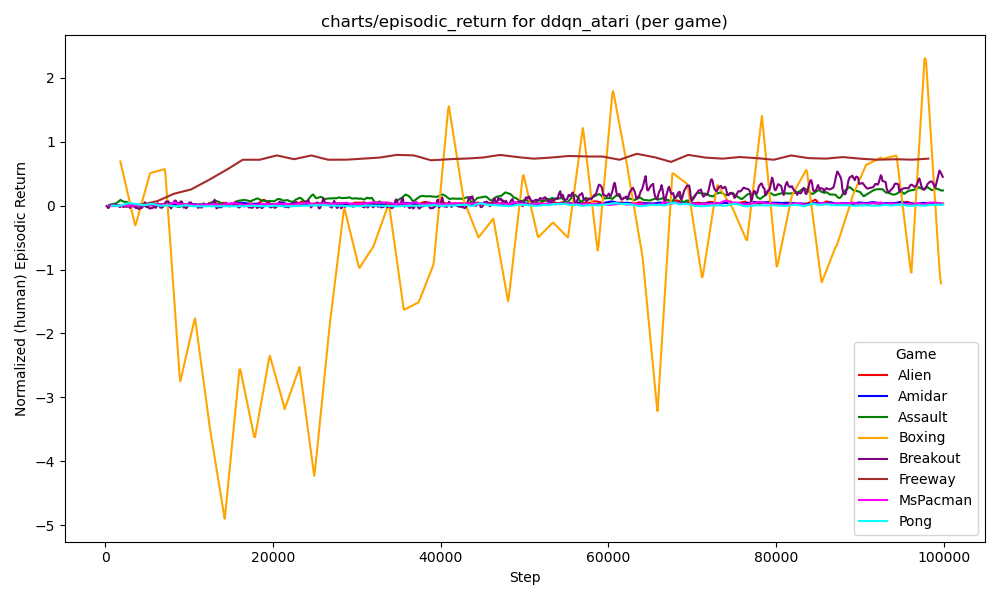
\includegraphics[width=0.6\textwidth]{figures/ddqn/charts_episodic_return_per_game_human_ddqn_atari.png}
	\caption{Double DQN returns per game (human-normalized). 
		Some large negative dips occur in \emph{Boxing}, 
		while \emph{Freeway} remains relatively high.}
	\label{fig:ddqn_return_pergame_human}
\end{figure}

\begin{figure}
	\centering
	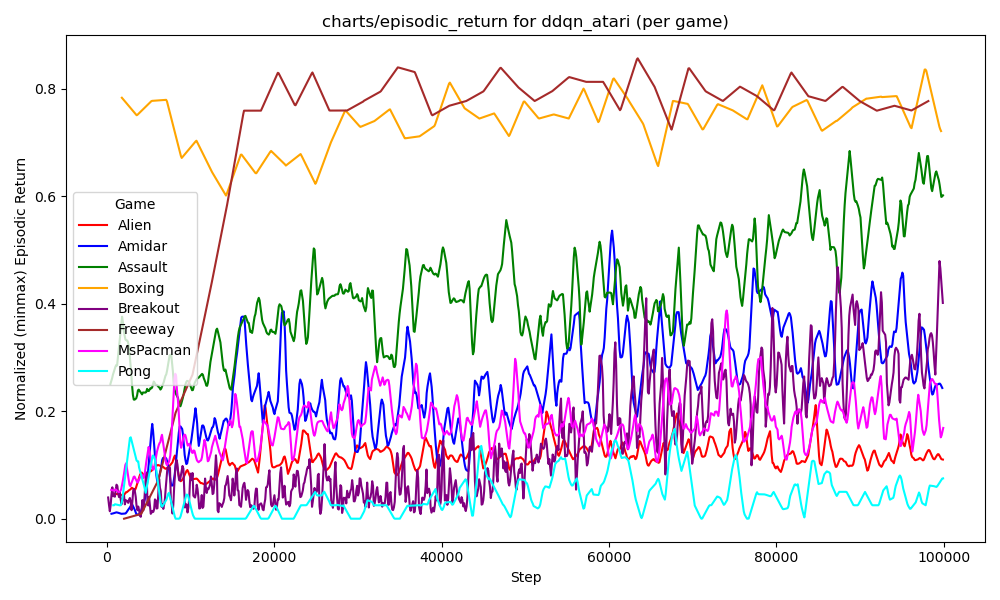
\includegraphics[width=0.6\textwidth]{figures/ddqn/charts_episodic_return_per_game_minmax_ddqn_atari.png}
	\caption{Double DQN returns per game (min--max normalized).}
	\label{fig:ddqn_return_pergame_minmax}
\end{figure}

As in the baseline, \emph{Freeway} can achieve near 0.7--0.8 in human norm, 
while \emph{Boxing} causes occasional highly negative runs. 
Min--max normalized returns rise from $\sim 0.2$ to $\sim 0.4$, 
similar to DQN’s overall trajectory.

\paragraph{Emissions}
Table~\ref{tab:ddqn_emissions} summarizes Double DQN’s CO\textsubscript{2}-eq emissions across 32 runs. 
The mean is about \textbf{0.00667\,kg}, slightly above DQN’s \(\sim 0.00647\).

\begin{table}
	\caption{Carbon emissions (kg\,CO\textsubscript{2}eq) for Double DQN, aggregated over 32 runs.}
	\label{tab:ddqn_emissions}
	\centering
	\makebox[\textwidth]{%
	\begin{tabularx}{1.1\textwidth}{lXXXXXXXX}
		\toprule
		\textbf{Algorithm} & \textbf{mean} & \textbf{std} & \textbf{median} & 
		\textbf{q25} & \textbf{q75} & \textbf{min} & \textbf{max} & \textbf{iqmean} \\
		\midrule
		Double DQN & 0.006672 & 0.000282 & 0.006549 & 0.006477 & 0.006755 
		& 0.006377 & 0.007267 & 0.006565 \\
		\bottomrule
	\end{tabularx}
	}
\end{table}

\paragraph{Evaluation Results}
Table~\ref{tab:ddqn_eval_overall} compiles final returns (human-/min--max normalization) aggregated over the 32 runs. 
Compared to DQN’s \(\sim\!0.135\) (human) and \(\sim\!0.380\) (min--max), Double DQN attains 0.023 (human) and 0.374 (min--max). 
While the min--max average is comparable, the human-normalized mean is noticeably lower due to substantial negative outliers (again, notably \emph{Boxing}).

\begin{table}
	\caption{Overall final evaluation (10 episodes each) for Double DQN across 32 runs.}
	\label{tab:ddqn_eval_overall}
	\centering
	\makebox[\textwidth]{%
	\begin{tabularx}{1.1\textwidth}{lXXXXXXXX}
		\toprule
		\textbf{Normalization} & \textbf{mean} & \textbf{std} & \textbf{median} & 
		\textbf{q25} & \textbf{q75} & \textbf{min} & \textbf{max} & \textbf{iqmean} \\
		\midrule
		\textbf{Human} & 0.0226 & 1.0083 & 0.0527 & 0.0127 & 0.2871 & -8.5952 & 2.5952 & 0.0894 \\
		\textbf{Min--Max} & 0.3737 & 0.2854 & 0.2887 & 0.1244 & 0.7054 & 0.0 & 1.0 & 0.3272 \\
		\bottomrule
	\end{tabularx}
	}
\end{table}

Table~\ref{tab:ddqn_eval_gamewise} shows the game-by-game breakdown, indicating \emph{Boxing} yields a min of -8.5952 and max of 2.5952 in human-normalized scale, dragging down the overall mean. Meanwhile, \emph{Freeway} remains consistently high.

\begin{table}
	\caption{Per-game final evaluation for Double DQN (human- vs.\ min--max normalized). 
		Each row aggregates 40 total episodes (10 per seed).}
	\label{tab:ddqn_eval_gamewise}
	\centering
	\begin{tabular}{llcccc}
		\toprule
		\textbf{Game} & \textbf{Norm} & \textbf{mean} & \textbf{std} & \textbf{min} & \textbf{max}\\
		\midrule
		Alien    & Human   & 0.0514 & 0.0340 & 0.0094 & 0.1327 \\
		& Min--Max & 0.1424 & 0.0565 & 0.0725 & 0.2775 \\
		\cmidrule{1-6}
		Amidar   & Human   & 0.0320 & 0.0222 & 0.0127 & 0.0953 \\
		& Min--Max & 0.2729 & 0.1708 & 0.1244 & 0.7604 \\
		\cmidrule{1-6}
		Assault  & Human   & 0.2310 & 0.1071 & -0.0427 & 0.4103 \\
		& Min--Max & 0.5913 & 0.1628 & 0.1754 & 0.8640 \\
		\cmidrule{1-6}
		Boxing   & Human   & -1.1607 & 2.4963 & -8.5952 & 2.5952 \\
		& Min--Max & 0.7227 & 0.0813 & 0.4806 & 0.8450 \\
		\cmidrule{1-6}
		Breakout & Human   & 0.2666 & 0.1470 & 0.0764 & 0.8738 \\
		& Min--Max & 0.2559 & 0.1165 & 0.1053 & 0.7368 \\
		\cmidrule{1-6}
		Freeway  & Human   & 0.7213 & 0.0493 & 0.6419 & 0.8784 \\
		& Min--Max & 0.7625 & 0.0521 & 0.6786 & 0.9286 \\
		\cmidrule{1-6}
		MsPacman & Human   & 0.0291 & 0.0245 & -0.0037 & 0.0730 \\
		& Min--Max & 0.1820 & 0.0986 & 0.0497 & 0.3586 \\
		\cmidrule{1-6}
		Pong     & Human   & 0.0100 & 0.0559 & -0.01 & 0.3233 \\
		& Min--Max & 0.0600 & 0.1676 & 0.0   & 1.0 \\
		\bottomrule
	\end{tabular}
\end{table}

\paragraph{Comparison with Baseline DQN}
Beyond the final statistics, we can compare Q-values and TD loss directly via overlapping curves. Figure~\vref{fig:dqn_vs_ddqn_qvalues} shows the \texttt{losses/q\_values} for both algorithms, with \texttt{ddqn\_atari} in red and \texttt{dqn\_atari} in gold; Double DQN’s mean Q-values grow more slowly, suggesting less overestimation. Figure~\vref{fig:dqn_vs_ddqn_td_loss} indicates TD loss remains similarly small for both, though DQN occasionally spikes higher. The barplot in figure~\ref{fig:emissions_dqn_ddqn} shows the mean emissions side-by-side.

\begin{figure}
	\centering
	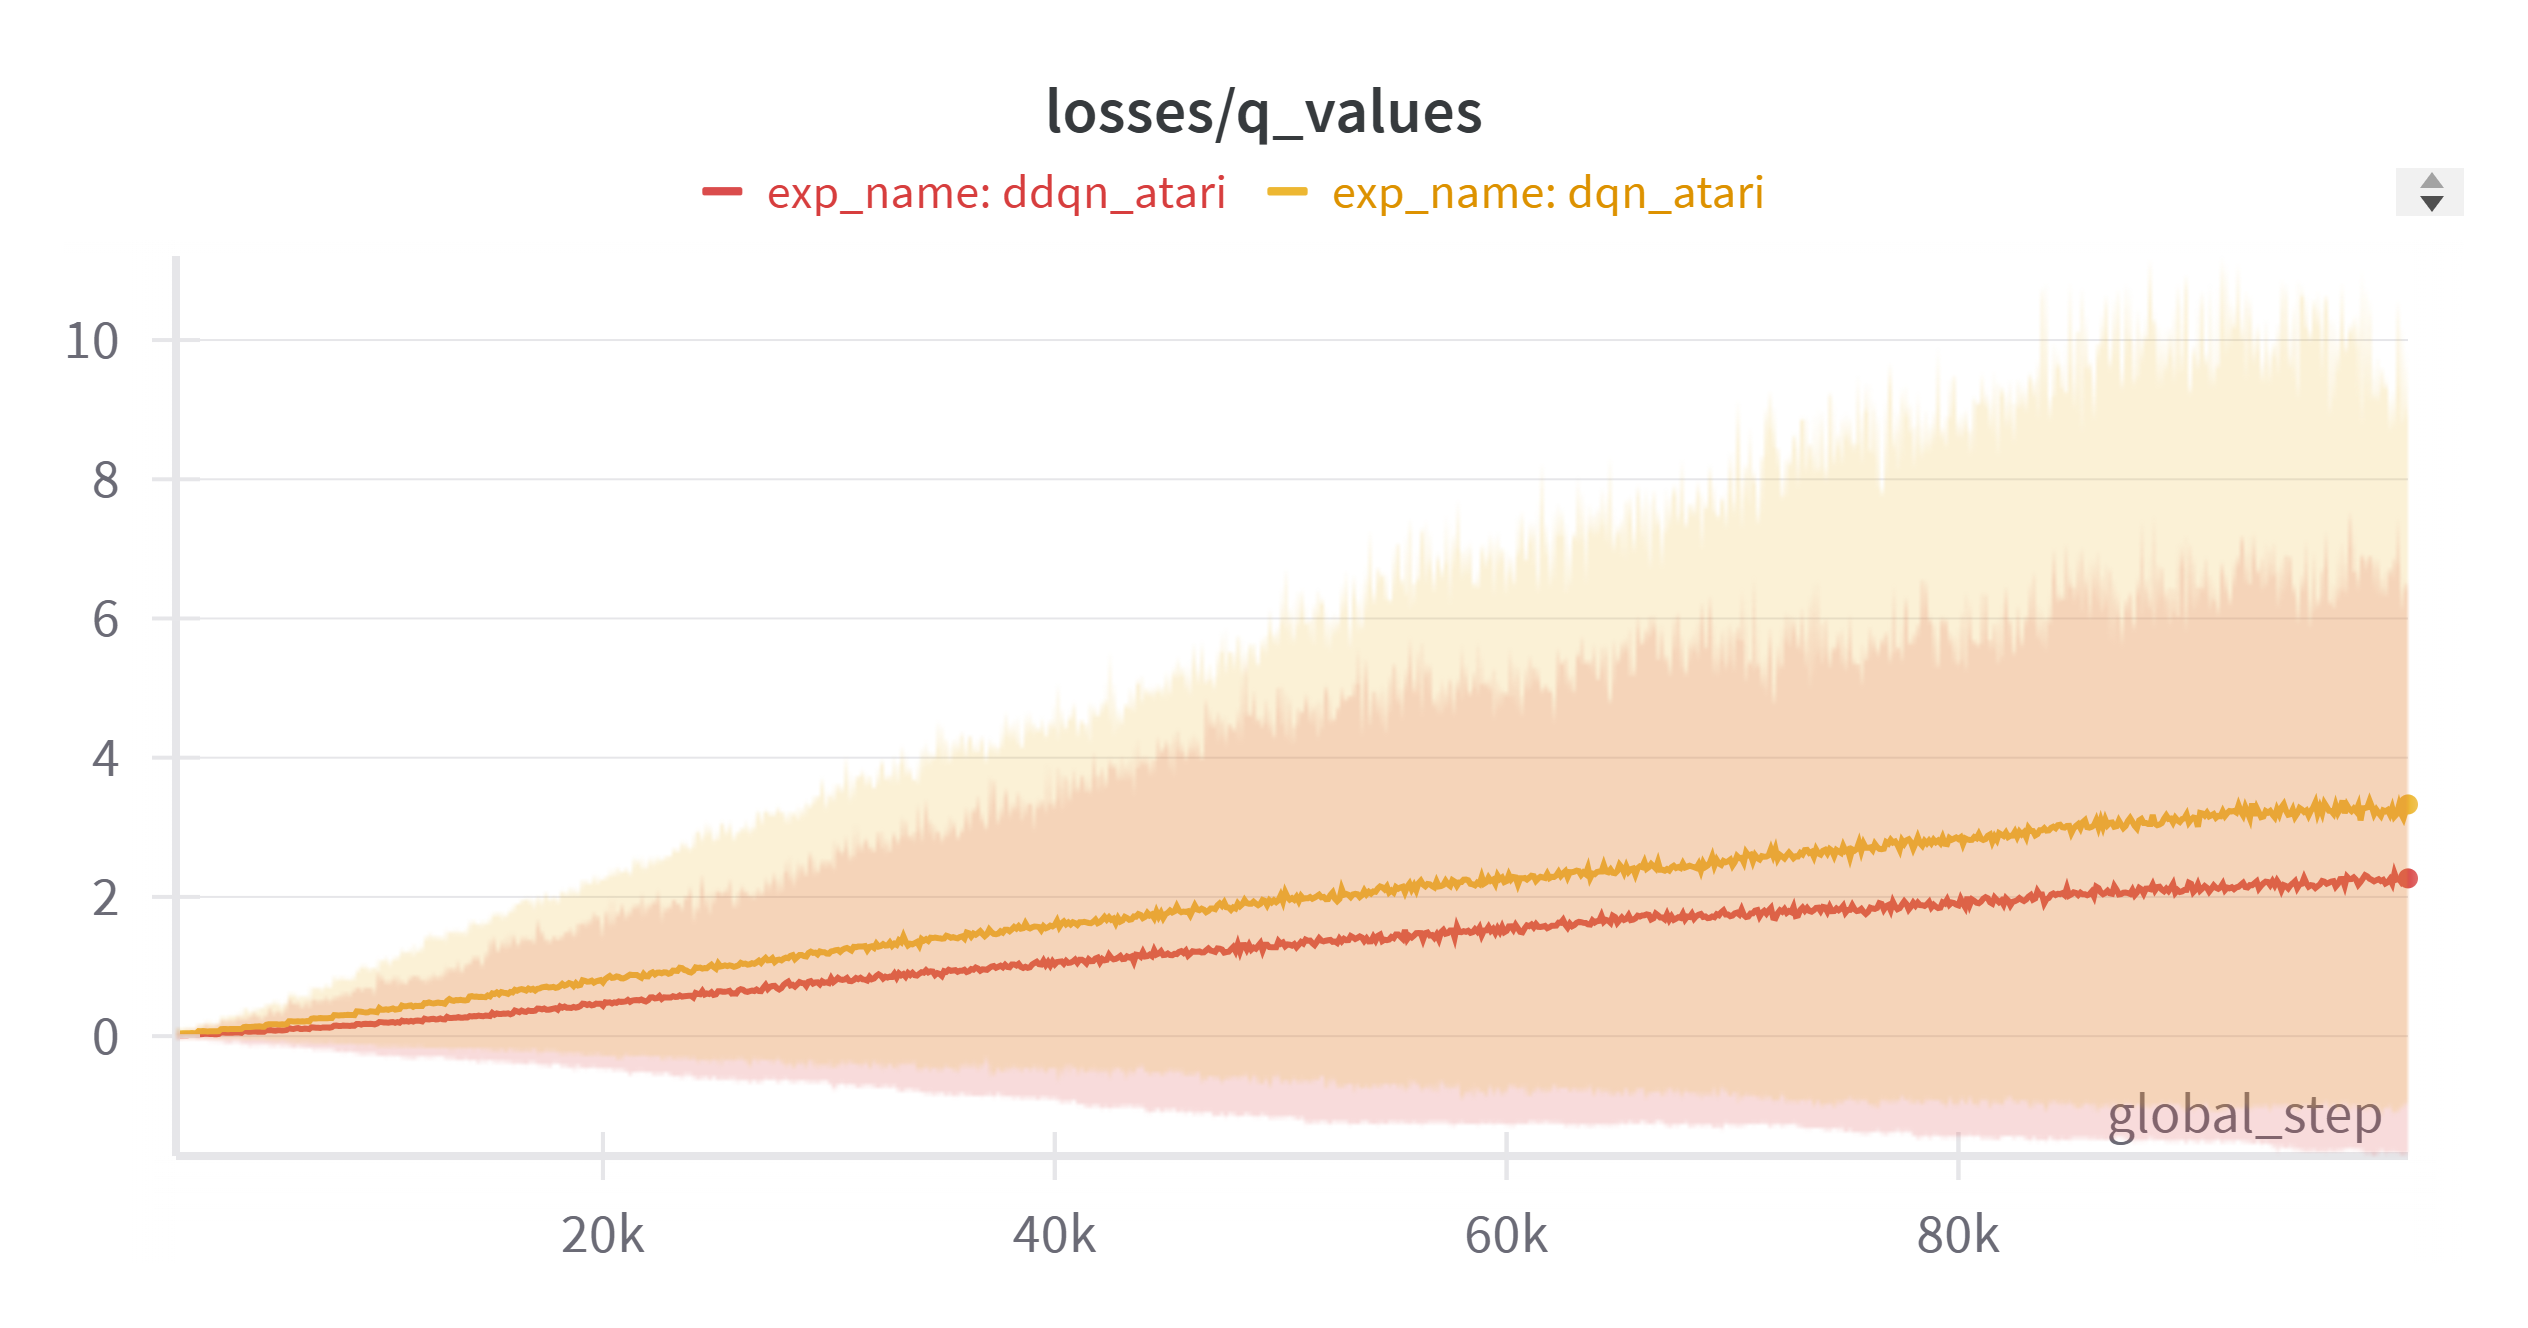
\includegraphics[width=0.6\textwidth]{figures/ddqn/comparison_losses_q_values_dqn_ddqn.png}
	\caption{Comparison of mean Q-values (with min--max shading) for DQN (gold) vs.\ Double DQN (red).}
	\label{fig:dqn_vs_ddqn_qvalues}
\end{figure}

\begin{figure}
	\centering
	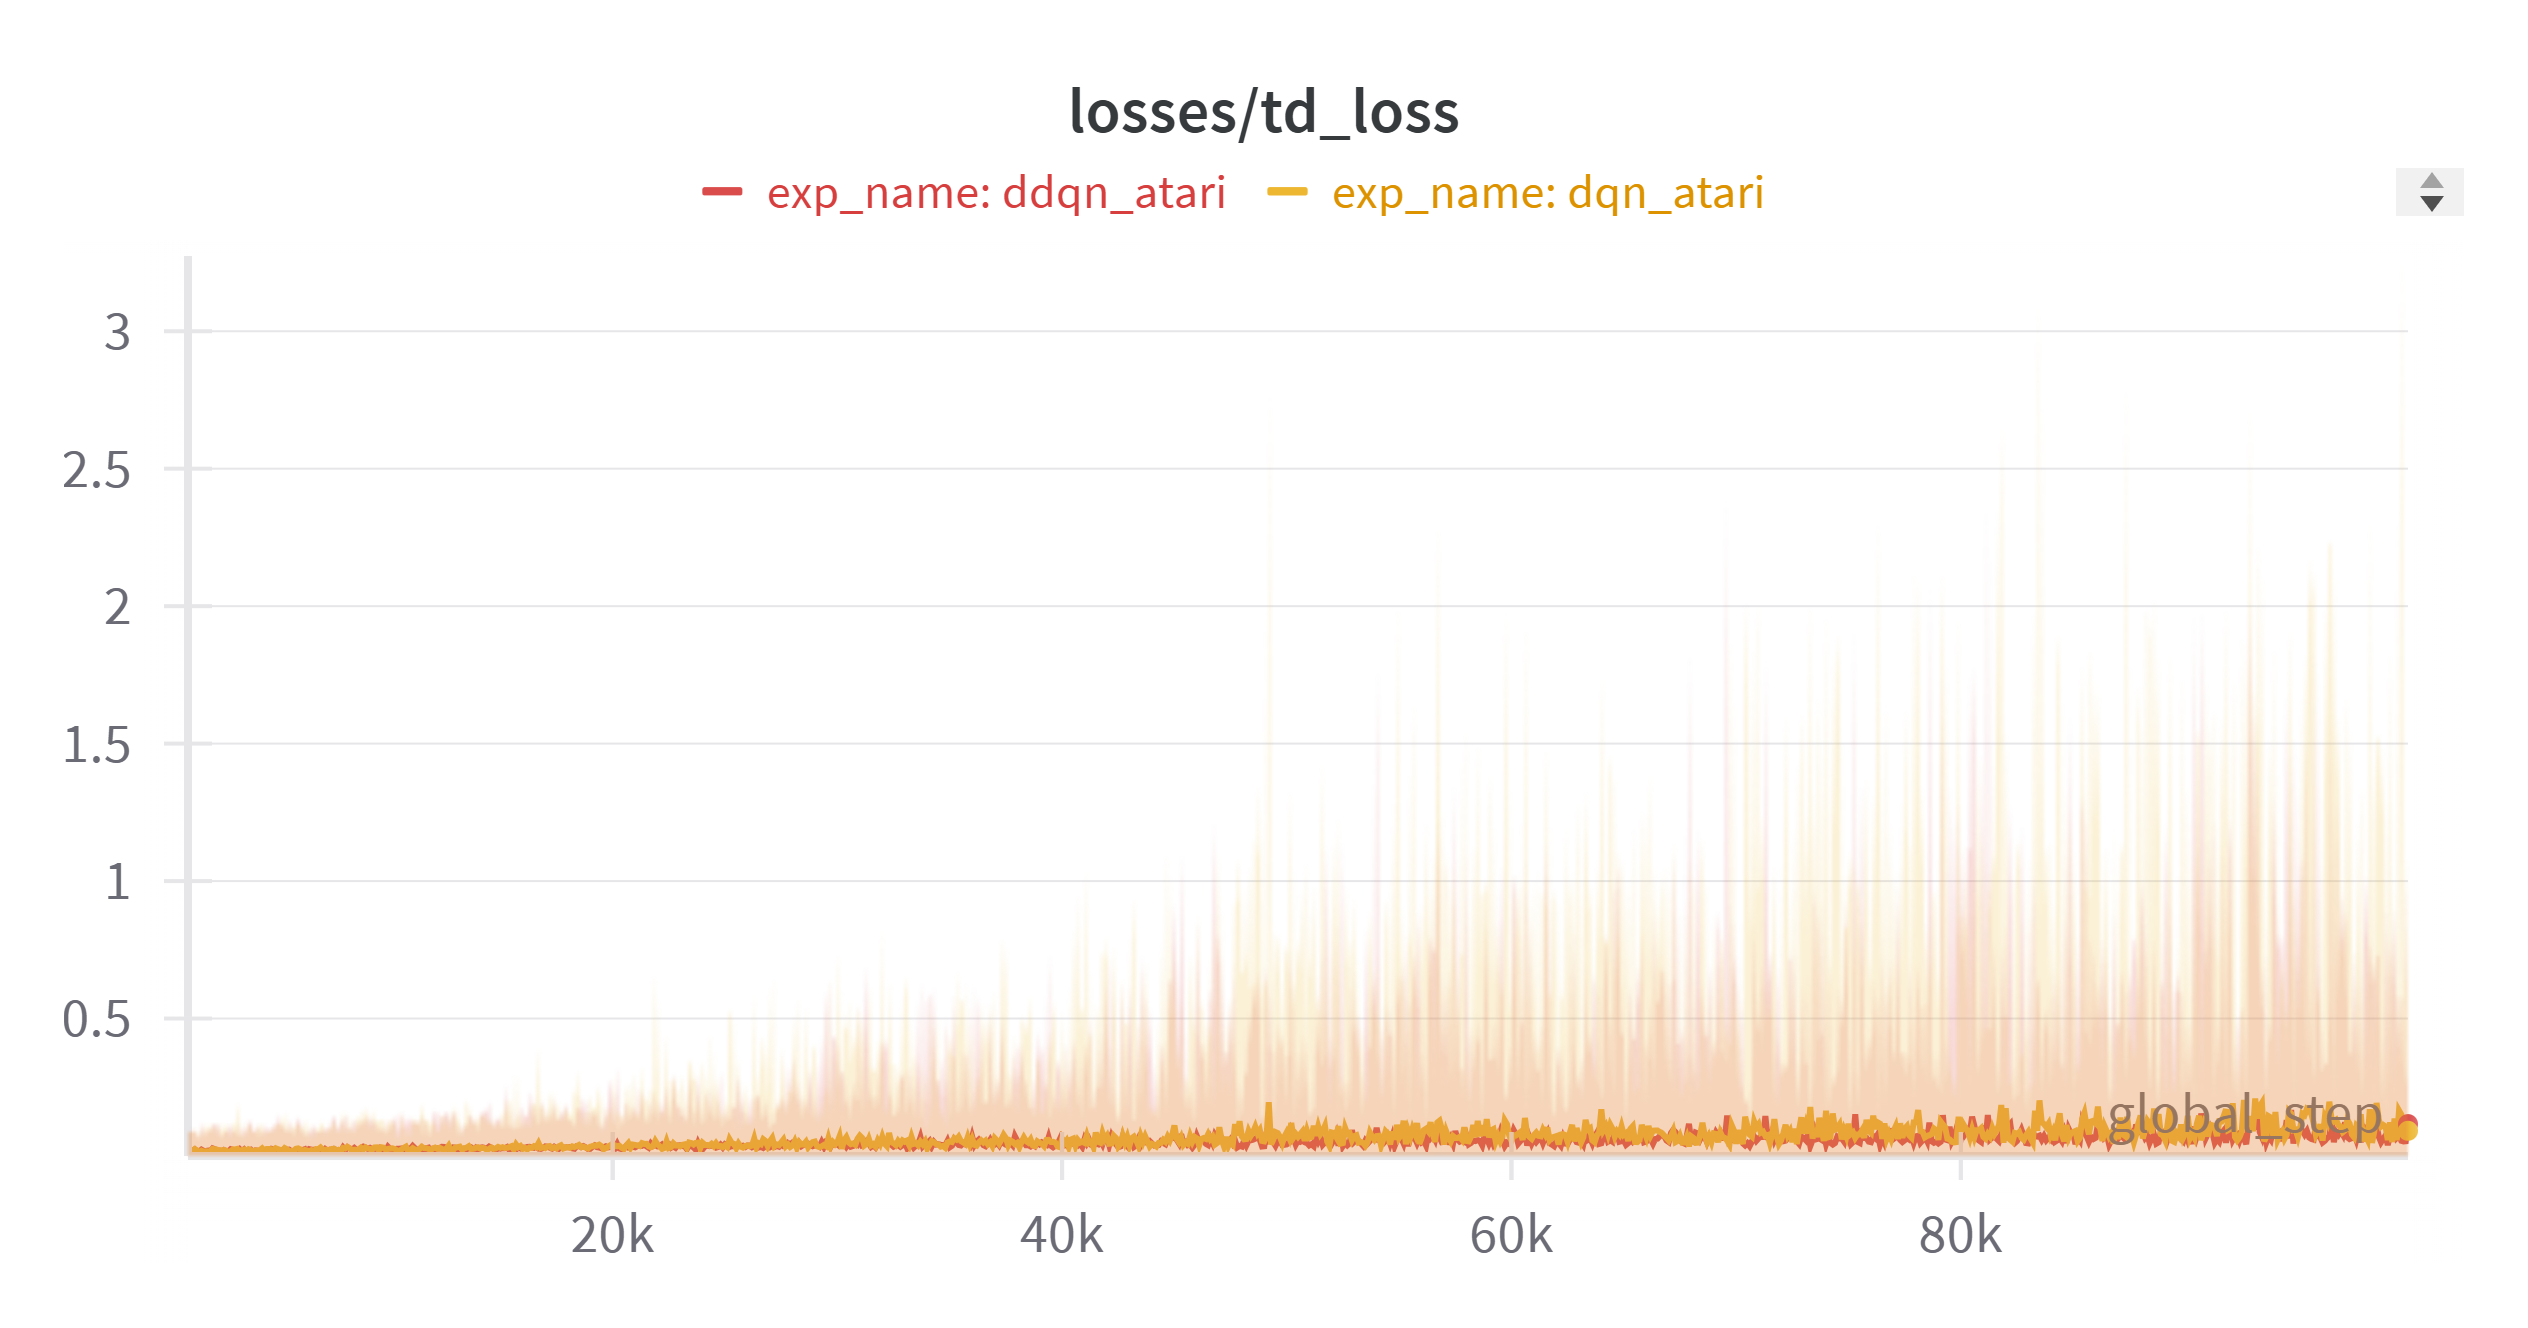
\includegraphics[width=0.6\textwidth]{figures/ddqn/comparison_losses_td_loss_dqn_ddqn.png}
	\caption{Comparison of TD loss for DQN (gold) vs.\ Double DQN (red). 
		Both remain near 0 for extended periods, though DQN shows slightly higher spikes.}
	\label{fig:dqn_vs_ddqn_td_loss}
\end{figure}


\begin{figure}
	\centering
	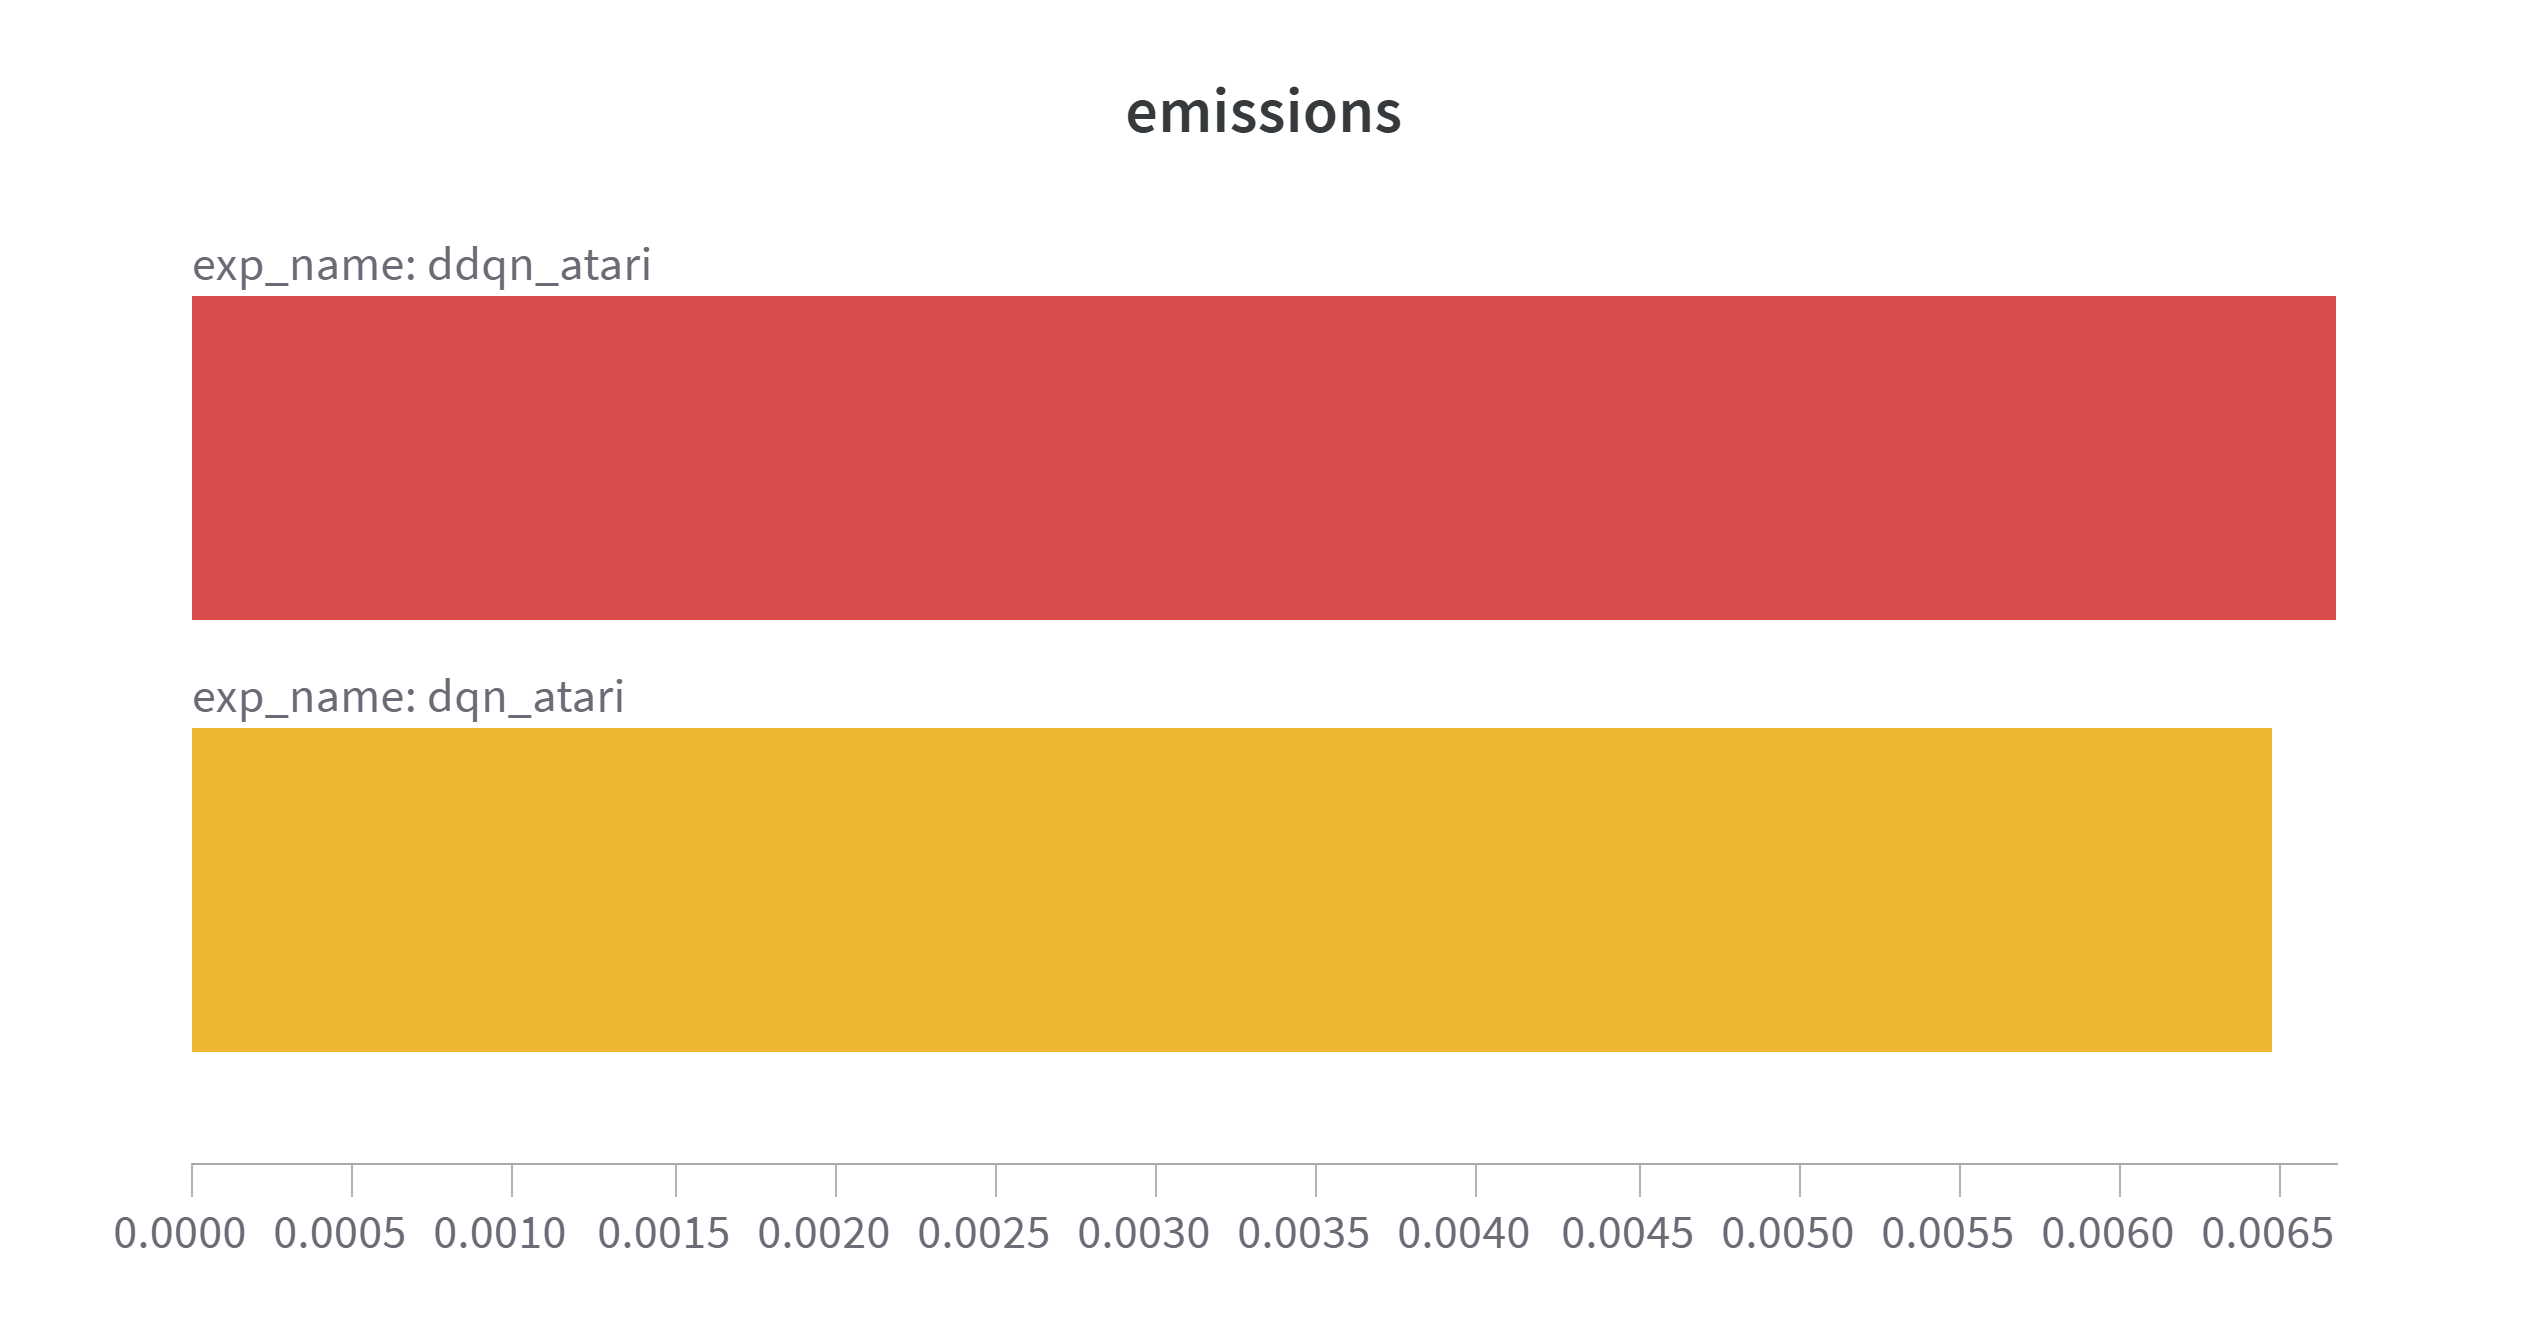
\includegraphics[width=0.6\textwidth]{figures/ddqn/emissions_dqn_ddqn.png}
	\caption{Mean emissions of DQN (gold) and Double DQN (red).}
	\label{fig:emissions_dqn_ddqn}
\end{figure}

Overall, Double DQN indeed moderates Q-value inflation compared to standard DQN, 
but under the 100k-step constraint, this reduction in overestimation does not strongly translate 
into consistently higher final returns.

\paragraph{Observations}
\begin{itemize}
	\item \textbf{Q-values and Losses:} Double DQN’s Q-values peak lower than DQN’s (about 2--3 vs.\ 4--5), aligning with the bias-reduction theory. TD losses remain small for both algorithms, with occasional spikes.
	\item \textbf{Performance:} The min--max normalized mean (0.374) is nearly the same as DQN’s (0.380), while human-normalized is actually lower (0.023 vs.\ 0.135) due to certain highly negative runs, especially in \emph{Boxing}.
	\item \textbf{Emissions:} Average $\sim0.00667$\,kg CO\textsubscript{2}-eq, slightly higher than DQN’s $0.00647$\,kg.
\end{itemize}

Hence, although Double DQN successfully limits Q-value overestimation, its advantage does not 
fully manifest in higher aggregate returns at 100k steps—indicating that more extensive training 
or additional refinements may be needed to reap its potential performance gains.


\subsubsection{Prioritized Experience Replay}
\label{subsubsec:per}

\paragraph{(Hyper)Parameters}

\begin{table}
	\caption{Key hyperparameters for Prioritized Experience Replay (PER). Only \texttt{env\_id} and \texttt{seed} vary across runs.}
	\label{tab:per_hyperparams}
	\centering
	\begin{tabular}{ll}
		\toprule
		\textbf{Parameter} & \textbf{Value} \\
		\midrule
		\texttt{exp\_name}                & per\_atari \\
		\texttt{seed}                     & 1..4 \\
		\texttt{torch\_deterministic}     & True \\
		\texttt{cuda}                     & True \\
		\texttt{track}                    & True \\
		\texttt{wandb\_project\_name}     & rlsb \\
		\texttt{capture\_video}           & False \\
		\texttt{save\_model}              & True \\
		\texttt{upload\_model}            & False \\
		\texttt{env\_id}                  & e.g.\ AmidarNoFrameskip-v4 \\
		\texttt{total\_timesteps}         & 100000 \\
		\texttt{learning\_rate}           & 0.0001 \\
		\texttt{num\_envs}                & 1 \\
		\texttt{buffer\_size}             & 10000 \\
		\texttt{gamma}                    & 0.99 \\
		\texttt{tau}                      & 1.0 \\
		\texttt{target\_network\_frequency} & 1000 \\
		\texttt{batch\_size}             & 32 \\
		\texttt{start\_e}, \texttt{end\_e} & 1.0 $\to$ 0.01 \\
		\texttt{exploration\_fraction}    & 0.1 \\
		\texttt{learning\_starts}         & 1000 \\
		\texttt{train\_frequency}         & 4 \\
		\bottomrule
	\end{tabular}
\end{table}

\paragraph{Hyperparameter Tuning}
We retained the same settings as baseline DQN (Section~\ref{subsubsec:dqn_baseline}) to highlight PER’s impact alone. Although \cite{schaul:prioritized} suggests lowering the learning rate by a factor of four, our tests at 100k steps showed $1\times10^{-4}$ worked better. Figure~\ref{fig:per_lr_comparison} compares these rates on \emph{Breakout}, indicating faster convergence at $1\times10^{-4}$.  

We also explored two implementations of the PER replay buffer—a \texttt{numpy}-based priority queue (for consistency) and a \texttt{torch}-based version. The \texttt{numpy} approach proved much slower, so we used the \texttt{torch} buffer in the final runs. Although the other DQN variants employ somewhat different replay optimizations (some from Stable Baselines), these differences did not appear to invalidate direct comparisons.

\begin{figure}
	\centering
	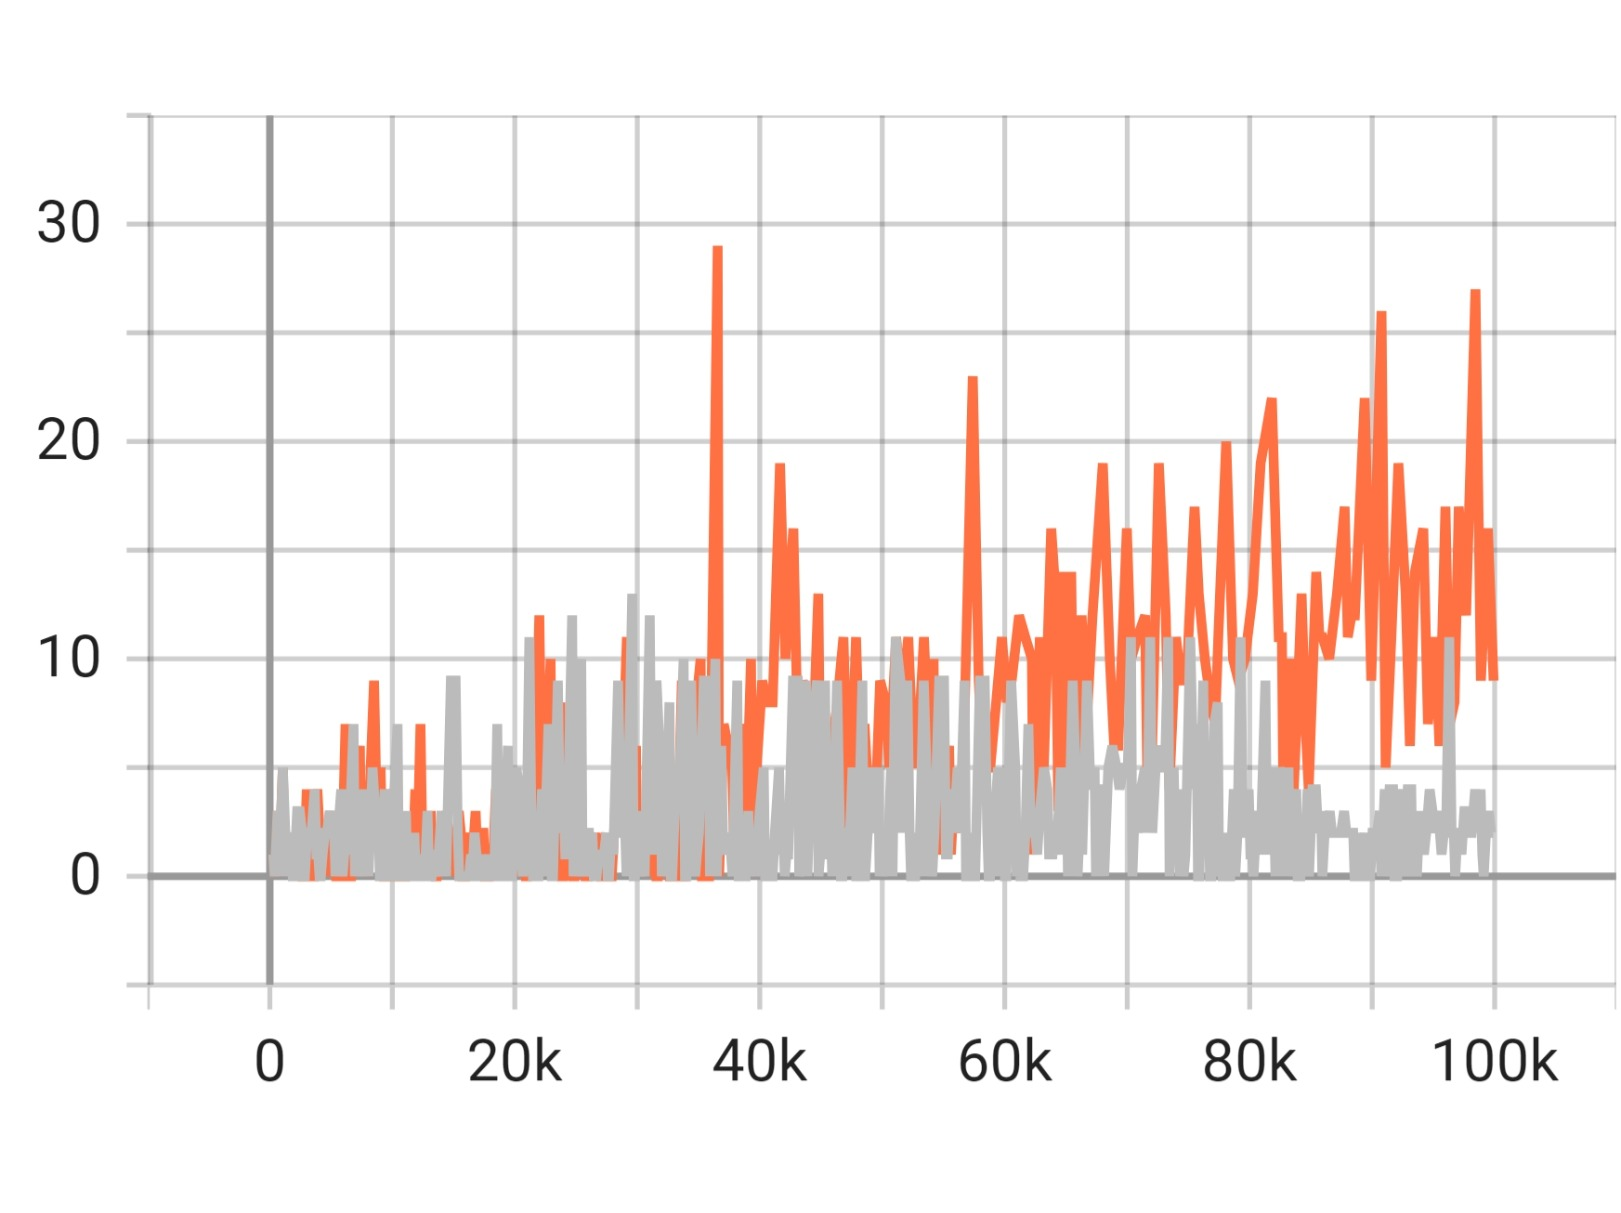
\includegraphics[width=0.55\textwidth]{figures/per/per_lr_charts_episodic_return.jpeg}
	\caption{Comparison of learning rates for PER on \emph{Breakout}. 
		Orange curve: $1\times10^{-4}$ (our final choice). 
		Gray curve: $\tfrac{1}{4}\times10^{-4}$ (as per \cite{schaul:prioritized}).}
	\label{fig:per_lr_comparison}
\end{figure}

\paragraph{Training Dynamics}
Figure~\ref{fig:per_training_metrics} aggregates four key metrics (episodic length, steps per second, Q-values, and TD loss) over 32 runs (eight games, four seeds each):

\begin{figure}
	\centering
	\subfloat[][Episodic length (\texttt{charts\_episodic\_length}). 
	The mean hovers around 3500--4000, and min--max runs from near 0 up to 8000.]{
		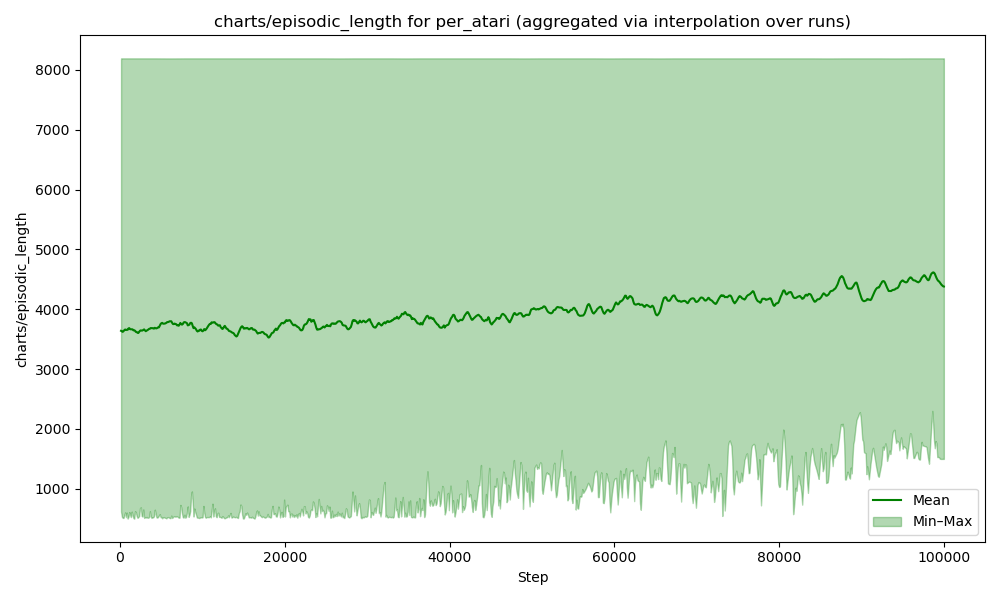
\includegraphics[width=.45\textwidth]{figures/per/charts_episodic_length_per_atari.png}
		\label{fig:per_episodic_length}
	}
	\quad
	\subfloat[][Steps per second (SPS). 
	The mean peaks above 170, then gradually declines to ~150--160.]{
		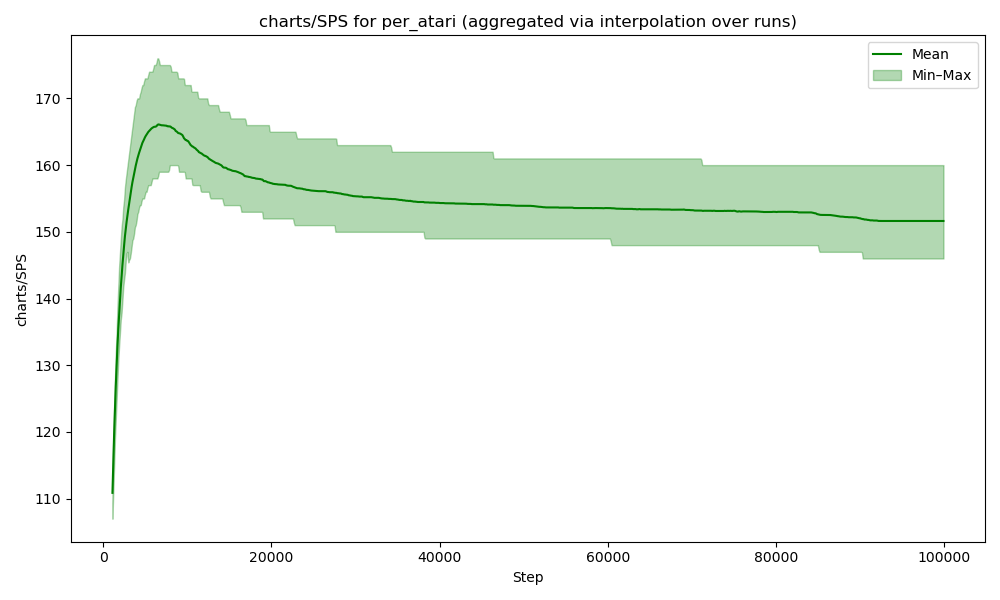
\includegraphics[width=.45\textwidth]{figures/per/charts_SPS_per_atari.png}
		\label{fig:per_sps}
	}
	\\[1em]
	\subfloat[][Q-values (\texttt{losses/q\_values}). 
	The mean eventually surpasses 4--5, with outliers above 14.]{
		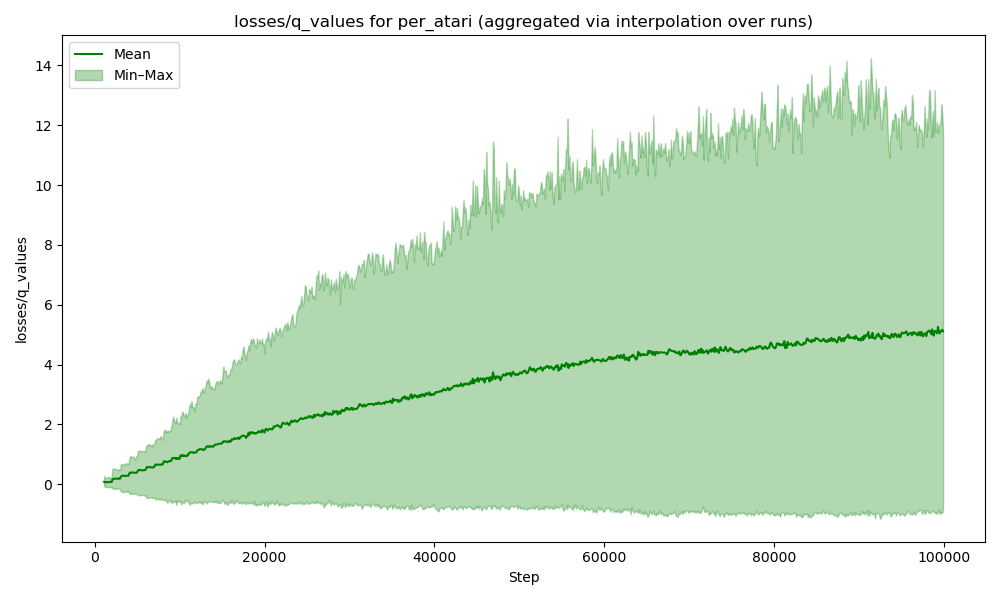
\includegraphics[width=.45\textwidth]{figures/per/losses_q_values_per_atari.png}
		\label{fig:per_q_values}
	}
	\quad
	\subfloat[][TD loss (\texttt{losses/td\_loss}). 
	Some runs spike above 3--4, showing instability in late training.]{
		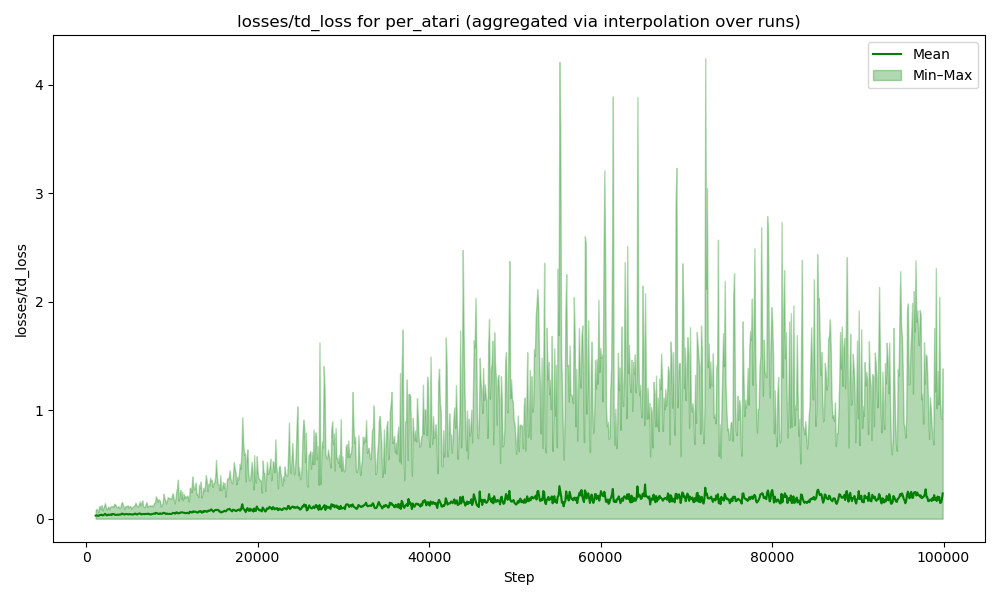
\includegraphics[width=.45\textwidth]{figures/per/losses_td_loss_per_atari.png}
		\label{fig:per_td_loss}
	}
	\caption{PER training metrics over 100k steps, interpolated across 32 runs.}
	\label{fig:per_training_metrics}
\end{figure}

PER shows Q-values approaching or exceeding those of baseline DQN (which typically topped at 4--5). The TD loss is small on average but spikes in certain runs, suggesting that prioritizing high-error samples can exacerbate updates in some episodes.

\paragraph{Episodic Return (Aggregated)}
Figures~\ref{fig:per_return_human} (human-normalized) and \ref{fig:per_return_minmax} (min--max) show PER’s aggregated episodic returns. The mean in human-normalized scale oscillates around zero, occasionally dipping below $-2$ or $-3$ in some seeds.

\begin{figure}
	\centering
	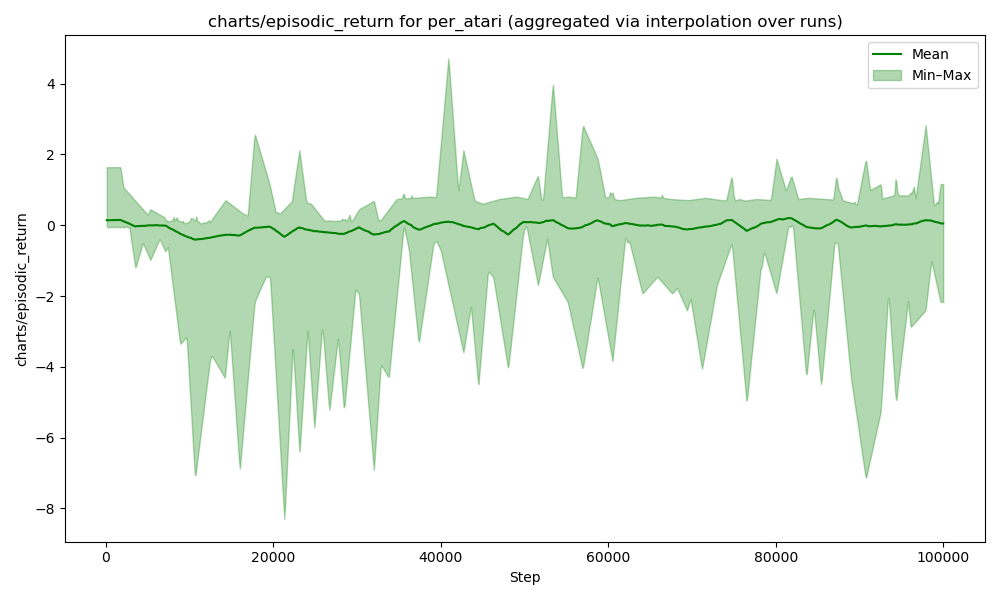
\includegraphics[width=0.6\textwidth]{figures/per/charts_episodic_return_human_per_atari.png}
	\caption{PER episodic return (human-normalized), aggregated over 32 runs. 
		Negative outliers appear for certain seeds/environments.}
	\label{fig:per_return_human}
\end{figure}

\begin{figure}
	\centering
	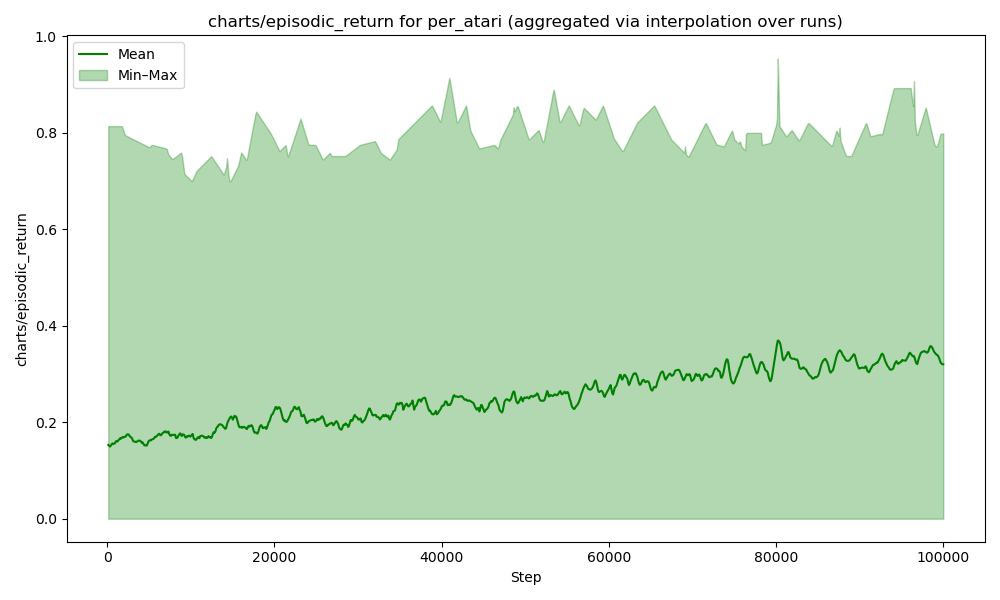
\includegraphics[width=0.6\textwidth]{figures/per/charts_episodic_return_minmax_per_atari.png}
	\caption{PER episodic return (min--max normalized), aggregated over 32 runs.}
	\label{fig:per_return_minmax}
\end{figure}

\paragraph{Per-Game Returns}
Figures~\ref{fig:per_return_pergame_human} and \ref{fig:per_return_pergame_minmax} break down the performance by each Atari game (human vs. min--max normalization). We see, for instance, \emph{Freeway} (orange line in min--max) steadily climbing to around 0.7--0.8, while \emph{Alien} can drop below $-3$ in human scale. 

\begin{figure}
	\centering
	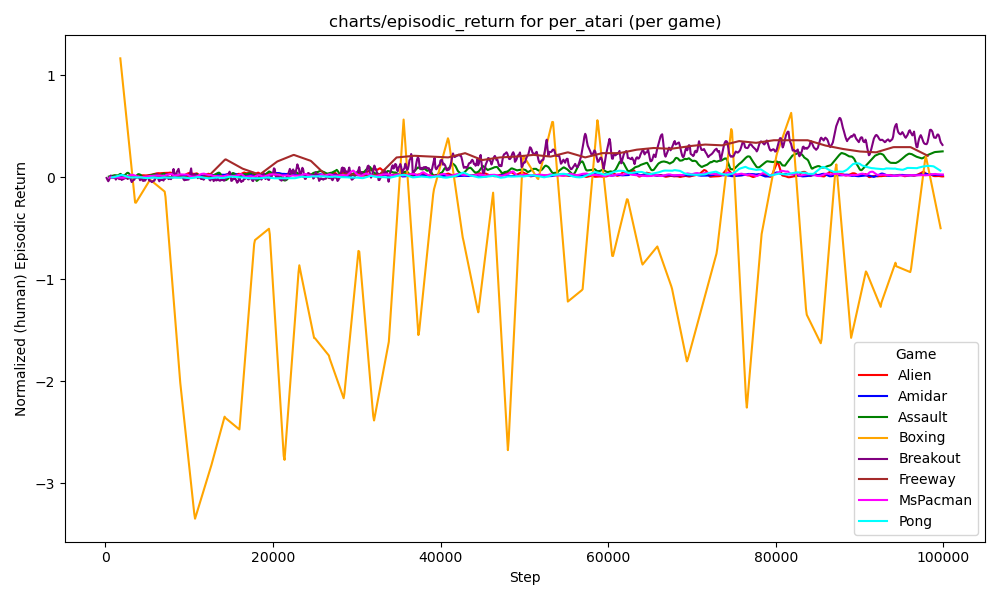
\includegraphics[width=0.6\textwidth]{figures/per/charts_episodic_return_per_game_human_per_atari.png}
	\caption{PER returns per game (human-normalized). 
		\emph{Alien} (orange) exhibits deep negative dips, 
		while \emph{Freeway}, \emph{Assault}, and \emph{Breakout} stay near or above zero.}
	\label{fig:per_return_pergame_human}
\end{figure}

\begin{figure}
	\centering
	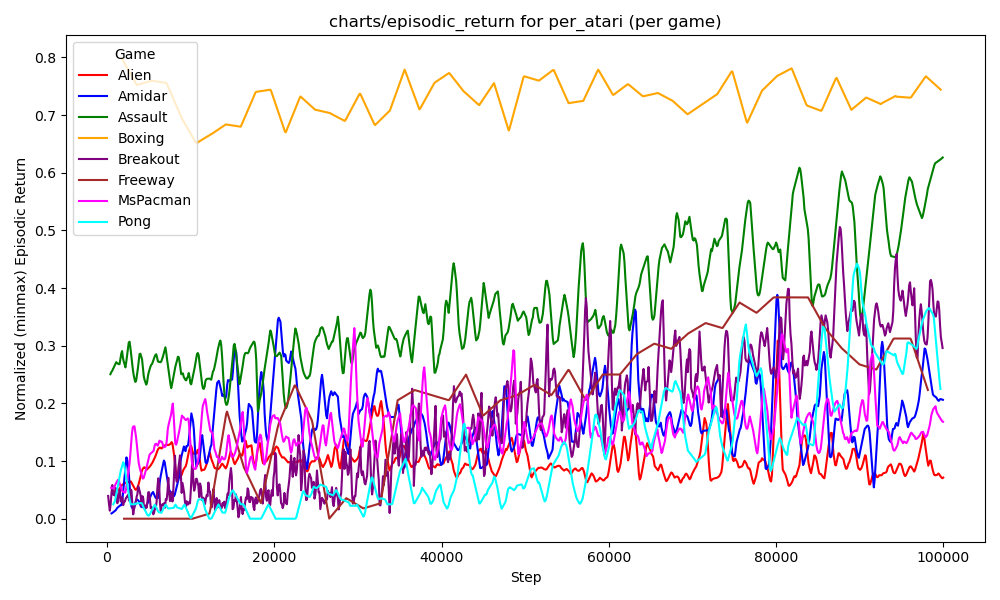
\includegraphics[width=0.6\textwidth]{figures/per/charts_episodic_return_per_game_minmax_per_atari.png}
	\caption{PER returns per game (min--max normalized). 
		\emph{Freeway} (gold line) and \emph{Assault} (green) reach 0.7--0.8 near 100k steps.}
	\label{fig:per_return_pergame_minmax}
\end{figure}

\paragraph{Emissions.}

\begin{table}
	\caption{Carbon emissions (kg\,CO\textsubscript{2}eq) for PER across 32 runs.}
	\label{tab:per_emissions}
	\centering
	\makebox[\textwidth]{%
	\begin{tabularx}{1.1\textwidth}{lXXXXXXXX}
		\toprule
		\textbf{Algorithm} & \textbf{mean} & \textbf{std} & \textbf{median} & \textbf{q25} & \textbf{q75} & \textbf{min} & \textbf{max} & \textbf{iqmean} \\
		\midrule
		PER & 0.007254 & 0.000263 & 0.007146 & 0.007074 & 0.007354 & 0.006935 & 0.007819 & 0.007157 \\
		\bottomrule
	\end{tabularx}
	}
\end{table}

Figure~\ref{fig:per_vs_dqn_emissions} shows a barplot comparing PER’s mean emissions (\(\approx 0.00725\,\mathrm{kg}\)) to DQN’s (\(\approx0.00647\,\mathrm{kg}\)). The overhead of prioritized sampling may partly account for this higher footprint.

\begin{figure}
	\centering
	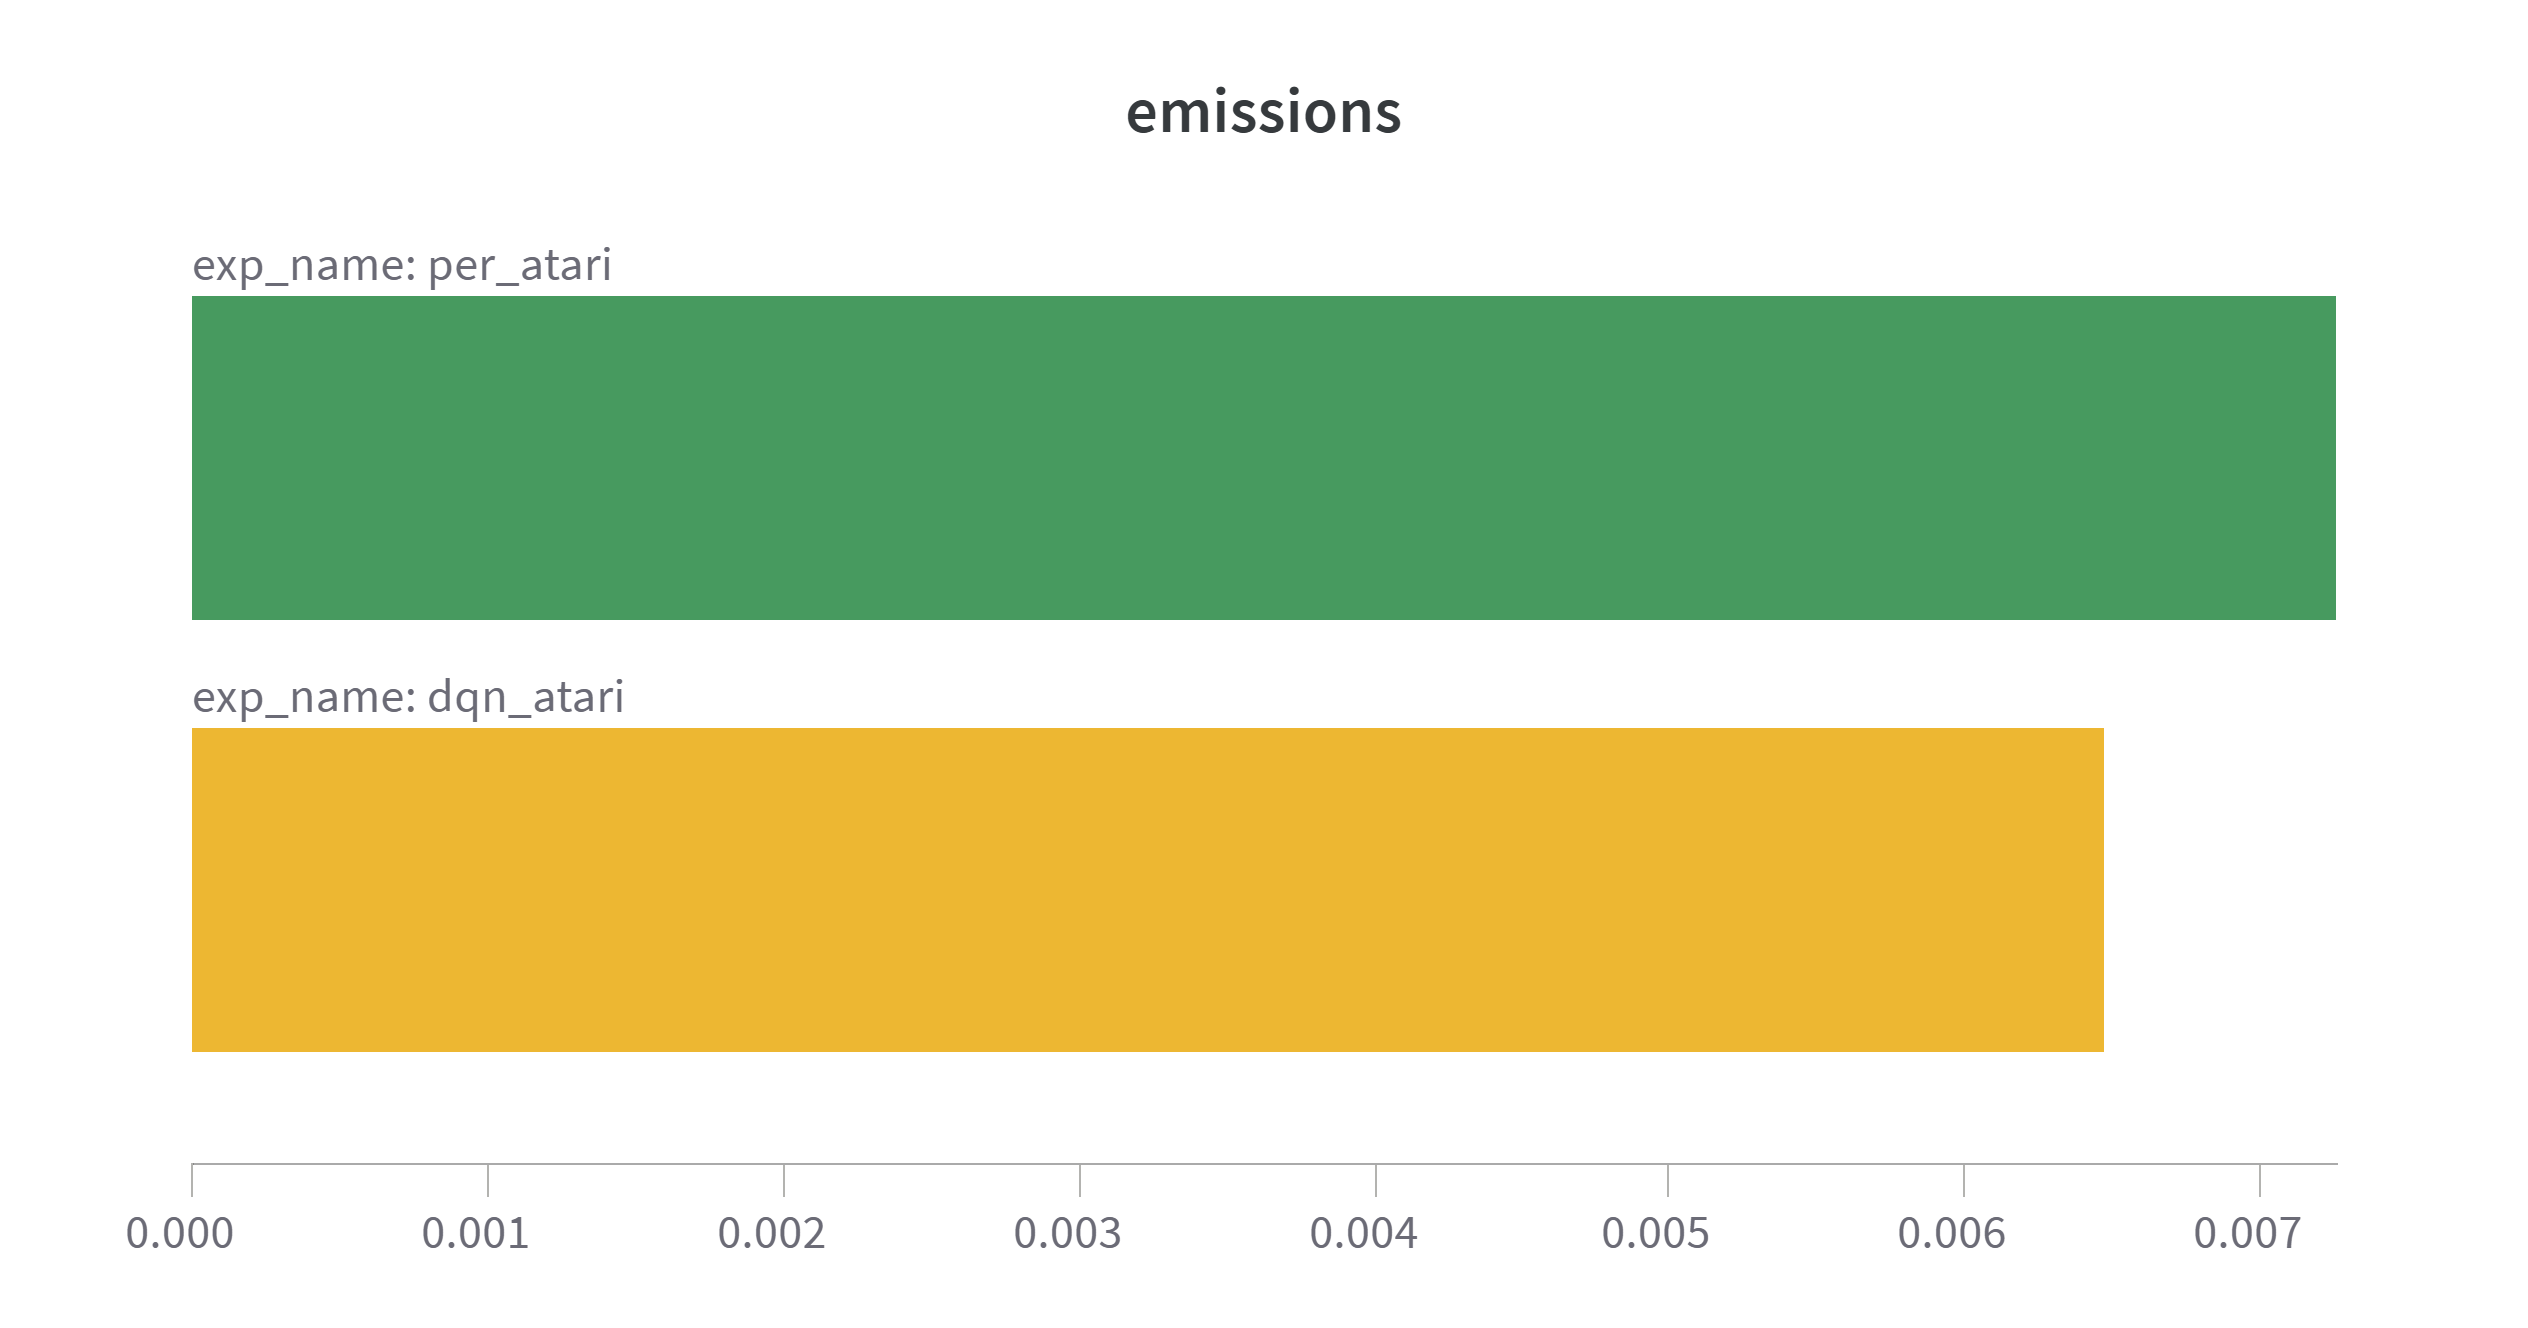
\includegraphics[width=0.55\textwidth]{figures/per/emissions_dqn_per.png}
	\caption{Mean emissions comparison: PER (green) at $\sim0.00725$\,kg vs.\ DQN (gold) at $\sim0.00647$\,kg.}
	\label{fig:per_vs_dqn_emissions}
\end{figure}

\begin{table}
	\caption{Overall final evaluation (10 episodes each) for PER across 32 runs.}
	\label{tab:per_eval_overall}
	\centering
	\begin{tabular}{lcccccccc}
		\toprule
		\textbf{Normalization} & \textbf{mean} & \textbf{std} & \textbf{median} & 
		\textbf{q25} & \textbf{q75} & \textbf{min} & \textbf{max} & \textbf{iqmean} \\
		\midrule
		\textbf{Human}   & 0.0607 & 1.0170 & 0.0539 & 0.0175 & 0.2541 & -10.2619 & 6.8809 & 0.0813 \\
		\textbf{Min--Max}& 0.3533 & 0.2695 & 0.2583 & 0.1499 & 0.6265 & 0.0 & 0.9845 & 0.3087 \\
		\bottomrule
	\end{tabular}
\end{table}

\begin{table}
	\caption{Per-game final evaluation for PER (human- vs.\ min--max normalized). Each row aggregates 10 episodes $\times$ 4 seeds per environment.}
	\label{tab:per_eval_gamewise}
	\centering
	\begin{tabular}{llcccc}
		\toprule
		\textbf{Game} & \textbf{Norm} & \textbf{mean} & \textbf{std} & \textbf{min} & \textbf{max}\\
		\midrule
		Alien     & Human    & 0.0246 & 0.0315 & -0.0147 & 0.0996 \\
		& Min--Max & 0.0978 & 0.0523 & 0.0325  & 0.2225 \\
		\cmidrule{1-6}
		Amidar    & Human    & 0.0263 & 0.0220 & -0.0029 & 0.0809 \\
		& Min--Max & 0.2288 & 0.1693 & 0.0046  & 0.6498 \\
		\cmidrule{1-6}
		Assault   & Human    & 0.2135 & 0.0974 & 0.0232  & 0.3860 \\
		& Min--Max & 0.5648 & 0.1480 & 0.2757  & 0.8270 \\
		\cmidrule{1-6}
		Boxing    & Human    & -0.6667 & 2.7351 & -10.2619 & 6.8809 \\
		& Min--Max & 0.7388  & 0.0890 & 0.4264    & 0.9845 \\
		\cmidrule{1-6}
		Breakout  & Human    & 0.3854 & 0.2204 & 0.00997 & 0.9070 \\
		& Min--Max & 0.3500 & 0.1746 & 0.0526  & 0.7632 \\
		\cmidrule{1-6}
		Freeway   & Human    & 0.4071 & 0.3381 & 0.0     & 0.8446 \\
		& Min--Max & 0.4304 & 0.3574 & 0.0     & 0.8929 \\
		\cmidrule{1-6}
		MsPacman  & Human    & 0.0338 & 0.0111 & 0.0119 & 0.0515 \\
		& Min--Max & 0.2008 & 0.0446 & 0.1126 & 0.2723 \\
		\cmidrule{1-6}
		Pong      & Human    & 0.0617 & 0.0682 & -0.01 & 0.2233 \\
		& Min--Max & 0.2150 & 0.2045 & 0.0   & 0.7000 \\
		\bottomrule
	\end{tabular}
\end{table}

\paragraph{Comparison with Baseline DQN.}
By final evaluation, PER’s overall human-norm mean (0.0607) is lower than DQN’s (0.135), and its min--max mean (0.353) lags behind DQN’s 0.380.  
Figure~\ref{fig:per_vs_dqn_emissions} further shows PER’s emissions exceed DQN’s by $\sim0.0008$\,kg CO\textsubscript{2}-eq on average—likely due to the overhead from prioritized sampling and somewhat longer average episodes.

\paragraph{Observations.}
\begin{itemize}
	\item \textbf{Implementation Details:} 
	We used a \texttt{torch}-based PER buffer to avoid severe slowdowns in the \texttt{numpy} version.
	\item \textbf{Learning Rate:} 
	$\tfrac{1}{4}\times10^{-4}$, as suggested in \cite{schaul:prioritized}, underperformed at 100k steps 
	compared to $1\times10^{-4}$ (Figure~\ref{fig:per_lr_comparison}).
	\item \textbf{Performance:} 
	PER did not consistently outperform baseline DQN within 100k steps: 
	human-norm mean is 0.0607 vs.\ DQN’s 0.135. 
	\item \textbf{Emissions:} 
	PER's overhead leads to slightly higher energy usage (0.00725\,kg CO\textsubscript{2}-eq) than DQN’s 0.00647\,kg.
\end{itemize}

In summary, while prioritizing high-error samples can yield benefits in longer training runs, 
our 100k-step Atari benchmark does not showcase a strong advantage. 
Further hyperparameter tuning or more extended runs might better reveal PER’s strengths.


\subsubsection{Dueling DQN}
\label{subsubsec:dueling_dqn}

\paragraph{(Hyper)Parameters}

\begin{table}
	\caption{Key hyperparameters for Dueling DQN. Only \texttt{env\_id} and \texttt{seed} vary across runs.}
	\label{tab:dueling_dqn_hyperparams}
	\centering
	\begin{tabular}{ll}
		\toprule
		\textbf{Parameter} & \textbf{Value} \\
		\midrule
		\texttt{exp\_name}                & dueling\_dqn\_atari \\
		\texttt{seed}                     & 1..4 \\
		\texttt{torch\_deterministic}     & True \\
		\texttt{cuda}                     & True \\
		\texttt{track}                    & True \\
		\texttt{wandb\_project\_name}     & rlsb \\
		\texttt{capture\_video}           & False \\
		\texttt{save\_model}              & True \\
		\texttt{upload\_model}            & False \\
		\texttt{env\_id}                  & e.g.\ AlienNoFrameskip-v4 \\
		\texttt{total\_timesteps}         & 100000 \\
		\texttt{learning\_rate}           & 0.0001 \\
		\texttt{num\_envs}                & 1 \\
		\texttt{buffer\_size}             & 10000 \\
		\texttt{gamma}                    & 0.99 \\
		\texttt{tau}                      & 1.0 \\
		\texttt{target\_network\_frequency} & 1000 \\
		\texttt{batch\_size}             & 32 \\
		\texttt{start\_e}, \texttt{end\_e} & 1.0 $\to$ 0.01 \\
		\texttt{exploration\_fraction}    & 0.1 \\
		\texttt{learning\_starts}         & 1000 \\
		\texttt{train\_frequency}         & 4 \\
		\bottomrule
	\end{tabular}
\end{table}

\paragraph{Innovation: Dueling Architecture}
The \emph{Dueling DQN}~\cite{wang:dueling} architecture modifies the final layers of a Q-network
to separate the estimation of state-value $V(s)$ from advantage $A(s,a)$.
These two “heads” are combined to yield
\[
Q(s,a) = V(s) + A(s,a) \;-\; \frac{1}{|\mathcal{A}|}\sum_{a'} A(s,a'),
\]
which aims to stabilize learning in states where the choice of action is less critical.

\noindent
\textbf{Network Size Note}:
Because the dueling architecture introduces separate streams for $V$ and $A$, the model ends up
with slightly more parameters. We considered reducing the size of the shared layer to keep the
overall parameter count equal to the baseline, but the difference was only about 512 neurons,
so we retained the original layer size for consistency with the other DQN variants.
We also tested whether gradient clipping (as mentioned in some references) would improve
stability, but found no clear benefit here.
Finally, we did not combine dueling with Double DQN or PER, as our goal is to isolate the contribution
of this single tweak in terms of performance and emissions.

\paragraph{Training Dynamics}

\begin{figure}
	\centering
	\subfloat[][Episodic length. 
	The mean hovers around 3500--4000 steps, with min--max from near 0 up to 8000.]{
		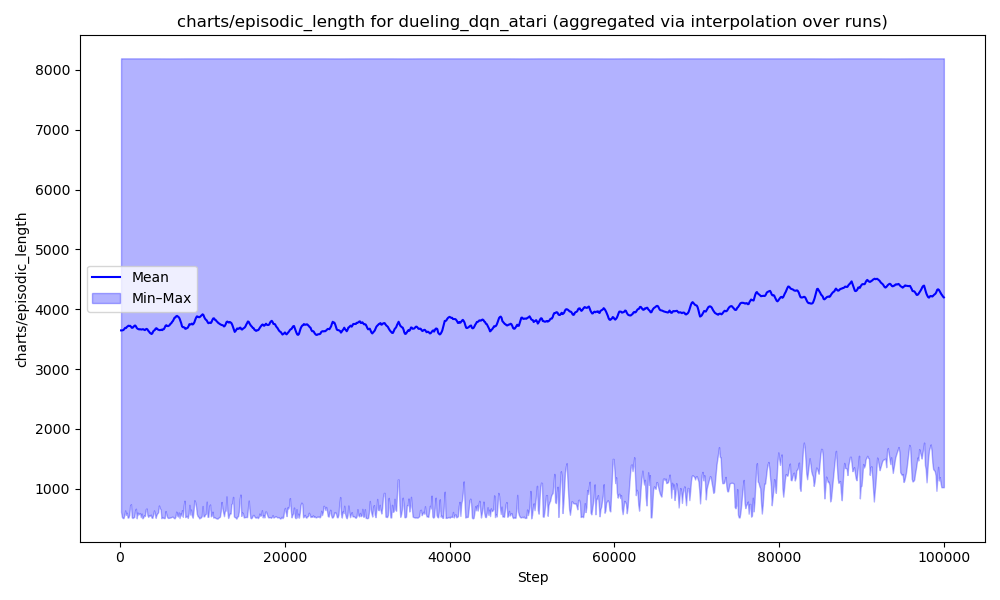
\includegraphics[width=.45\textwidth]{figures/dueling_dqn/charts_episodic_length_dueling_dqn_atari.png}
		\label{fig:dueling_episodic_length}
	}
	\quad
	\subfloat[][Steps per second (SPS). 
	After an initial ramp-up near 170, it stabilizes around 155--160.]{
		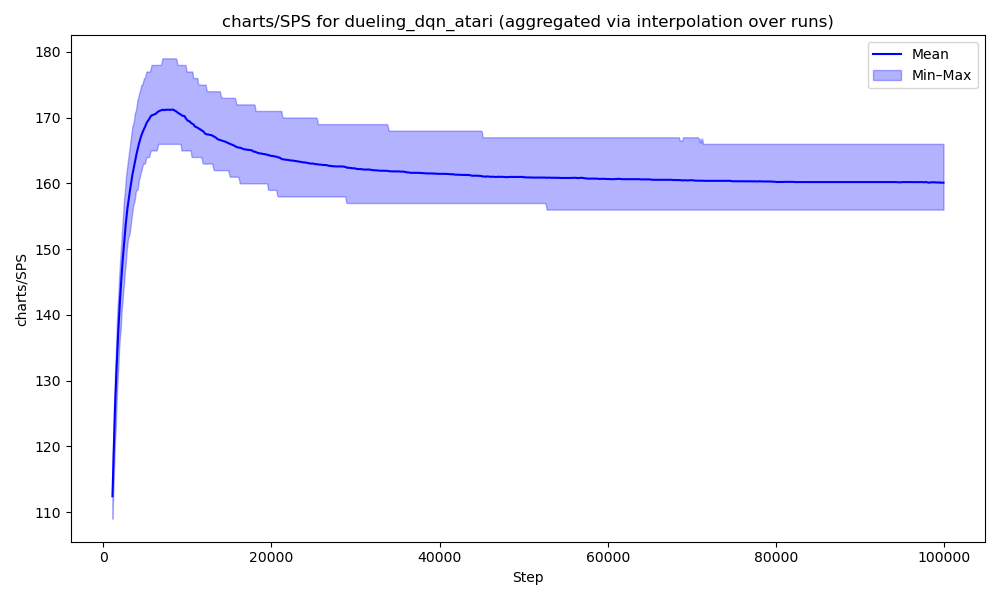
\includegraphics[width=.45\textwidth]{figures/dueling_dqn/charts_SPS_dueling_dqn_atari.png}
		\label{fig:dueling_sps}
	}
	\\[1em]
	\subfloat[][Q-values (\texttt{losses/q\_values}). 
	The mean grows beyond 4--5, with outliers near 8--10.]{
		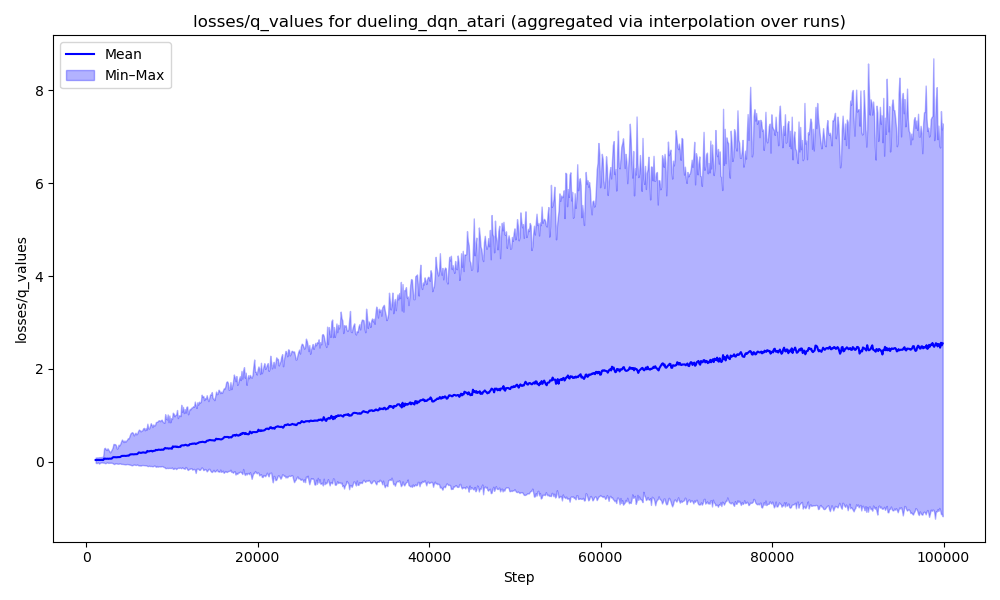
\includegraphics[width=.45\textwidth]{figures/dueling_dqn/losses_q_values_dueling_dqn_atari.png}
		\label{fig:dueling_q_values}
	}
	\quad
	\subfloat[][TD loss (\texttt{losses/td\_loss}). 
	Some runs spike above 1.5--2.0, showing moderate variability late in training.]{
		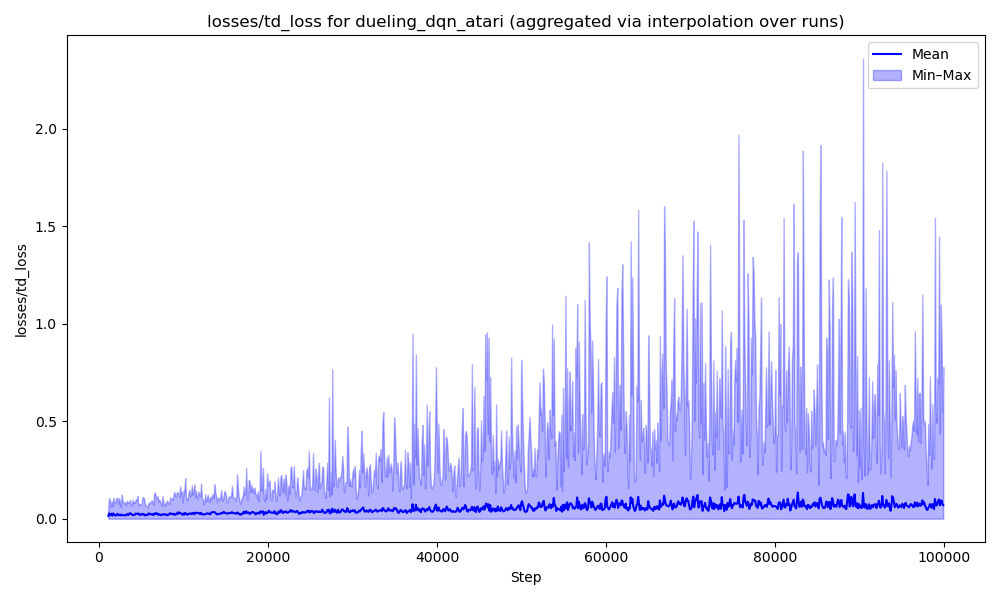
\includegraphics[width=.45\textwidth]{figures/dueling_dqn/losses_td_loss_dueling_dqn_atari.png}
		\label{fig:dueling_td_loss}
	}
	\caption{Dueling DQN training metrics over 100k steps, aggregated over 32 runs.}
	\label{fig:dueling_training_metrics}
\end{figure}

\paragraph{Episodic Return (Aggregated)}

\begin{figure}
	\centering
	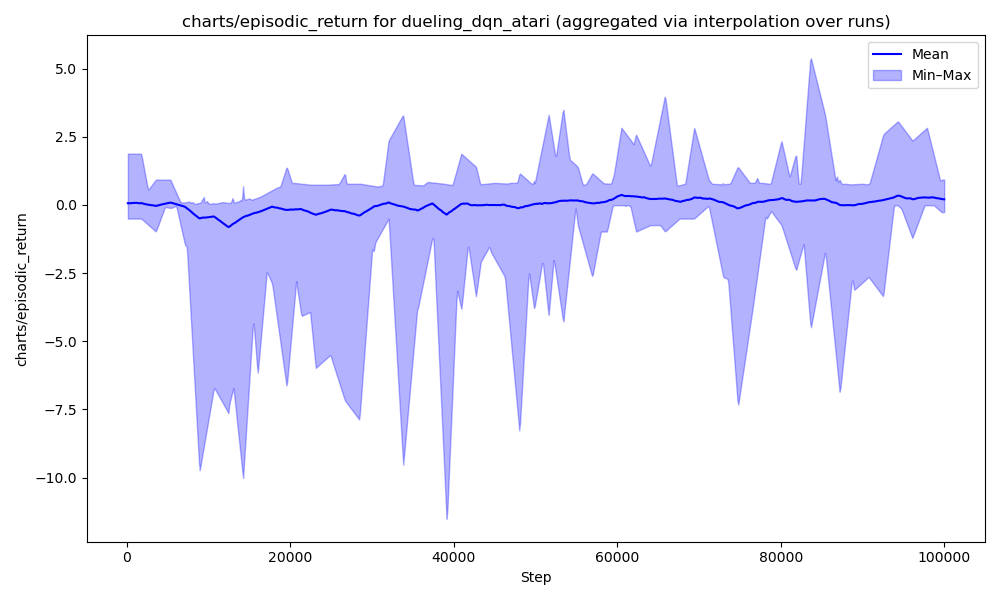
\includegraphics[width=0.6\textwidth]{figures/dueling_dqn/charts_episodic_return_human_dueling_dqn_atari.png}
	\caption{Dueling DQN episodic return (human-normalized) over 100k steps. 
		Variance is significant, with some dips below -8.}
	\label{fig:dueling_return_human}
\end{figure}

\begin{figure}
	\centering
	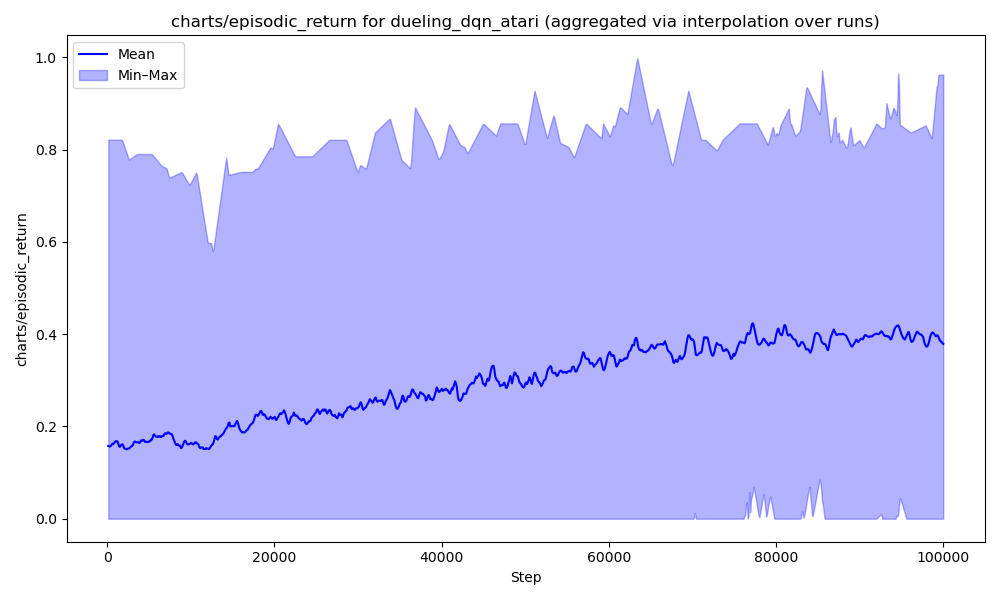
\includegraphics[width=0.6\textwidth]{figures/dueling_dqn/charts_episodic_return_minmax_dueling_dqn_atari.png}
	\caption{Dueling DQN episodic return (min--max normalized) aggregated over 32 runs.}
	\label{fig:dueling_return_minmax}
\end{figure}

\paragraph{Per-Game Returns}

\begin{figure}
	\centering
	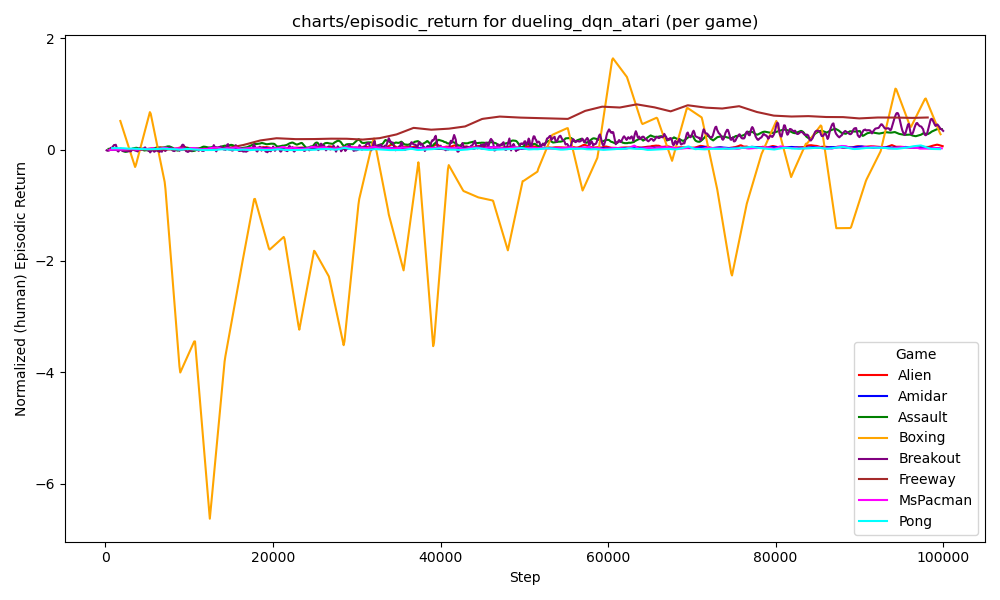
\includegraphics[width=0.6\textwidth]{figures/dueling_dqn/charts_episodic_return_per_game_human_dueling_dqn_atari.png}
	\caption{Dueling DQN returns per game (human-normalized). 
		\emph{Boxing} (orange) experiences deep negative dips, while \emph{Freeway} and \emph{Assault} can reach higher normalized scores.}
	\label{fig:dueling_return_pergame_human}
\end{figure}

\begin{figure}
	\centering
	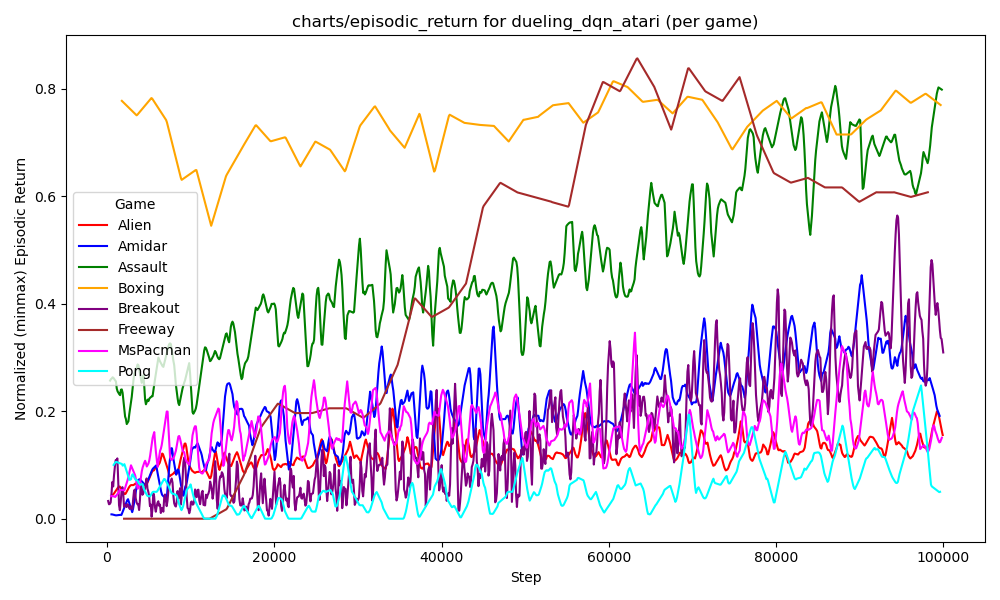
\includegraphics[width=0.6\textwidth]{figures/dueling_dqn/charts_episodic_return_per_game_minmax_dueling_dqn_atari.png}
	\caption{Dueling DQN returns per game (min--max normalized). 
		\emph{Freeway} (gold) and \emph{Assault} (green) often exceed 0.7.}
	\label{fig:dueling_return_pergame_minmax}
\end{figure}

\paragraph{Emissions}

\begin{table}
	\caption{Carbon emissions (kg\,CO\textsubscript{2}eq) for Dueling DQN across 32 runs.}
	\label{tab:dueling_dqn_emissions}
	\centering
	\begin{tabular}{lcccccccc}
		\toprule
		\textbf{Algorithm} & \textbf{mean} & \textbf{std} & \textbf{median} & 
		\textbf{q25} & \textbf{q75} & \textbf{min} & \textbf{max} & \textbf{iqmean} \\
		\midrule
		Dueling DQN & 0.006893 & 0.0002901 & 0.006742 & 0.006672 & 0.007002 & 0.006617 & 0.007478 & 0.006779 \\
		\bottomrule
	\end{tabular}
\end{table}

\begin{figure}
	\centering
	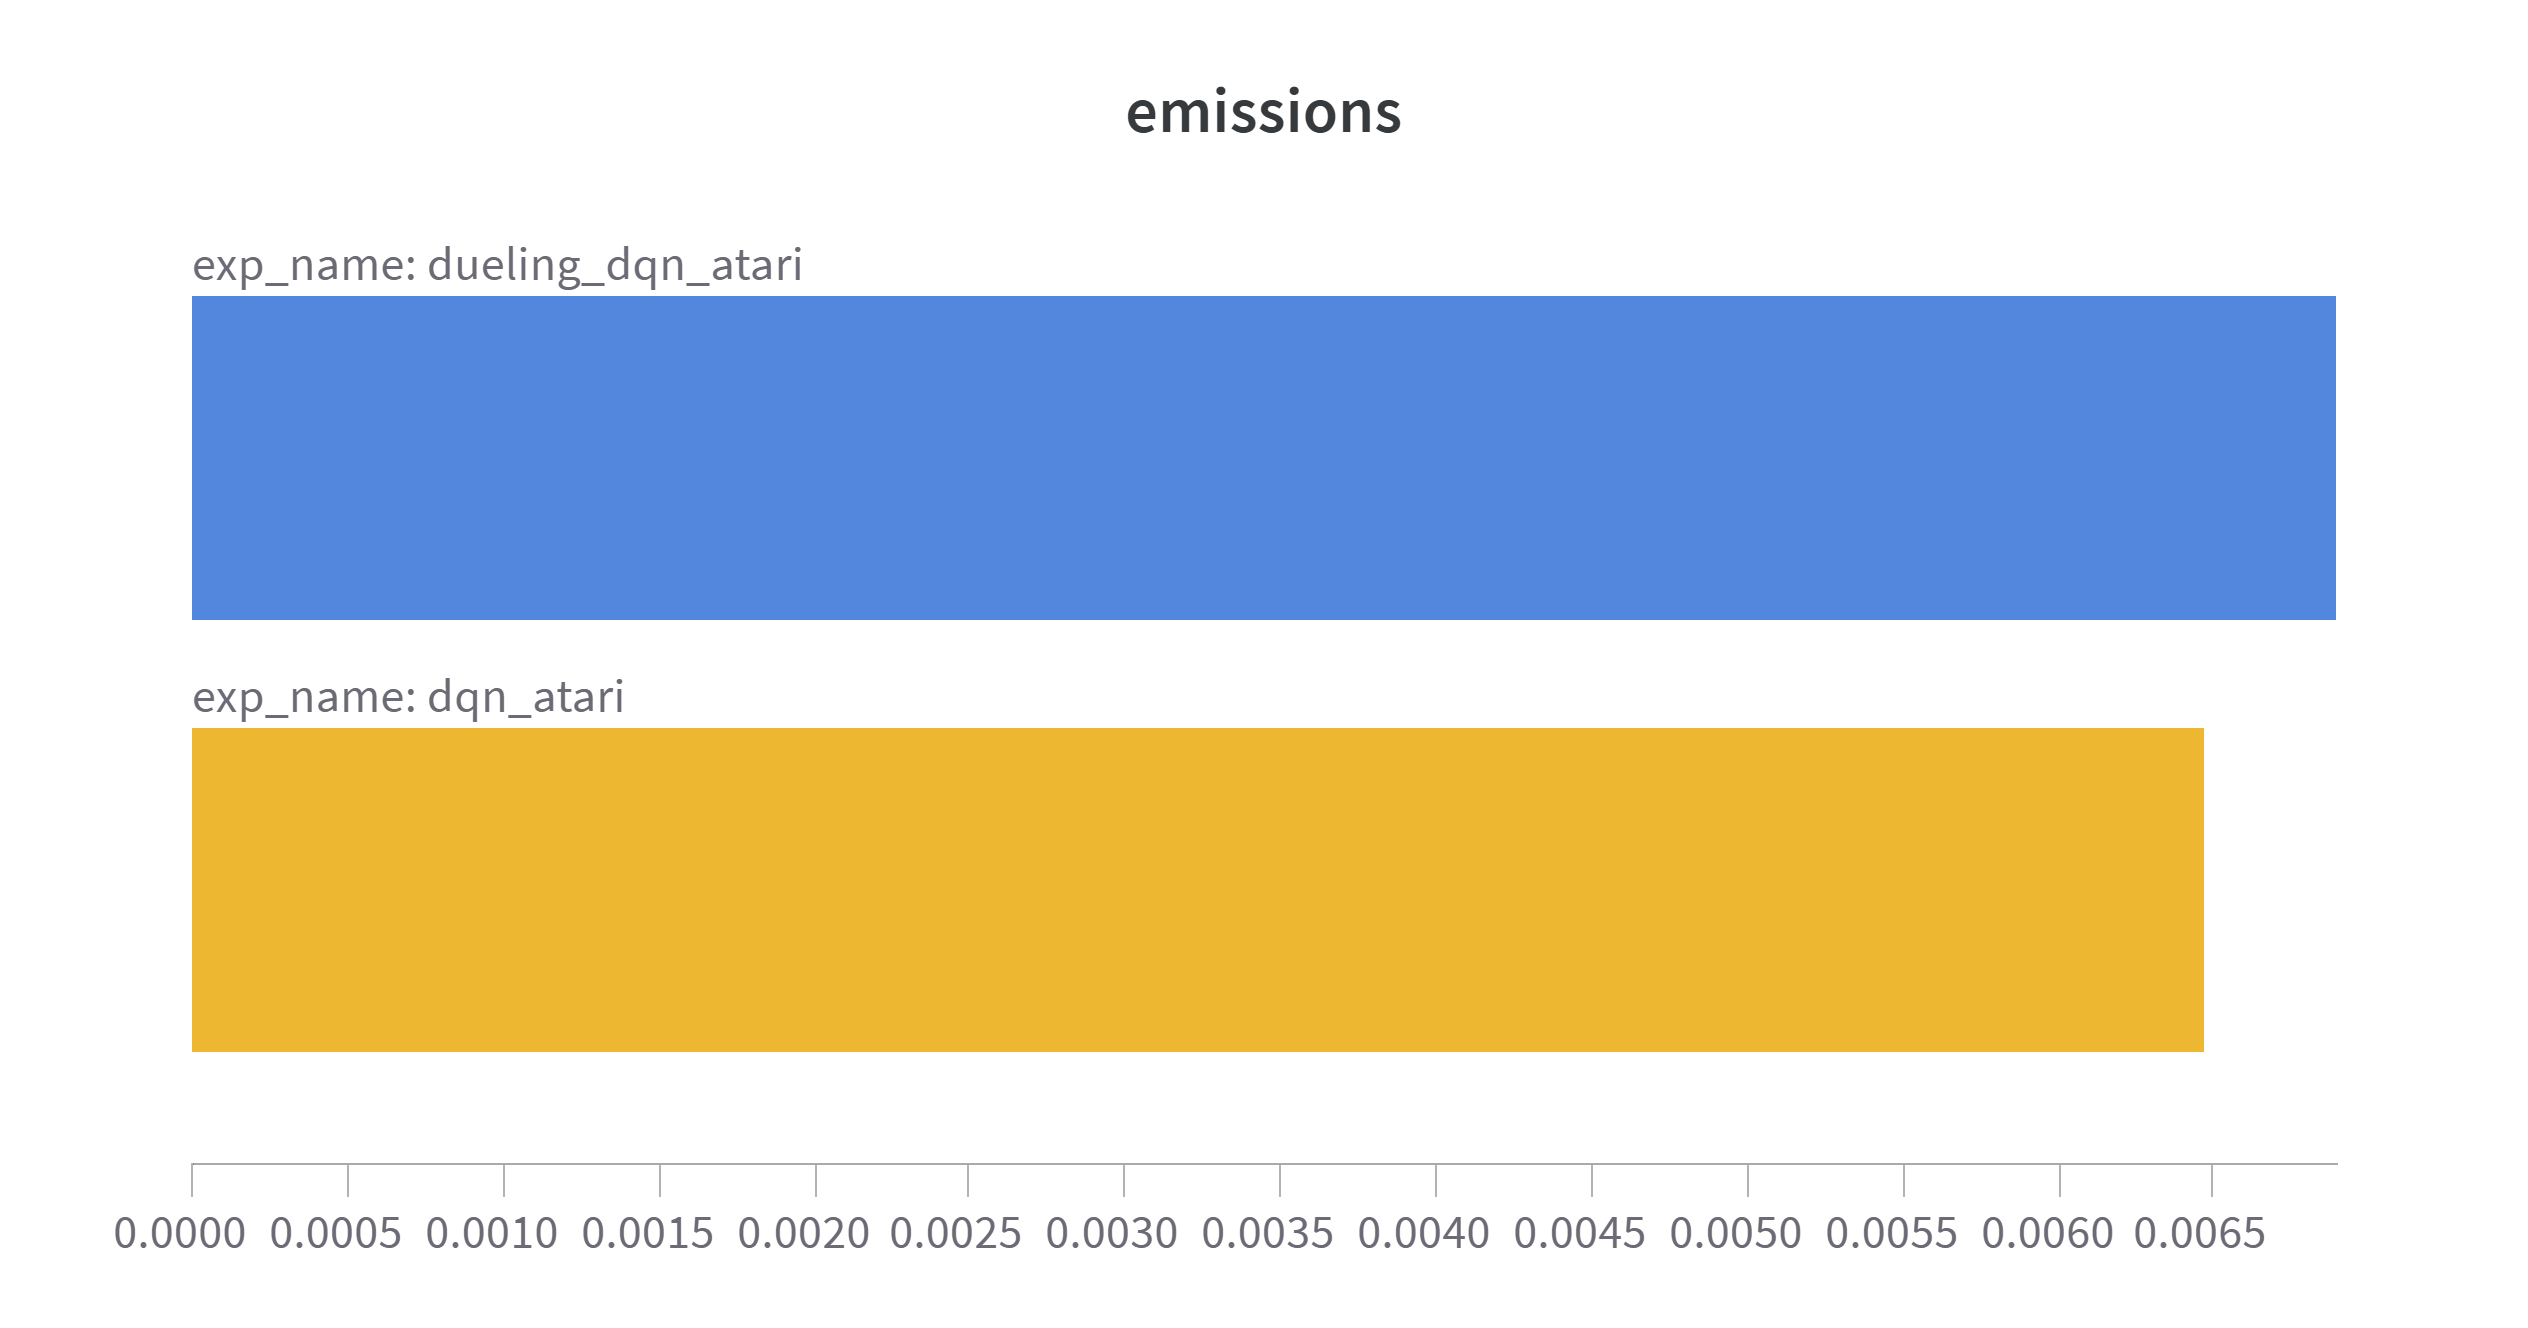
\includegraphics[width=0.55\textwidth]{figures/dueling_dqn/emissions_dqn_dueling.png}
	\caption{Mean emissions comparison: Dueling DQN (blue) at $\sim0.00689$\,kg vs.\ DQN (gold) at $\sim0.00647$\,kg.}
	\label{fig:dueling_emissions_barplot}
\end{figure}

\paragraph{Evaluation Results}

\begin{table}
	\caption{Overall final evaluation (10 episodes each) for Dueling DQN across 32 runs.}
	\label{tab:dueling_dqn_eval_overall}
	\centering
	\begin{tabular}{lcccccccc}
		\toprule
		\textbf{Normalization} & \textbf{mean} & \textbf{std} & \textbf{median} & 
		\textbf{q25} & \textbf{q75} & \textbf{min} & \textbf{max} & \textbf{iqmean} \\
		\midrule
		\textbf{Human}   & 0.1860 & 0.5258 & 0.0402 & 0.0148 & 0.3530 & -1.9286 & 3.5476 & 0.1020 \\
		\textbf{Min--Max}& 0.3849 & 0.3056 & 0.2632 & 0.1100 & 0.7448 & 0.0 & 0.9523 & 0.3454 \\
		\bottomrule
	\end{tabular}
\end{table}

\begin{table}
	\caption{Per-game final evaluation for Dueling DQN (human- vs.\ min--max normalized).}
	\label{tab:dueling_dqn_eval_gamewise}
	\centering
	\begin{tabular}{llcccc}
		\toprule
		\textbf{Game} & \textbf{Norm} & \textbf{mean} & \textbf{std} & \textbf{min} & \textbf{max}\\
		\midrule
		Alien     & Human    & 0.0398 & 0.0346 & -0.0072 & 0.1493 \\
		& Min--Max & 0.1231 & 0.0574 & 0.0450  & 0.3050 \\
		\cmidrule{1-6}
		Amidar    & Human    & 0.0372 & 0.0193 & 0.0235 & 0.0935 \\
		& Min--Max & 0.3127 & 0.1482 & 0.2074 & 0.7465 \\
		\cmidrule{1-6}
		Assault   & Human    & 0.3200 & 0.0985 & 0.1057 & 0.4684 \\
		& Min--Max & 0.7266 & 0.1498 & 0.4010 & 0.9523 \\
		\cmidrule{1-6}
		Boxing    & Human    & 0.1190 & 1.3282 & -1.9286 & 3.5476 \\
		& Min--Max & 0.7643 & 0.0432 & 0.6977  & 0.8760 \\
		\cmidrule{1-6}
		Breakout  & Human    & 0.4020 & 0.2904 & -0.0565 & 1.0066 \\
		& Min--Max & 0.3632 & 0.2300 & 0.0     & 0.8421 \\
		\cmidrule{1-6}
		Freeway   & Human    & 0.5372 & 0.3162 & 0.0     & 0.7770 \\
		& Min--Max & 0.5679 & 0.3342 & 0.0     & 0.8214 \\
		\cmidrule{1-6}
		MsPacman  & Human    & 0.0265 & 0.0204 & 0.00018 & 0.0736 \\
		& Min--Max & 0.1713 & 0.0823 & 0.0654  & 0.3613 \\
		\cmidrule{1-6}
		Pong      & Human    & 0.0067 & 0.0185 & -0.01 & 0.0567 \\
		& Min--Max & 0.0500 & 0.0555 & 0.0   & 0.2 \\
		\bottomrule
	\end{tabular}
\end{table}

\paragraph{Comparison with Baseline DQN}
In final evaluation, Dueling DQN’s \emph{human}-norm mean is 0.1860 vs.\ DQN’s 0.1353, 
and the \emph{min--max} mean is 0.3849 vs.\ DQN’s 0.3802—so we see a small positive difference on average.
However, \emph{Boxing} outliers (some runs exceed 3.5, others dip below $-1.9$) inflate the variance.
Meanwhile, emissions at $\sim0.00689$\,kg CO\textsubscript{2}-eq are higher than DQN’s $\sim0.00647$ but remain
lower than some other variants (e.g.\ PER at 0.00725).

\paragraph{Observations}
\begin{itemize}
	\item \textbf{Architecture Impact:}
	The \emph{dueling} approach separates state-value and advantage,
	intending to stabilize updates in states where action choices matter less.
	\item \textbf{Network Size:}
	We kept the same shared layer size as DQN, adding only a modest number of extra parameters.
	\item \textbf{Performance:}
	The final mean in human normalization (0.1860) is higher than baseline DQN’s 0.1353,
	though min--max (0.3849 vs.\ 0.3802) is only slightly larger.
	\item \textbf{Emissions:}
	Dueling DQN uses $\sim0.00689$\,kg CO\textsubscript{2}-eq,
	more than DQN’s 0.00647 but less than PER’s 0.00725.
\end{itemize}


\subsubsection{Categorical DQN (C51)}
\label{subsubsec:c51}

\paragraph{(Hyper)Parameters}

\begin{table}
	\caption{Key hyperparameters for the C51 algorithm. Only \texttt{env\_id} and \texttt{seed} vary across runs.}
	\label{tab:c51_hyperparams}
	\centering
	\begin{tabular}{ll}
		\toprule
		\textbf{Parameter} & \textbf{Value} \\
		\midrule
		\texttt{exp\_name}                & c51\_atari \\
		\texttt{seed}                     & 1..4 \\
		\texttt{torch\_deterministic}     & True \\
		\texttt{cuda}                     & True \\
		\texttt{track}                    & True \\
		\texttt{wandb\_project\_name}     & rlsb \\
		\texttt{capture\_video}           & False \\
		\texttt{save\_model}              & True \\
		\texttt{upload\_model}            & False \\
		\texttt{env\_id}                  & e.g.\ AlienNoFrameskip-v4 \\
		\texttt{total\_timesteps}         & 100000 \\
		\texttt{learning\_rate}           & 0.00025 \\
		\texttt{num\_envs}                & 1 \\
		\texttt{n\_atoms}                 & 51 \\
		\texttt{v\_min}                   & -10 \\
		\texttt{v\_max}                   & 10 \\
		\texttt{buffer\_size}             & 10000 \\
		\texttt{gamma}                    & 0.99 \\
		\texttt{target\_network\_frequency} & 1000 \\
		\texttt{batch\_size}             & 32 \\
		\texttt{start\_e}, \texttt{end\_e} & 1.0 $\to$ 0.01 \\
		\texttt{exploration\_fraction}    & 0.1 \\
		\texttt{learning\_starts}         & 1000 \\
		\texttt{train\_frequency}         & 4 \\
		\bottomrule
	\end{tabular}
\end{table}

\paragraph{Innovation: Distributional RL}
Categorical DQN (\textbf{C51})~\cite{bellemare:distributional} models $Q(s,a)$ 
as a discrete probability distribution over possible returns, using $\texttt{n\_atoms}$ support points 
that span the interval $[v_{\mathrm{min}},\,v_{\mathrm{max}}]$. 
By capturing more than a single expected value, C51 can potentially improve learning stability 
and performance, especially in risk- or variance-sensitive tasks.

\paragraph{Hyperparameter Tuning}
We adopted CleanRL’s \texttt{c51\_atari} configuration with 51 atoms, $v_{\min}=-10$, $v_{\max}=10$, 
and a learning rate of $2.5\times10^{-4}$. While we tested alternative rates, 
this default proved effective over only 100k steps.  

We also experimented with \texttt{target\_network\_frequency} values of 1k, 5k, and 10k 
to see if less frequent updates might reduce overhead. 
Ultimately, 1k provided a good balance of stable returns and moderate emissions, 
aligning with other DQN-based variants.

\paragraph{Training Dynamics}

\begin{figure}
	\centering
	\subfloat[][Episodic length (\texttt{charts\_episodic\_length}). 
	The mean is \(\sim 3500\)--\(4000\), while min--max occasionally spikes above 8000 or even 17500 in some runs.]{
		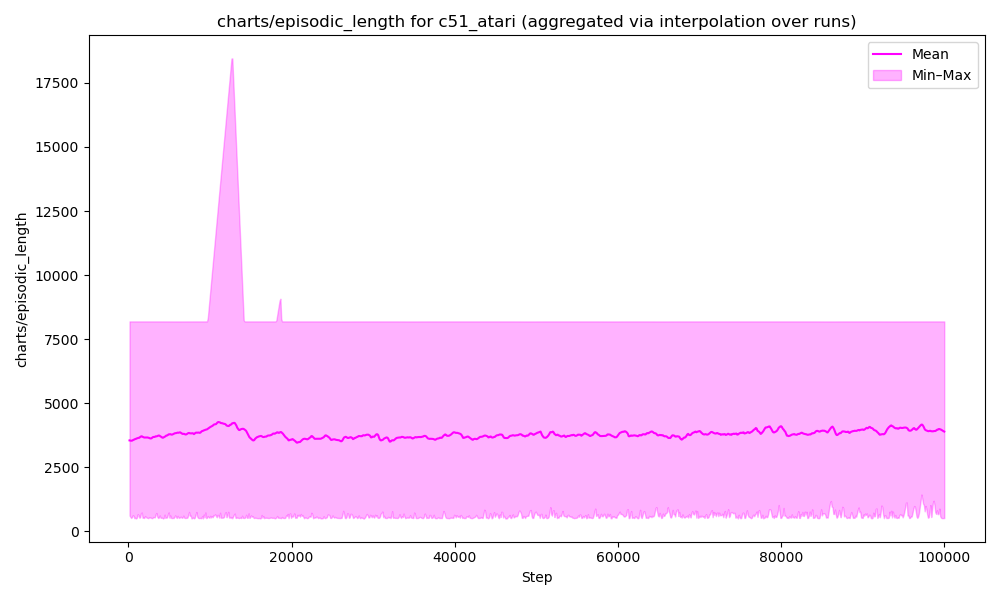
\includegraphics[width=.45\textwidth]{figures/c51/charts_episodic_length_c51_atari.png}
		\label{fig:c51_episodic_length}
	}
	\quad
	\subfloat[][Steps per second (SPS).
	Mean peaks around 160--170, then slowly converges near 140--150.]{
		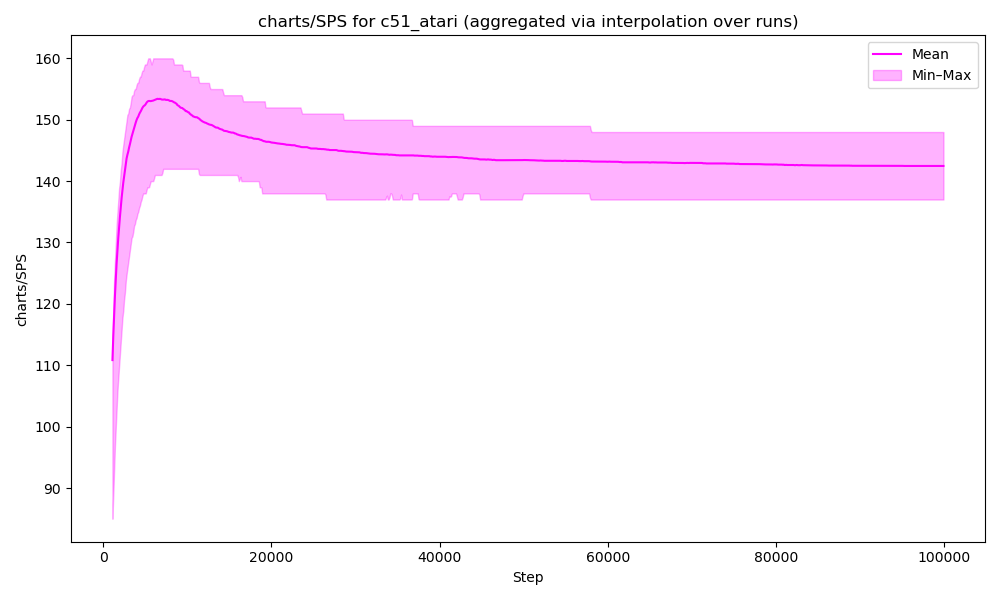
\includegraphics[width=.45\textwidth]{figures/c51/charts_SPS_c51_atari.png}
		\label{fig:c51_sps}
	}
	\\[1em]
	\subfloat[][Overall loss (\texttt{losses/loss}). 
	The mean steadily declines from about 4.0 toward near 2.0 by the end of training.]{
		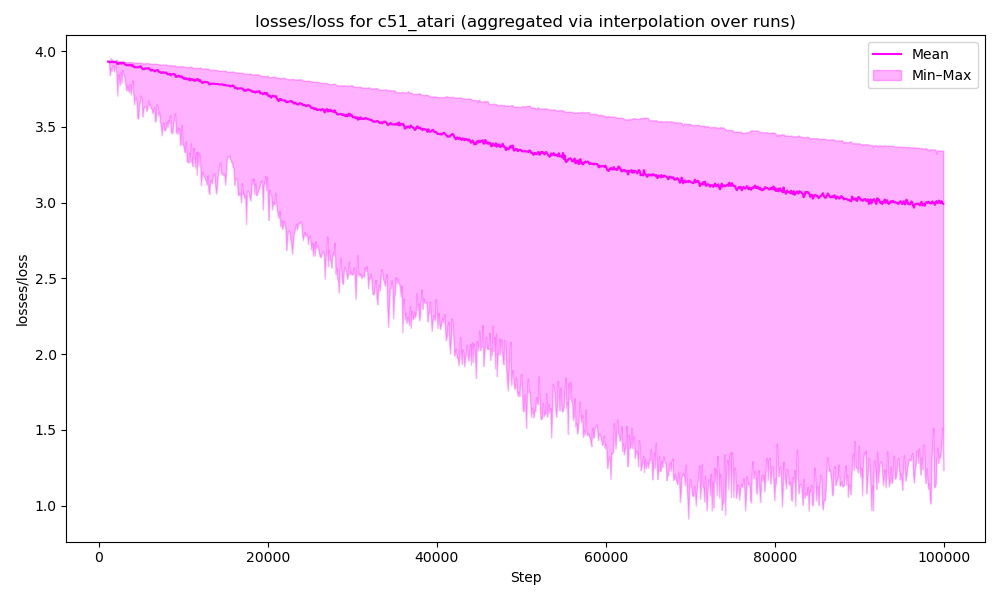
\includegraphics[width=.45\textwidth]{figures/c51/losses_loss_c51_atari.png}
		\label{fig:c51_loss}
	}
	\quad
	\subfloat[][Q-values (\texttt{losses/q\_values}). 
	The mean climbs from near 0 to $\sim 4$--$5$, with outliers reaching 6--7.]{
		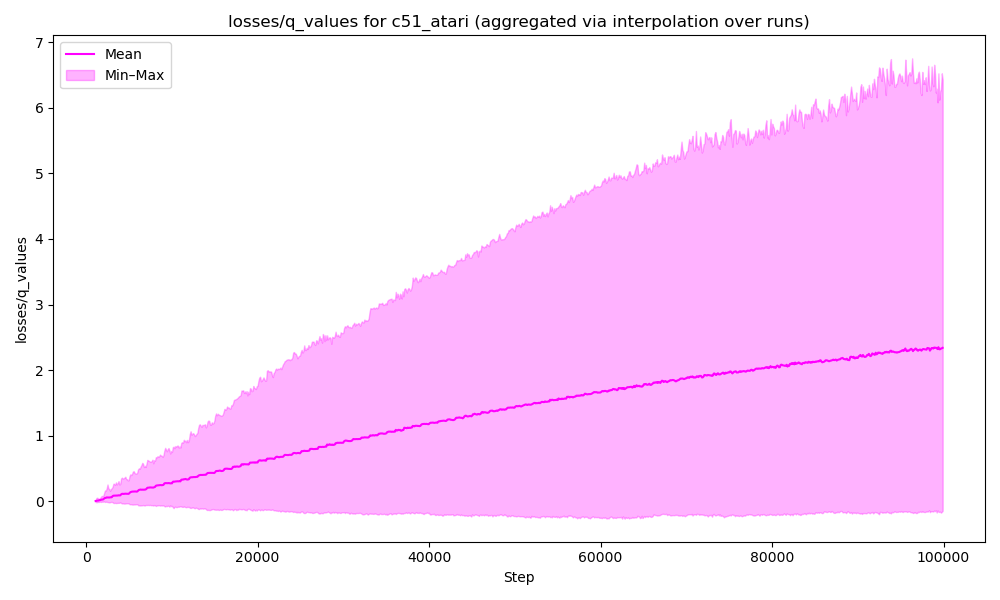
\includegraphics[width=.45\textwidth]{figures/c51/losses_q_values_c51_atari.png}
		\label{fig:c51_q_values}
	}
	\caption{C51 training metrics over 100k steps, aggregated (via interpolation) across 32 runs.}
	\label{fig:c51_training_metrics}
\end{figure}

Figure~\ref{fig:c51_training_metrics} shows that certain runs produce extremely long episodes 
(Figure~\ref{fig:c51_episodic_length}, subfloat~a), 
while the overall \texttt{SPS} curve (subfloat~b) hovers around 140--150 later in training, 
slightly lower than baseline DQN’s $\sim160$. 
The training loss (subfloat~c) descends from near 4.0 to 2.0, 
while distributional \texttt{q\_values} (subfloat~d) broaden significantly.

\paragraph{Episodic Return (Aggregated)}

\begin{figure}
	\centering
	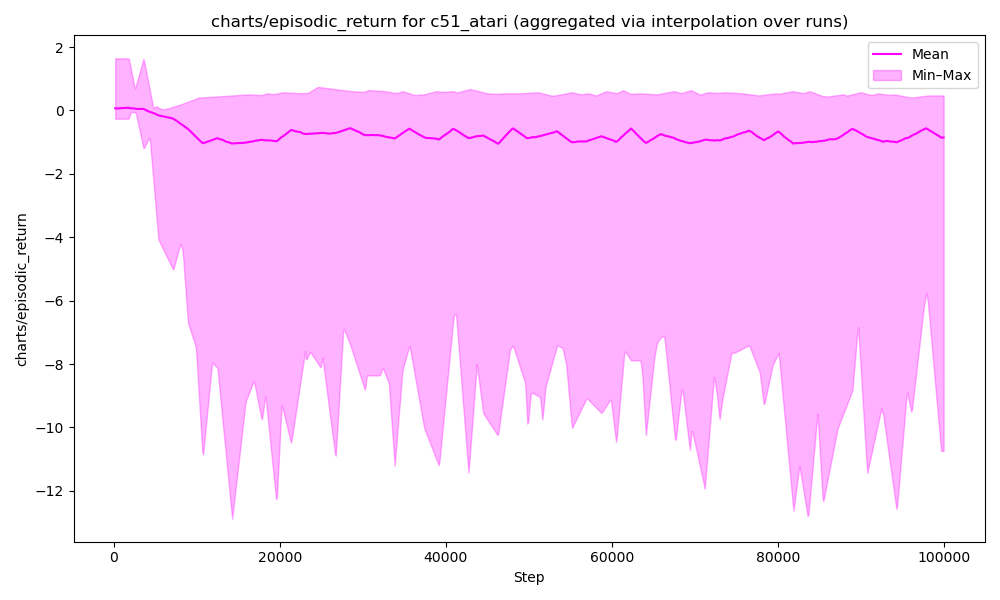
\includegraphics[width=0.6\textwidth]{figures/c51/charts_episodic_return_human_c51_atari.png}
	\caption{C51 episodic return (human-normalized), aggregated over 32 runs. 
		Negative scores dominate, especially due to \emph{Boxing}’s steep dips below -10.}
	\label{fig:c51_return_human}
\end{figure}

\begin{figure}
	\centering
	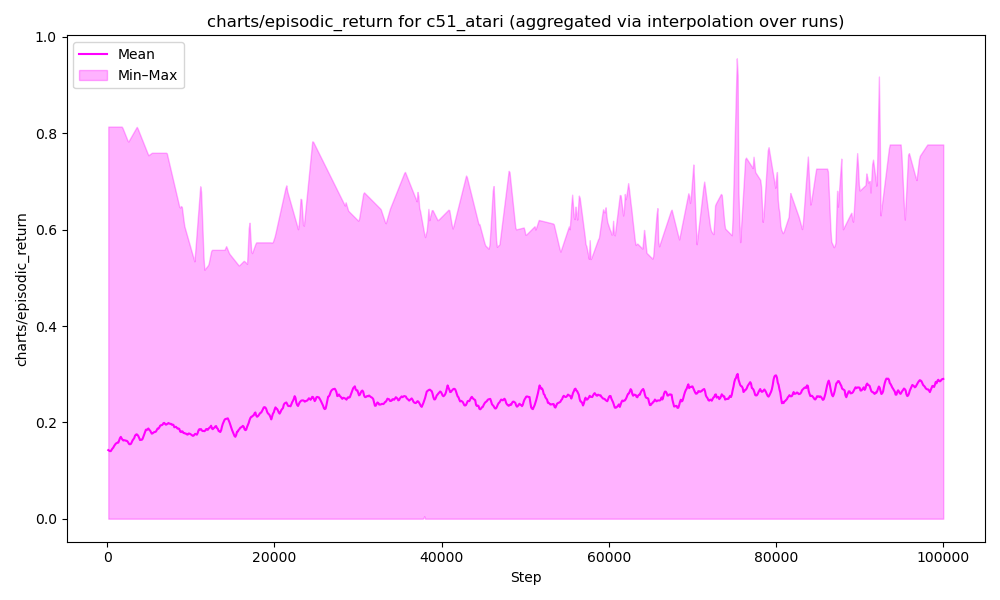
\includegraphics[width=0.6\textwidth]{figures/c51/charts_episodic_return_minmax_c51_atari.png}
	\caption{C51 episodic return (min--max normalized). 
		The mean grows toward 0.25--0.30, indicating moderate performance relative to each game’s min--max range.}
	\label{fig:c51_return_minmax}
\end{figure}

Due to extreme negative performance in certain games, such as \emph{Boxing}, 
the human-normalized return (Figure~\ref{fig:c51_return_human}) 
often falls below -1. In min--max (Figure~\ref{fig:c51_return_minmax}), 
the mean approaches $\sim0.25$--$0.30$ by 100k steps.

\paragraph{Per-Game Returns}

\begin{figure}
	\centering
	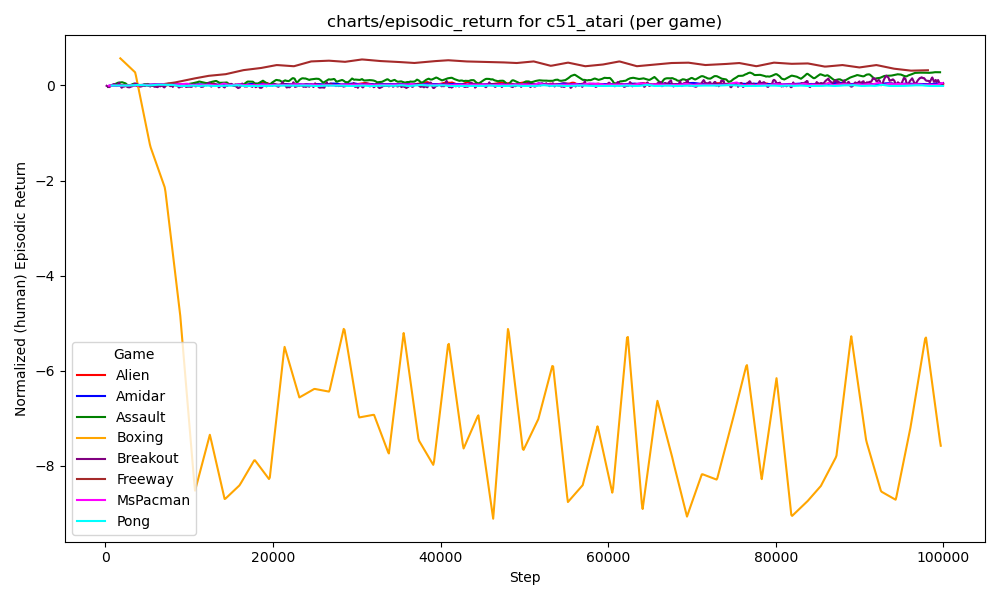
\includegraphics[width=0.6\textwidth]{figures/c51/charts_episodic_return_per_game_human_c51_atari.png}
	\caption{C51 returns per game (human-normalized). 
		\emph{Boxing} (orange) can plunge below -12, dwarfing improvements in other games.}
	\label{fig:c51_return_pergame_human}
\end{figure}

\begin{figure}
	\centering
	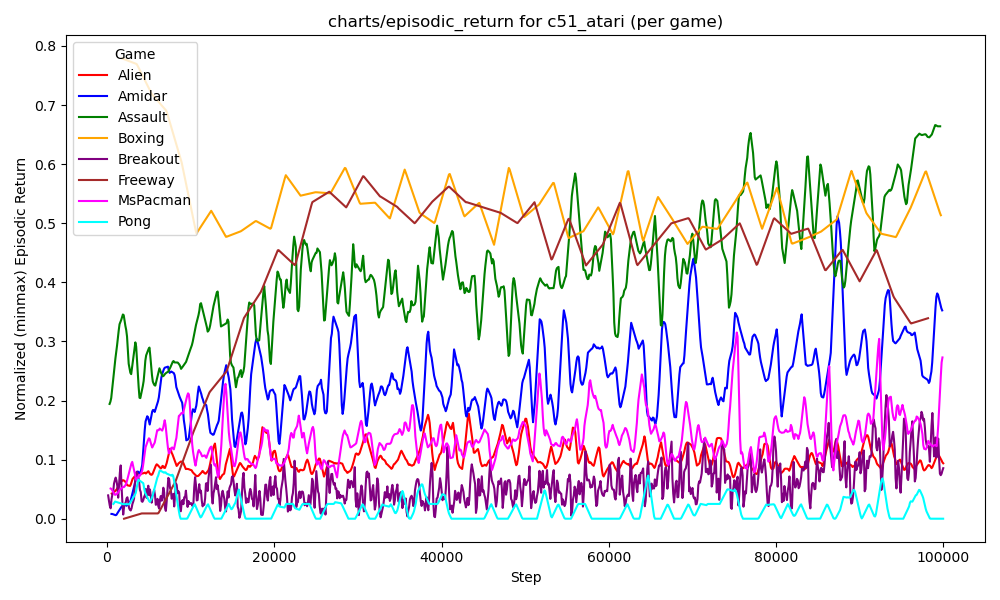
\includegraphics[width=0.6\textwidth]{figures/c51/charts_episodic_return_per_game_minmax_c51_atari.png}
	\caption{C51 returns per game (min--max normalized). 
		\emph{Assault} (green) climbs above 0.5, while \emph{Pong} (cyan) remains near zero.}
	\label{fig:c51_return_pergame_minmax}
\end{figure}

\paragraph{Emissions}

\begin{table}
	\caption{Carbon emissions (kg\,CO\textsubscript{2}eq) for C51 across 32 runs.}
	\label{tab:c51_emissions}
	\centering
	\begin{tabular}{lcccccccc}
		\toprule
		\textbf{Algorithm} & \textbf{mean} & \textbf{std} & \textbf{median} & 
		\textbf{q25} & \textbf{q75} & \textbf{min} & \textbf{max} & \textbf{iqmean} \\
		\midrule
		C51 & 0.007750 & 0.0003042 & 0.007655 & 0.007489 & 0.008099 & 0.007410 & 0.008257 & 0.007679 \\
		\bottomrule
	\end{tabular}
\end{table}

\begin{figure}
	\centering
	\includegraphics[width=0.55\textwidth]{figures/c51/emissions_dqn_c51.png}
	\caption{Mean emissions: C51 (magenta) at $\sim0.00775$\,kg vs.\ DQN (gold) at $\sim0.00647$\,kg.}
	\label{fig:c51_vs_dqn_emissions}
\end{figure}

C51’s mean emissions near 0.00775\,kg exceed DQN’s 0.00647\,kg. 
Distributional overhead (computing 51 probability “atoms”) likely increases GPU usage.

\paragraph{Evaluation Results}

\begin{table}
	\caption{Overall final evaluation (10 episodes each) for C51 across 32 runs.}
	\label{tab:c51_eval_overall}
	\centering
	\begin{tabular}{lcccccccc}
		\toprule
		\textbf{Normalization} & \textbf{mean} & \textbf{std} & \textbf{median} & 
		\textbf{q25} & \textbf{q75} & \textbf{min} & \textbf{max} & \textbf{iqmean} \\
		\midrule
		\textbf{Human}   & -1.0811 & 3.2862 & 0.0 & -0.0132 & 0.0418 & -12.8810 & 0.7770 & 0.00684 \\
		\textbf{Min--Max}& 0.2503 & 0.2568 & 0.2005 & 0.0 & 0.4419 & 0.0 & 0.8270 & 0.13997 \\
		\bottomrule
	\end{tabular}
\end{table}

\begin{table}
	\caption{Per-game final evaluation for C51 (human- vs.\ min--max normalized). 
		Each row aggregates 40 total episodes (10 per seed).}
	\label{tab:c51_eval_gamewise}
	\centering
	\begin{tabular}{llcccc}
		\toprule
		\textbf{Game} & \textbf{Norm} & \textbf{mean} & \textbf{std} & \textbf{min} & \textbf{max}\\
		\midrule
		Alien & Human    & -0.0149 & 0.0127 & -0.0343 & 0.00635 \\
		& Min--Max & 0.0321  & 0.0211 & 0.0     & 0.0675 \\
		\cmidrule{1-6}
		Amidar & Human   & 0.0336  & 0.0153 & 0.00431 & 0.0678 \\
		& Min--Max & 0.2851 & 0.1181 & 0.0599  & 0.5484 \\
		\cmidrule{1-6}
		Assault & Human  & 0.1994  & 0.1467 & -0.0262 & 0.3860 \\
		& Min--Max & 0.5434 & 0.2229 & 0.2005  & 0.8270 \\
		\cmidrule{1-6}
		Boxing & Human   & -9.3869 & 2.6728 & -12.8810 & -4.7857 \\
		& Min--Max & 0.4548  & 0.0870 & 0.3411   & 0.6047 \\
		\cmidrule{1-6}
		Breakout & Human & 0.1478  & 0.2072 & -0.0565 & 0.4751 \\
		& Min--Max & 0.1618 & 0.1641 & 0.0     & 0.4211 \\
		\cmidrule{1-6}
		Freeway & Human  & 0.3632  & 0.3688 & 0.0      & 0.7770 \\
		& Min--Max & 0.3839 & 0.3899 & 0.0     & 0.8214 \\
		\cmidrule{1-6}
		MsPacman & Human & 0.0189  & 0.0176 & -0.0057 & 0.0483 \\
		& Min--Max & 0.1410 & 0.0707 & 0.0419 & 0.2592 \\
		\cmidrule{1-6}
		Pong & Human     & -0.01   & $5.27\times 10^{-18}$ & -0.01 & -0.01 \\
		& Min--Max & 0.0     & 0.0     & 0.0     & 0.0 \\
		\bottomrule
	\end{tabular}
\end{table}

\paragraph{Comparison with Baseline DQN}
Overall, C51’s human-normalized final mean is \textbf{-1.0811}, pulled down by severe negative performance in \emph{Boxing} (around $-9.39$). Even ignoring that outlier, other titles do not significantly outperform baseline DQN’s 0.1353. In min--max scale, C51’s 0.2503 is also lower than DQN’s 0.3802. Emissions, by contrast, are higher ($\sim0.00775\,\mathrm{kg}$ vs.\ DQN’s 0.00647), reflecting the overhead of computing a 51-atom return distribution each update.

\paragraph{Observations}
\begin{itemize}
	\item \textbf{Distributional Advantage:} 
	Although distributional RL can better capture risk or reward variance, 
	100k steps may be insufficient to realize its full potential.
	\item \textbf{Performance:} 
	Human-norm is $-1.0811$ vs.\ DQN’s 0.1353, with many games remaining near/below zero. 
	Min--max is 0.2503 vs.\ 0.3802.
	\item \textbf{Emissions:}
	C51 uses $\sim0.00775\,\mathrm{kg}$ CO\textsubscript{2}-eq, higher than DQN’s 0.00647, 
	likely due to distributional overhead.
	\item \textbf{Target Network Frequency:}
	Testing 1k, 5k, and 10k found 1k gave decent stability and moderate power usage.
\end{itemize}

In summary, C51 did not outperform the baseline DQN in this 100k-step Atari benchmark, 
though distributional RL may yield advantages over longer runs or with additional tuning.


\subsection{Overall Comparison of DQN-Based Algorithms}
\label{subsec:dqn_overall_comparison}

In this section, we synthesize the results of all five DQN-based algorithms:
\begin{itemize}
	\item \textbf{Baseline DQN} (no additional tweaks)
	\item \textbf{Double DQN} (mitigating Q-value overestimation)
	\item \textbf{Prioritized Experience Replay (PER)} (sampling transitions by TD-error priority)
	\item \textbf{Dueling DQN} (separating state-value from advantage)
	\item \textbf{C51} (distributional RL with a categorical return distribution)
\end{itemize}
We compare them on two axes: final performance (evaluated in both human- and min--max-normalized scales) and carbon emissions. 

\paragraph{Aggregated Final Returns and Emissions}
Table~\ref{tab:dqn_overall} compiles the final evaluation means from Sections \ref{subsubsec:dqn_baseline}, \ref{subsubsec:double_dqn}, \ref{subsubsec:per}, \ref{subsubsec:dueling_dqn}, and \ref{subsubsec:c51}. We list each method’s mean episodic return under both normalization schemes, along with its mean carbon footprint. For completeness, we include standard deviations (\texttt{std}) and other statistics where relevant.

\begin{table}[h]
	\caption{Overall final evaluation and emissions for DQN-based algorithms. 
		Human-/min--max-normalized performance are the global means across 32 runs (8 games, 4 seeds). 
		Emissions are reported in kg\,CO\textsubscript{2}-eq. 
		Lower or negative human-norm means indicate below-human performance on average (e.g.\ in \emph{Boxing}), 
		whereas higher min--max means imply better relative scores.}
	\label{tab:dqn_overall}
	\centering
	\begin{tabular}{lccccc}
		\toprule
		& \multicolumn{2}{c}{\textbf{Final Episodic Return (Mean)}} & 
		\multicolumn{1}{c}{\textbf{Emissions}} \\
		\cmidrule(lr){2-3} \cmidrule(lr){4-4}
		\textbf{Algorithm} & \textbf{Human Norm} & \textbf{Min--Max} & \textbf{(kg\,CO\textsubscript{2}-eq)} \\
		\midrule
		\textbf{DQN (baseline)} & 0.1353 & 0.3802 & 0.00647 \\
		\textbf{Double DQN}     & 0.0226 & 0.3737 & 0.00667 \\
		\textbf{PER}            & 0.0607 & 0.3533 & 0.00725 \\
		\textbf{Dueling DQN}    & 0.1860 & 0.3849 & 0.00689 \\
		\textbf{C51}            & $-1.0811$ & 0.2503 & 0.00775 \\
		\bottomrule
	\end{tabular}
\end{table}

\paragraph{Performance Discussion}
\begin{itemize}
	\item \textbf{Dueling DQN} achieves the highest human-norm mean ($0.1860$), 
	though min--max is only slightly above baseline DQN ($0.3849$ vs.\ $0.3802$). 
	Its moderate overhead in computations yields emissions of $0.00689$\,kg, 
	just above baseline.
	\item \textbf{Double DQN} has a low human-norm mean ($0.0226$) but a reasonably strong min--max mean ($0.3737$). 
	Some games suffer from negative outliers (e.g.\ \emph{Boxing}), 
	but overall it matches baseline DQN in relative scale.
	\item \textbf{PER} does not strongly outperform DQN in short (100k-step) training, 
	scoring $0.0607$ human-norm and $0.3533$ min--max, 
	with slightly higher emissions ($0.00725$\,kg). 
	Prioritizing TD errors may show more benefit in longer runs.
	\item \textbf{C51} exhibits the largest negative dip on human-norm ($-1.0811$), 
	largely due to extreme results in \emph{Boxing} and a few other titles, 
	but obtains $0.2503$ in min--max. 
	It also has the largest emissions ($0.00775$\,kg) among these five, 
	reflecting the overhead of a distributional approach with 51 “atoms.”
	\item \textbf{Baseline DQN} remains a strong reference point. 
	Though not best in any single metric, it has decent performance across games (especially $0.3802$ in min--max), 
	while keeping the lowest carbon footprint ($0.00647$\,kg). 
\end{itemize}

%%%%%% tabella con IQM %%%%%%
Table~\ref{tab:dqn_overall_iqm} extends the previous summary
(Table~\ref{tab:dqn_overall})
by including the interquartile mean (IQM)~\cite{agarwal:statistical_precipice}
for each of the three metrics:
\begin{itemize}
	\item \textbf{Human‐Normalized Returns} (mean and IQM)
	\item \textbf{Min--Max Normalized Returns} (mean and IQM)
	\item \textbf{Emissions (kg\,CO\textsubscript{2}-eq)} (mean and IQM)
\end{itemize}
Recall that IQM is a robust estimator of central tendency, 
averaging only the middle 50\% of data points (between the 25th and 75th percentiles),
thus mitigating the impact of extreme outliers.

\begin{table}[htbp]
	\caption{DQN‐Based Algorithms: Final Returns (Human \& Min--Max Norm) \emph{vs.} Emissions,
		including both Mean and Interquartile Mean (IQM). 
		Data are aggregated over 32 runs (8 Atari games $\times$ 4 seeds). 
		Negative human‐norm means can stem from poor performance in certain games 
		(e.g.\ \emph{Boxing} with highly negative scores).}
	\label{tab:dqn_overall_iqm}
	\centering
	\begin{tabular}{lrrrrrr}
		\toprule
		& \multicolumn{2}{c}{\textbf{Human‐Norm Return}} 
		& \multicolumn{2}{c}{\textbf{Min--Max Return}}
		& \multicolumn{2}{c}{\textbf{Emissions (kg\,CO\textsubscript{2})}} \\
		\cmidrule(lr){2-3}\cmidrule(lr){4-5}\cmidrule(lr){6-7}
		\textbf{Algorithm}
		& \textbf{Mean} & \textbf{IQM}
		& \textbf{Mean} & \textbf{IQM}
		& \textbf{Mean} & \textbf{IQM} \\
		\midrule
		\textbf{DQN} 
		& 0.1353 & 0.1137 
		& 0.3802 & 0.3426 
		& 0.00647 & 0.00637 \\
		\textbf{Double DQN} 
		& 0.0226 & 0.0894 
		& 0.3737 & 0.3272 
		& 0.00667 & 0.00656 \\
		\textbf{PER} 
		& 0.0607 & 0.0813 
		& 0.3533 & 0.3087 
		& 0.00725 & 0.00716 \\
		\textbf{Dueling DQN} 
		& 0.1860 & 0.1020 
		& 0.3849 & 0.3454 
		& 0.00689 & 0.00678 \\
		\textbf{C51} 
		& $-1.0811$ & 0.00684 
		& 0.2503 & 0.1400 
		& 0.00775 & 0.00768 \\
		\bottomrule
	\end{tabular}
\end{table}

\paragraph{Discussion.}
\begin{itemize}
	\item \textbf{Human‐Norm vs.\ IQM.} 
	Some methods (\emph{e.g.}, Double DQN, C51) 
	exhibit a large discrepancy between the mean and IQM in human‐normalized returns, 
	indicating a handful of extreme outliers (often due to specific games like \emph{Boxing}).
	\item \textbf{Dueling DQN.} 
	Its mean is highest in human‐norm (0.1860), 
	but the IQM (0.1020) is closer to baseline DQN’s 0.1137, 
	suggesting moderate overall gains once outliers are downweighted.
	\item \textbf{C51’s Negative Mean.} 
	With $-1.08$ in human‐norm, C51 suffers from severely negative outliers; 
	however, its IQM (0.00684) sits just above zero, reflecting that most runs or games 
	are not quite so disastrous outside \emph{Boxing}.
	\item \textbf{Emissions Overhead.} 
	Distributional (C51) and prioritized (PER) methods do have higher carbon costs 
	(around 0.0077\,kg and 0.00725\,kg, respectively) than vanilla DQN (0.00647\,kg). 
	The IQM for emissions shows a similar trend (0.00768 and 0.00716 vs.\ 0.00637).
\end{itemize}

Altogether, adding the IQM metric helps to highlight the presence of large outliers
in short 100k‐step runs. Dueling emerges as a modest improvement on baseline DQN
once extreme seeds are downweighted, whereas C51 and PER do not yet exhibit 
strong benefits for the added cost in short training scenarios.

%%%%%%%%%%%%%%%%%%%%%%%%%%%%%

\paragraph{Scatter Plots of Emissions vs.\ Performance}
To visually depict the trade-off between carbon footprint and final performance,
Figures~\ref{fig:dqn_scatter_mean_iqm} and~\ref{fig:dqn_scatter_mean_mean} 
show scatter plots of \texttt{Mean~Emissions} on the x-axis against 
(\emph{i}) the \texttt{IQMean} or 
(\emph{ii}) the \texttt{Mean} of final evaluation on the y-axis. 
We plot both the human-normalized and min--max normalized variants:

\begin{figure}
	\centering
	\subfloat[][Human Norm: Mean Emissions vs.\ IQMean Evaluation]{
		\includegraphics[width=.45\textwidth]{figures/dqn_based_comparison/scatter_iqmean_human_dqn_based_comparison}
		\label{fig:dqn_scatter_iqm_human}
	}
	\quad
	\subfloat[][Min--Max: Mean Emissions vs.\ IQMean Evaluation]{
		\includegraphics[width=.45\textwidth]{figures/dqn_based_comparison/scatter_iqmean_minmax_dqn_based_comparison.png}
		\label{fig:dqn_scatter_iqm_minmax}
	}
	\caption{Scatter: Mean Emissions vs.\ Interquartile Mean (IQM) final evaluation, for DQN-based algorithms. 
		C51 (magenta) appears far to the right (highest emissions) 
		and near the bottom in human norm, though it’s closer in min--max. 
		DQN and Double DQN cluster with relatively low emissions.}
	\label{fig:dqn_scatter_mean_iqm}
\end{figure}

\begin{figure}
	\centering
	\subfloat[][Human Norm: Mean Emissions vs.\ Mean Evaluation]{
		\includegraphics[width=.45\textwidth]{figures/dqn_based_comparison/scatter_mean_human_dqn_based_comparison.png}
		\label{fig:dqn_scatter_mean_human}
	}
	\quad
	\subfloat[][Min--Max: Mean Emissions vs.\ Mean Evaluation]{
		\includegraphics[width=.45\textwidth]{figures/dqn_based_comparison/scatter_mean_minmax_dqn_based_comparison.png}
		\label{fig:dqn_scatter_mean_minmax}
	}
	\caption{Scatter: Mean Emissions vs.\ Mean final evaluation, for DQN-based algorithms. 
		Again, C51 (magenta) is an outlier with higher emissions and negative (human) or low (min--max) returns. 
		Dueling (blue) has moderate emissions and the highest human-norm performance.}
	\label{fig:dqn_scatter_mean_mean}
\end{figure}

\paragraph{Game-by-Game Observations}
When looking individually per environment:
\begin{itemize}
	\item \textbf{Boxing} heavily skews human-normalized averages for PER and especially C51, 
	yielding strongly negative means. 
	Dueling or Double DQN often handle \emph{Boxing} more stably.
	\item \textbf{Freeway} is comparatively easier, so all variants converge to near-human or above. 
	PER and Dueling both score well here. 
	\item \textbf{Assault} sees moderate or high min--max normalized returns across the board; 
	distributional methods like C51 can do fairly well in some seeds, but not enough to beat DQN or Dueling on average.
\end{itemize}
\begin{figure}[htbp]
	\centering
	\subfloat[][Human Norm: Assault]{
		\includegraphics[width=.45\textwidth]{figures/dqn_based_comparison/charts_episodic_return_human_comparison_AssaultNoFrameskip-v4_dqn.png}
		\label{fig:assault_human}
	}
	\quad
	\subfloat[][Min--Max: Assault]{
		\includegraphics[width=.45\textwidth]{figures/dqn_based_comparison/charts_episodic_return_minmax_comparison_AssaultNoFrameskip-v4_dqn.png}
		\label{fig:assault_minmax}
	}
	\caption{Comparison of DQN-based algorithms on \textbf{Assault}, 
		showing human-normalized (\textbf{left}) and min--max normalized (\textbf{right}) 
		final returns over 100k steps. 
		Distributional methods (e.g.\ C51) can excel in some seeds but not enough to surpass Dueling/DQN on average.}
	\label{fig:assault_comparison}
\end{figure}

%----------------------
% 2) BOXING
%----------------------
\begin{figure}[htbp]
	\centering
	\subfloat[][Human Norm: Boxing]{
		\includegraphics[width=.45\textwidth]{figures/dqn_based_comparison/charts_episodic_return_human_comparison_BoxingNoFrameskip-v4_dqn.png}
		\label{fig:boxing_human}
	}
	\quad
	\subfloat[][Min--Max: Boxing]{
		\includegraphics[width=.45\textwidth]{figures/dqn_based_comparison/charts_episodic_return_minmax_comparison_BoxingNoFrameskip-v4_dqn.png}
		\label{fig:boxing_minmax}
	}
	\caption{Comparison of DQN-based algorithms on \textbf{Boxing}. 
		The human-normalized scale (\textbf{left}) highlights large negative dips, especially for C51 and PER. 
		Min--max normalized (\textbf{right}) shows moderate ranges for most algorithms.}
	\label{fig:boxing_comparison}
\end{figure}

%----------------------
% 3) FREEWAY
%----------------------
\begin{figure}[htbp]
	\centering
	\subfloat[][Human Norm: Freeway]{
		\includegraphics[width=.45\textwidth]{figures/dqn_based_comparison/charts_episodic_return_human_comparison_FreewayNoFrameskip-v4_dqn.png}
		\label{fig:freeway_human}
	}
	\quad
	\subfloat[][Min--Max: Freeway]{
		\includegraphics[width=.45\textwidth]{figures/dqn_based_comparison/charts_episodic_return_minmax_comparison_FreewayNoFrameskip-v4_dqn.png}
		\label{fig:freeway_minmax}
	}
	\caption{Comparison of DQN-based algorithms on \textbf{Freeway}. 
		All methods converge relatively quickly to near-human or above. 
		PER and Dueling typically perform strongly on this environment.}
	\label{fig:freeway_comparison}
\end{figure}


\paragraph{Emissions and Efficiency}
As indicated by both Table~\ref{tab:dqn_overall}, Table~\ref{tab:dqn_overall_iqm}, 
and the scatter plots (Figures~\ref{fig:dqn_scatter_mean_iqm}--\ref{fig:dqn_scatter_mean_mean}), 
\textbf{C51} has the highest mean emissions ($\sim0.00775\,\mathrm{kg}$), 
while \textbf{PER} also exceeds baseline levels at $0.00725\,\mathrm{kg}$. 
\textbf{DQN} remains the lowest ($0.00647\,\mathrm{kg}$). 
In short 100k-step training, the benefits of distributional or prioritized approaches 
do not fully emerge, whereas their computational overhead (and hence emissions) is quite tangible.

\paragraph{Emissions Barplot}

Finally, Figure~\ref{fig:dqn_comp_emissions_bar} illustrates a direct barplot comparison
of the average emissions (with error bars for standard deviation) for the five methods.
\begin{figure}[htb]
	\centering
	\includegraphics[width=0.48\textwidth]{figures/dqn_based_comparison/barplot_emissions_dqn_based_comparison.png}
	\caption{Emissions Barplot (DQN-based Comparison). 
		C51 (magenta) leads with $\sim 0.0078\,\mathrm{kg}$, while DQN (gold) is at the low end ($0.00647$).}
	\label{fig:dqn_comp_emissions_bar}
\end{figure}

\paragraph{Key Takeaways}
\begin{itemize}
	\item \textbf{Dueling DQN} shows the best human-norm mean (0.1860), 
	or second-best min--max (0.3849). Its overhead is modest.
	\item \textbf{Double DQN} is cheap in energy and helps curb Q-value inflation, 
	but does not necessarily raise final returns in short runs (0.0226 human, 0.3737 min--max).
	\item \textbf{PER} is also more costly (0.00725\,kg) with only slight gains in 100k steps, 
	suggesting PER’s advantage might need longer training to appear.
	\item \textbf{C51} is the outlier in both emissions and negative returns (human), 
	though its IQM is far less extreme, indicating that only a few seeds/games are catastrophic.
	\item \textbf{Baseline DQN} remains a viable option at 100k steps, 
	balancing decent performance and the lowest emissions of the five variants.
\end{itemize}


\subsection{Policy-Based Algorithms}
This section presents results for the three policy gradient methods.

\subsubsection{REINFORCE}
\begin{itemize}
	\item Training execution and stability.
	\item Performance scores and energy consumption.
\end{itemize}
Training execution.
Stability of policy gradient training.
Final scores and emissions.


\subsubsection{PPO (Proximal Policy Optimization)}
\begin{itemize}
	\item Effect of clipping on training stability.
	\item Performance vs. REINFORCE.
\end{itemize}
Did clipping help stabilize training?
Efficiency compared to REINFORCE.


\subsubsection{SAC (Soft Actor-Critic)}
\label{subsubsec:sac}
\begin{itemize}
	\item Impact of entropy regularization.
	\item Energy efficiency compared to PPO and REINFORCE.
\end{itemize}
How did the entropy regularization affect performance?
Energy trade-offs (is SAC more expensive to train?).


\subsection{Overall Comparison of Policy-Based Algorithms}
\begin{itemize}
	\item Graphs comparing all policy-based methods.
	\item Which method achieved better stability?
	\item Summary of trade-offs between energy consumption and performance.
\end{itemize}
Graphs comparing policy-based methods.
Which is more stable? Which is more efficient?
Final takeaway: Did one clearly outperform the others in both energy efficiency and reward?


\subsection{Cross-Category Comparison: DQN vs. Policy Gradient}
\begin{itemize}
	\item Which family was more energy-efficient?
	\item Graphs comparing the best-performing models from each category.
	\item Conclusion: Do policy-based methods require more energy but provide better sample efficiency?
\end{itemize}
Which family is generally more energy-efficient?
Graphs comparing best DQN-based vs. best policy-based model.
Final summary of the findings.